%===============================================================================
% LaTeX sjabloon voor de bachelorproef toegepaste informatica aan HOGENT
% Meer info op https://github.com/HoGentTIN/latex-hogent-report
%===============================================================================

\documentclass[dutch,dit,thesis]{hogentreport}

\usepackage{lipsum} % For blind text, can be removed after adding actual content

%% Pictures to include in the text can be put in the graphics/ folder
\graphicspath{{graphics/}}

%% For source code highlighting, requires pygments to be installed
%% Compile with the -shell-escape flag!
%% \usepackage[section]{minted}
%% If you compile with the make_thesis.{bat,sh} script, use the following
%% import instead:
\usepackage[section,outputdir=../output]{minted}
\usemintedstyle{solarized-light}
\definecolor{bg}{RGB}{253,246,227} %% Set the background color of the codeframe

%% Change this line to edit the line numbering style:
\renewcommand{\theFancyVerbLine}{\ttfamily\scriptsize\arabic{FancyVerbLine}}
\setminted[console]{
    bgcolor=bg,
    fontfamily=tt,
    linenos=true,
    numberblanklines=true,
    numbersep=5pt,
    gobble=0,
    framesep=2mm,
    funcnamehighlighting=true,
    tabsize=4,
    obeytabs=false,
    breaklines=true,
    mathescape=false,
    samepage=false,
    showspaces=false,
    showtabs =false,
    texcl=false,
}

\setminted[yaml]{
    bgcolor=bg,
    fontfamily=tt,
    linenos=true,
    numberblanklines=true,
    numbersep=5pt,
    gobble=0,
    framesep=2mm,
    funcnamehighlighting=true,
    tabsize=4,
    obeytabs=false,
    breaklines=true,
    mathescape=false,
    samepage=false,
    showspaces=false,
    showtabs =false,
    texcl=false,
}

\setminted[shell]{
    bgcolor=bg,
    fontfamily=tt,
    linenos=true,
    numberblanklines=true,
    numbersep=5pt,
    gobble=0,
    framesep=2mm,
    funcnamehighlighting=true,
    tabsize=4,
    obeytabs=false,
    breaklines=true,
    mathescape=false,
    samepage=false,
    showspaces=false,
    showtabs =false,
    texcl=false,
}

\setminted[diff]{
    bgcolor=bg,
    fontfamily=tt,
    linenos=true,
    numberblanklines=true,
    numbersep=5pt,
    gobble=0,
    framesep=2mm,
    funcnamehighlighting=true,
    tabsize=4,
    obeytabs=false,
    breaklines=true,
    mathescape=false,
    samepage=false,
    showspaces=false,
    showtabs =false,
    texcl=false,
}

%% Macro definition to load external java source files with \javacode{filename}:
\newmintedfile[javacode]{java}{
    bgcolor=bg,
    fontfamily=tt,
    linenos=true,
    numberblanklines=true,
    numbersep=5pt,
    gobble=0,
    framesep=2mm,
    funcnamehighlighting=true,
    tabsize=4,
    obeytabs=false,
    breaklines=true,
    mathescape=false
    samepage=false,
    showspaces=false,
    showtabs =false,
    texcl=false,
}

% Other packages not already included can be imported here
\usepackage{parskip}
\usepackage{caption}
\newenvironment{longlisting}{\captionsetup{type=listing}}{}
\def\code#1{\texttt{#1}}

%%---------- Document metadata -------------------------------------------------
\author{Anton Van Assche}
\supervisor{Dhr. T. Clauwaert}
\cosupervisor{Dhr. B. Deferme}
\title%
    {De identiteit van een Linux-systeem:\\ Onderzoek en Proof-of-Concept.}
\academicyear{\advance\year by -1 \the\year--\advance\year by 1 \the\year}
\examperiod{1}
\degreesought{\IfLanguageName{dutch}{Professionele bachelor in de toegepaste informatica}{Bachelor of applied computer science}}
\partialthesis{false} %% To display 'in partial fulfilment'
%\institution{Internshipcompany BVBA.}

%% Add global exceptions to the hyphenation here
\hyphenation{back-slash}

%% The bibliography (style and settings are  found in hogentthesis.cls)
\addbibresource{bachproef.bib}            %% Bibliography file
\addbibresource{../voorstel/voorstel.bib} %% Bibliography research proposal
\defbibheading{bibempty}{}

%% Prevent empty pages for right-handed chapter starts in twoside mode
\renewcommand{\cleardoublepage}{\clearpage}

\renewcommand{\arraystretch}{1.2}

%% Content starts here.
\begin{document}

%---------- Front matter -------------------------------------------------------

\frontmatter

\hypersetup{pageanchor=false} %% Disable page numbering references
%% Render a Dutch outer title page if the main language is English
\IfLanguageName{english}{%
    %% If necessary, information can be changed here
    \degreesought{Professionele Bachelor toegepaste informatica}%
    \begin{otherlanguage}{dutch}%
       \maketitle%
    \end{otherlanguage}%
}{}

%% Generates title page content
\maketitle
\hypersetup{pageanchor=true}

%%=============================================================================
%% Voorwoord
%%=============================================================================

\chapter*{\IfLanguageName{dutch}{Woord vooraf}{Preface}}%
\label{ch:voorwoord}

%% TODO:
%% Het voorwoord is het enige deel van de bachelorproef waar je vanuit je
%% eigen standpunt (``ik-vorm'') mag schrijven. Je kan hier bv. motiveren
%% waarom jij het onderwerp wil bespreken.
%% Vergeet ook niet te bedanken wie je geholpen/gesteund/... heeft

\lipsum[1-2]
%%=============================================================================
%% Samenvatting
%%=============================================================================

% TODO: De "abstract" of samenvatting is een kernachtige (~ 1 blz. voor een
% thesis) synthese van het document.
%
% Een goede abstract biedt een kernachtig antwoord op volgende vragen:
%
% 1. Waarover gaat de bachelorproef?
% 2. Waarom heb je er over geschreven?
% 3. Hoe heb je het onderzoek uitgevoerd?
% 4. Wat waren de resultaten? Wat blijkt uit je onderzoek?
% 5. Wat betekenen je resultaten? Wat is de relevantie voor het werkveld?
%
% Daarom bestaat een abstract uit volgende componenten:
%
% - inleiding + kaderen thema
% - probleemstelling
% - (centrale) onderzoeksvraag
% - onderzoeksdoelstelling
% - methodologie
% - resultaten (beperk tot de belangrijkste, relevant voor de onderzoeksvraag)
% - conclusies, aanbevelingen, beperkingen
%
% LET OP! Een samenvatting is GEEN voorwoord!

%%---------- Nederlandse samenvatting -----------------------------------------
%
% TODO: Als je je bachelorproef in het Engels schrijft, moet je eerst een
% Nederlandse samenvatting invoegen. Haal daarvoor onderstaande code uit
% commentaar.
% Wie zijn bachelorproef in het Nederlands schrijft, kan dit negeren, de inhoud
% wordt niet in het document ingevoegd.

\IfLanguageName{english}{%
\selectlanguage{dutch}
\chapter*{Samenvatting}
\lipsum[1-4]
\selectlanguage{english}
}{}

%%---------- Samenvatting -----------------------------------------------------
% De samenvatting in de hoofdtaal van het document

\chapter*{\IfLanguageName{dutch}{Samenvatting}{Abstract}}

Het onderwerp van cyberbeveiliging en de automatisering van systemen zijn beide van groot belang in de IT-wereld.
Toch is het samenvoegen van deze twee onderwerpen niet altijd vanzelfsprekend voor elk bedrijf.
Met de nieuwe NIS2-richtlijn, oftewel "Network and Information Security", worden bedrijven verplicht om hun systemen te beschermen tegen cyberaanvallen.
De reikwijdte van sectoren die onder deze richtlijn vallen, is aanzienlijk uitgebreid ten opzichte van zijn voorganger.
Een van de verplichtingen die bedrijven moeten nakomen, is het in kaart brengen van alle kritieke systemen die van invloed zijn op hun bedrijfsvoering.

Infrastructure as Code kan een oplossing bieden voor dit vraagstuk.
Door de huidige infrastructuur van een bedrijf te beschrijven in code, biedt het een overzicht van alle gebruikte systemen.
Toch vinden veel bedrijven, met name KMO's, het moeilijk om over te stappen naar een Infrastructure as Code omgeving.
Dit kan verschillende redenen hebben, zoals een gebrek aan kennis, tijd en budget.

Deze bachelorproef richt zich op het onderzoeken van mogelijke tools die kunnen helpen bij de overstap naar een Infrastructure as Code omgeving door het opstellen van een configuratie-inventaris.
Er zal worden gekeken naar bestaande tools die hieraan kunnen bijdragen.
Daarnaast zal er een analyse worden gemaakt van de verschillende eigenschappen van Linux-systemen die het beste kunnen worden opgenomen in een configuratie-inventaris.

Vervolgens zal er een Proof of Concept worden ontwikkeld, waarin een Bash-script zal worden geschreven dat basisinformatie van een Linux-systeem verzamelt en omzet in een verzameling van overzichtelijke bestanden.
Dit script zal worden uitgevoerd op vijf verschillende Debian servers, elk met hun eigen rol binnen de omgeving.

Deze bachelorproef verkent het gebruik van tools zoals Nmap en LinPEAS-ng voor het ontdekken van de configuratie van een Linux-systeem.
Nmap wordt voornamelijk ingezet voor het verkennen van netwerkconfiguraties, terwijl LinPEAS-ng dieper inzicht biedt in de configuratie van het Linux-systeem zelf en potentiële beveiligingsrisico's identificeert.
Het ontwikkelde script vormt een solide basis waarop beheerders kunnen voortbouwen door extra functionaliteiten toe te voegen en oplossingen te vinden voor eventuele beperkingen die tijdens de ontwikkeling van het script zijn geïdentificeerd.


%---------- Inhoud, lijst figuren, ... -----------------------------------------

\tableofcontents

% In a list of figures, the complete caption will be included. To prevent this,
% ALWAYS add a short description in the caption!
%
%  \caption[short description]{elaborate description}
%
% If you do, only the short description will be used in the list of figures

\listoffigures

% If you included tables and/or source code listings, uncomment the appropriate
% lines.
\listoftables
\listoflistings

% Als je een lijst van afkortingen of termen wil toevoegen, dan hoort die
% hier thuis. Gebruik bijvoorbeeld de ``glossaries'' package.
% https://www.overleaf.com/learn/latex/Glossaries

%---------- Kern ---------------------------------------------------------------

\mainmatter{}

% De eerste hoofdstukken van een bachelorproef zijn meestal een inleiding op
% het onderwerp, literatuurstudie en verantwoording methodologie.
% Aarzel niet om een meer beschrijvende titel aan deze hoofdstukken te geven of
% om bijvoorbeeld de inleiding en/of stand van zaken over meerdere hoofdstukken
% te verspreiden!

%%=============================================================================
%% Inleiding
%%=============================================================================

\chapter{\IfLanguageName{dutch}{Inleiding}{Introduction}}%
\label{ch:inleiding}

\section{\IfLanguageName{dutch}{Probleemstelling}{Problem Statement}}%
\label{sec:probleemstelling}

In het begin van 2023, op 6 januari, werd de NIS-richtlijn, wat staat voor "Network and Information Security", opgevolgd door zijn nieuwe versie, NIS2.
Deze update bracht verschillende nieuwe voorschriften met zich mee op het gebied van cyberbeveiliging, en het aantal sectoren dat aan deze richtlijnen moet voldoen, werd aanzienlijk uitgebreid.
Enkele sectoren die onder de NIS2 richtlijnen vallen zijn, maar niet beperkt tot~\autocite{NIS2Directive2022}:
\begin{itemize}
    \item Energie: elektriciteit, olie, gas, stadsverwarming en waterstof
    \item Transport: lucht, spoor, water en weg
    \item Digital infrastructuur: Telecom, DNS, TLD, datacenters, vertrouwensdiensten, clouddiensten, \ldots
    \item Digitale diensten: zoekmachines, online markten, sociale netwerken, \ldots
\end{itemize}

Het valt op dat de meeste sectoren die onder de NIS2-richtlijnen vallen, niet per se gericht zijn op IT.
Echter zijn bedrijven tegenwoordig in toenemende mate afhankelijk van bepaalde IT-processen die een impact hebben op hun bedrijfsvoering.
Dit maakt het noodzakelijk om ook cyberbeveiligingswetgevingen op hen toe te passen.

De lidstaten van de Europese Unie hebben tot oktober 2024~\autocite{NIS2Directive2022} de tijd om deze nieuwe richtlijnen in hun nationale wetgeving te implementeren.
Dit geeft bedrijven een beperkte periode om hun processen aan te passen aan deze nieuwe wetgeving, een uitdaging die vooral voor kleine of middelgrote ondernemingen (KMO's) problematisch kan zijn, gezien hun vaak beperkte middelen.

Een van de essenti\"ele vereisten van deze richtlijnen is dat bedrijven verplicht zijn om een ``inventory of assets'' op te stellen voor alle systemen en operaties die ze gebruiken.
Deze bachelorproef richt zich specifiek op het bieden van een oplossing voor KMO's, binnen sectoren die nu wel moeten voldoen aan deze richtlijnen, voor het inventariseren van Linux-systemen hun configuratie, waarbij de focus ligt op het vergemakkelijken van het naleven van deze nieuwe regelgeving.

Een manier die op dit moment veel gebruikt wordt om een inventaris van systemen en de configuratie ervan is het gebruik maken van Infrastructure as Code, ook wel IaC genoemd.
Het is een concept dat de laatste jaren steeds meer aan populariteit wint. Voornamelijk doordat het beheerders van computernetwerken in staat stelt om hun configuratie en infrastructuur vast te leggen in code, in plaats van handmatig te configureren.
Binnen deze code kunnen veelvoorkomende, complexe taken automatisch worden uitgevoerd, en dit alles op een geteste en foutloze manier~\autocite{chef-what-is-iac}.
Hier zullen we later verder op ingaan in hoofstuk~\ref{ch:stand-van-zaken}.

\section{\IfLanguageName{dutch}{Onderzoeksvraag}{Research question}}%
\label{sec:onderzoeksvraag}

\begin{enumerate}
    \item Hoe kunnen bedrijven, met name KMO's, zich aanpassen aan de nieuwe vereisten van de NIS2-richtlijn, met name met betrekking tot het opstellen van een ``inventory of assets'' voor hun IT-systemen?
    \item Op welke manieren kan Infrastructure as Code (IaC) worden ingezet om het inventariseren van systemen en configuraties te vergemakkelijken en te voldoen aan de eisen van de NIS2-richtlijn?
    \item Welke tools en technieken kunnen worden gebruikt om de configuratie en infrastructuur van Linux-systemen vast te leggen en te beheren?
    \item Welke configuratie-eigenschappen van Linux-systemen zijn essentieel om in kaart te brengen voor een inventaris?
\end{enumerate}

\section{\IfLanguageName{dutch}{Onderzoeksdoelstelling}{Research objective}}%
\label{sec:onderzoeksdoelstelling}

Het doel van deze bachelorproef is om een Proof of Concept te ontwikkelen die KMO's helpt bij het inventariseren van hun Linux-systemen en hun configuratie, met behulp van een Bash-script.
Het script zal rekening moeten houden met de bevindingen uit de risicoanalyse, en voorgaande hoofdstukken van deze bachelorproef.

Ook zal er een kritische evaluatie worden gemaakt van de Proof of Concept, waarbij de effectiviteit en volledigheid van de inventarisatie wordt beoordeeld.

\section{\IfLanguageName{dutch}{Opzet van deze bachelorproef}{Structure of this bachelor thesis}}%
\label{sec:opzet-bachelorproef}

% Het is gebruikelijk aan het einde van de inleiding een overzicht te
% geven van de opbouw van de rest van de tekst. Deze sectie bevat al een aanzet
% die je kan aanvullen/aanpassen in functie van je eigen tekst.

De rest van deze bachelorproef is als volgt opgebouwd:

In Hoofdstuk~\ref{ch:stand-van-zaken} wordt een overzicht gegeven van de stand van zaken binnen het onderzoeksdomein, op basis van een literatuurstudie.

In Hoofdstuk~\ref{ch:methodologie} wordt de methodologie toegelicht en worden de gebruikte onderzoekstechnieken besproken om een antwoord te kunnen formuleren op de onderzoeksvragen.

In Hoofdstuk~\ref{ch:linux-server-concepten} richten we ons op enkele fundamentele concepten van Linux-servers.

In Hoofdstuk~\ref{ch:computernetwerk-concepten} behandelen we de essenti\"ele concepten van computernetwerken in relatie tot servers.

In Hoofdstuk~\ref{ch:risicoanalyse} wordt een risicoanalyse uitgevoerd op de configuratie van Linux-servers, op basis van voorgaande hoofdstukken.

In Hoofdstuk~\ref{ch:poc} wordt een proof-of-concept uitgewerkt, waarbij de bevindingen van de risicoanalyse worden toegepast in een Bash-script.

In Hoofdstuk~\ref{ch:conclusie}, tenslotte, wordt de conclusie gegeven en een antwoord geformuleerd op de onderzoeksvragen. Daarbij wordt ook een aanzet gegeven voor toekomstig onderzoek binnen dit domein.

\chapter{\IfLanguageName{dutch}{Stand van zaken}{State of the art}}%
\label{ch:stand-van-zaken}

% Tip: Begin elk hoofdstuk met een paragraaf inleiding die beschrijft hoe
% dit hoofdstuk past binnen het geheel van de bachelorproef. Geef in het
% bijzonder aan wat de link is met het vorige en volgende hoofdstuk.

% Pas na deze inleidende paragraaf komt de eerste sectiehoofding.

\section{Network and Information Security 2}%
\label{sec:nis2}

\section{Huidige aanpak van asset management}%
\label{sec:huidige_aanpak_van_asset_management}

\subsection{Infrastructure as Code}%
\label{sub:iac}

Sinds de opkomst van computernetwerken is het uitrollen en beheren van servers en netwerken altijd een uitdagende taak geweest.
Infrastructure as Code (IaC) is een concept dat de laatste jaren steeds meer aan populariteit wint. Dit komt vooral doordat het beheerders van zulke netwerken in staat stelt om hun configuratie en infrastructuur vast te leggen in code, in plaats van handmatig te configureren.
Binnen deze code kunnen veelvoorkomende, complexe taken automatisch worden uitgevoerd, en dit alles op een geteste en foutloze manier~\autocite{chef-what-is-iac}.

IaC is gebaseerd op drie fundamentele concepten~\autocite{chef-what-is-iac}:
\begin{itemize}
    \item Automatisering: Het aanpassen van handmatige configuratie en het uitrollen van nieuwe servers worden allemaal geautomatiseerd met behulp van code.
    \item Testen: IT en DevSecOps processen kunnen met vertrouwen worden uitgevoerd omdat de code getest is.
    \item Idempotentie: Processen worden niet alleen toegepast op nieuwe servers, maar ook op bestaande servers om een consistente configuratie te behouden.
\end{itemize}

E\'en van de grootste voordelen van Iac is de verhoging van de effici\"entie~\autocite{splunk-benefits-iac}.
Doordat veel taken geautomatiseerd worden, kunnen beheerders zich richten op andere, meer complexe taken.
Zo heeft Red Hat in 2016 een casestudy gepubliceerd~\autocite{case-study-nasa-iac} waarin ze NASA's resultaten van hun overstap naar de IaC-tools Ansible en Ansible Tower hebben geanalyseerd.
Hierin geven ze aan dat het updateproces van nasa.gov van meer dan 1 uur is teruggebracht tot minder dan 5 minuten.
Het langdurige proces van het patchen van updates werd teruggebracht van een proces dat meerdere dagen in beslag nam naar een proces van ongeveer 45 minuten.

Het Duitse Federaal Ministerie van Voedsel en Landbouw (Bundesanstalt f\"ur Landwirtschaft und Ern\"ahrung, of BLE), heeft ook bepaalde IT-toepassingen met 50\% kunnen versnellen dankzij een overstap naar een IaC-aanpak~\autocite{case-study-ble-iac}.
In de studie bespreken ze kort waarom ze hebben besloten over te schakelen naar een IaC-aanpak en geven ze een paar voorbeelden van hoe ze voorheen te werk gingen en hoe ze dit met IaC hebben aangepakt.
Tijdens de implementatie hebben ze 1000 virtuele machines overgeschakeld van Debian en SUSE Linux naar Red Hat Enterprise Linux, ook bekend als RHEL.
Deze machines worden beheerd met behulp van Satellite en geautomatiseerd met Ansible.

Condition assessments is één van de belangrijkste componenten van IT asset management (IAM)~\autocite{ibm-what-is-iam}.
Dit proces houdt in dat men op elk moment de huidige staat kan bekijken van een asset.
Doordat IaC de configuratie van een asset vastlegt in code en zorgt dat deze consistent is, kan IaC ondersteuning bieden bij dit proces.

\subsection{Data Center Infrastructure Management}
\label{sub:dcim}

\subsection{IP Address Management}
\label{sub:ipam}

\subsection{Snipe-IT}
\label{sub:snipe-it}

Snip-IT is een open-source webapplicatie ontwikkeld door Grokability sinds 2013~\autocite{snipe-it-introduction}, die gericht is op IT-assetmanagement.
Het idee achter Snipe-IT komt voort uit de vroegere aanpak van het bedrijf, toen het voornamelijk nog gebruik maakte van spreadsheets om hun bedrijfsmiddelen te inventariseren.
Het doel was om een applicatie te ontwikkelen die deze taak op een meer georganiseerde en effici\"ente manier kon uitvoeren.

\begin{figure}[h!]
    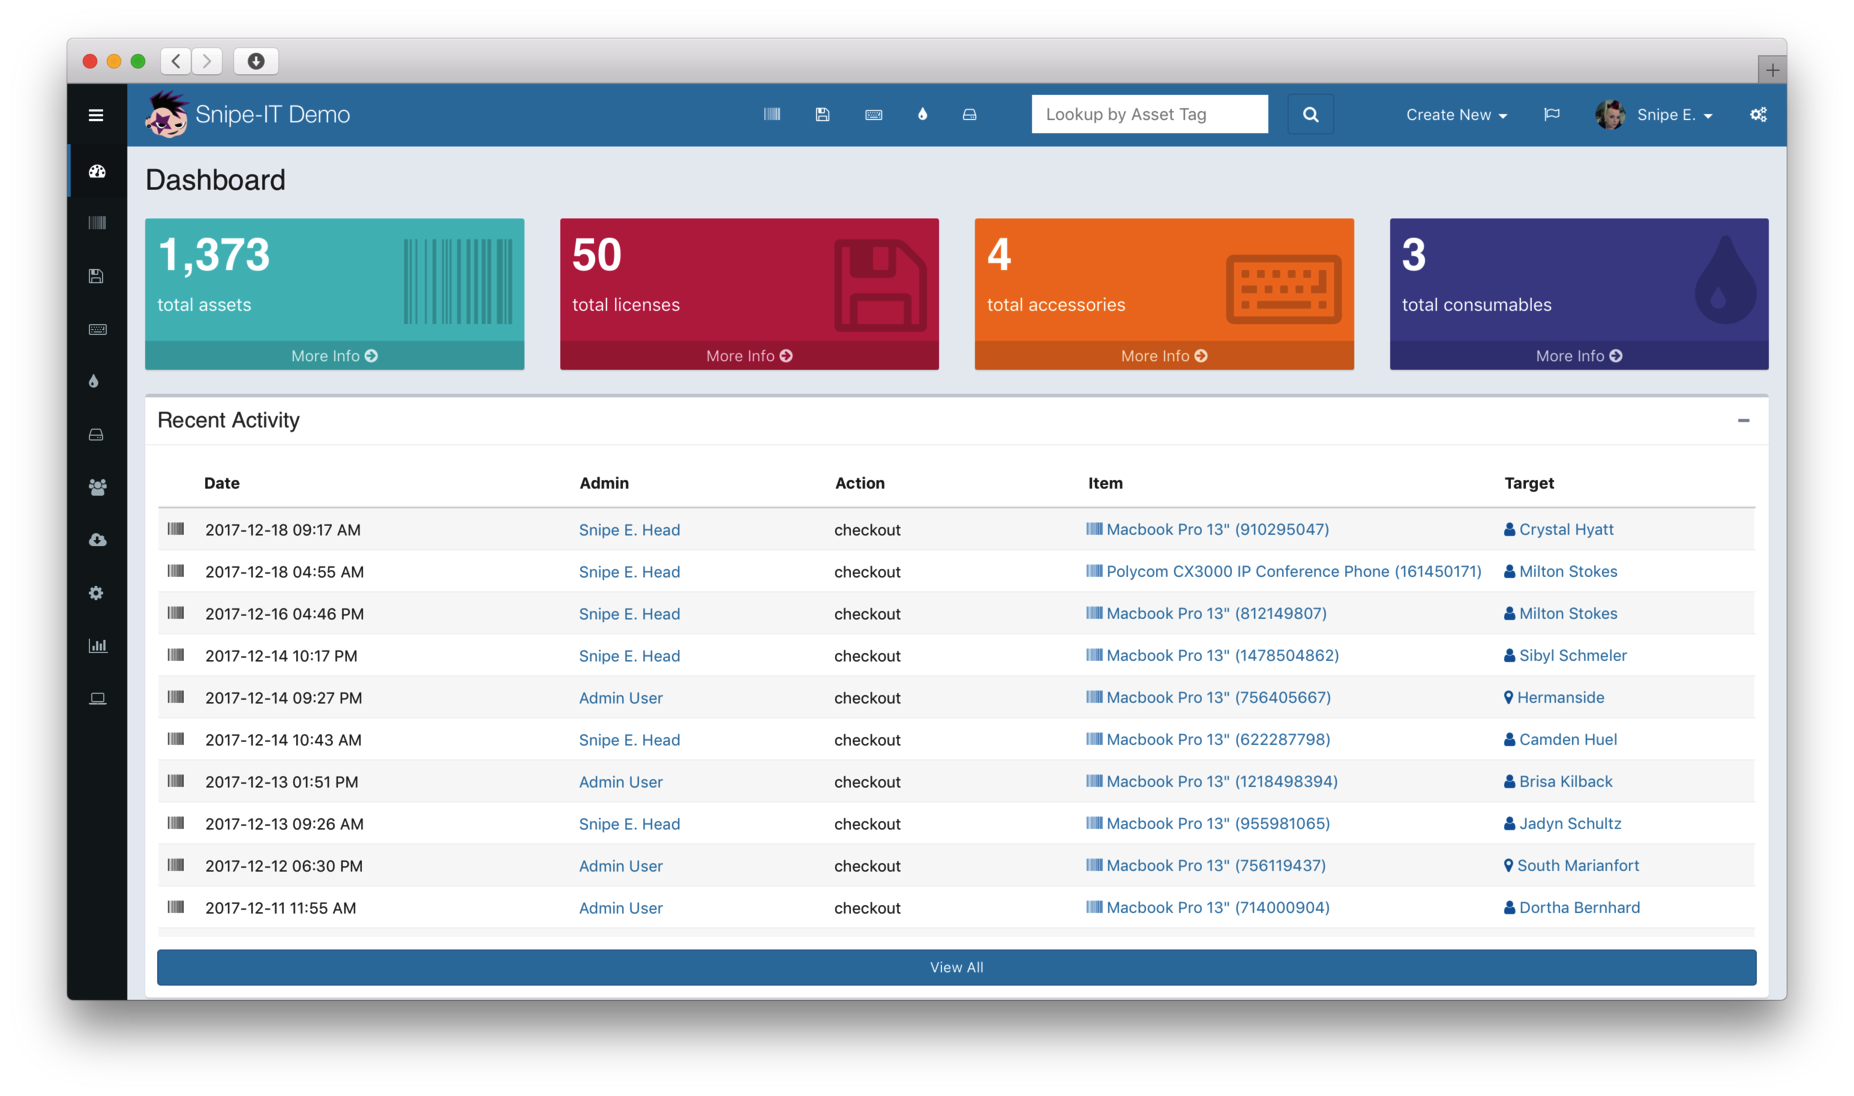
\includegraphics[width=\textwidth]
    {./graphics/snipe-dashboard.png}
    \caption{\label{fig:snipe-it-dashboard}Snip-IT dashboard waarin we het totale aantal assets binnen de organisatie kunnen zien, alsook een oplijsting van verschillende toestellen recent toegekend zijn~\autocite{snipe-it-dashboard}.}
\end{figure}

De software biedt een gebruiksvriendelijke webinterface (\ref{fig:snipe-it-dashboard}) waarmee bedrijfsmiddelen, licenties, garanties en meer gemakkelijk kunnen worden beheerd.
Wanneer men kiest voor de self-hosted optie is de software gratis beschikbaar, terwijl ook verschillende cloud-gebaseerde optie beschikbaar zijn tegen een jaarlijkse bijdrage.
Deze prijs varieert afhankelijk van de nodige features en support.
Alle code en services gerelateerd aan Snipe-IT zijn vrij beschikbaar op GitHub~\autocite{snipe-it-github}.

Enkele van de belangrijkste functies van Snipe-IT zijn~\autocite{snipe-it-features}, maar zijn niet beperkt tot:
\begin{itemize}
    \item Gemakkelijk zien welke assets zijn toegewezen, aan wie, en hun fysieke locatie
    \item In één klik inchecken
    \item Assetmodellen waarmee je gemeenschappelijke functies kunt groeperen
    \item Vereisen van Gebruikersacceptatie (Eindgebruikers EULA's/Gebruiksvoorwaar-\ den) bij Uitchecken
    \item E-mailmeldingen voor het verlopen van garanties en licenties
    \item Integratie met de meeste handheld barcode scanners en QR-codelezer apps
    \item Snelle en eenvoudige asset-audit
    \item Voeg je eigen aangepaste velden toe voor extra assetattributen
    \item Assets gemakkelijk importeren en exporteren
    \item Genereer QR-code labels voor eenvoudige mobiele toegang en labeling
    \item Assets gemarkeerd als aanvraagbaar kunnen worden aangevraagd door een gebruiker
    \item Assets behouden een volledige geschiedenis inclusief uitchecken, inchecken en onderhoud
    \item Optionele digitale handtekeningen bij assetacceptatie
\end{itemize}

\subsection{Nagios}
\label{sub:nagios}

\subsection{Lansweeper}
\label{sub:lansweeper}

Lansweeper, opgericht in 2004, is een Belgisch commercieel IT discovery \& inventory platform~\autocite{lansweeper-history}.
Het is een veelgebruikte tool voor het scannen, bijhouden en beheren van IT-assets binnen een organisatie.
Met functionaliteiten voor zowel hardware- als software-inventarisatie, biedt Lansweeper gebruikers een uitgebreid overzicht van alle IT-assets in hun netwerk.

Het grote voordeel van Lansweeper ten opzichte van andere tools, zoals Snipe-IT, is dat het een volledig geautomatiseerde oplossing biedt~\autocite{lansweeper-features}.
Dit betekent dat het platform in staat is om automatisch alle IT-assets binnen een netwerk te detecteren, zonder handmatige configuratie of de noodzaak om op elk systeem een agent te installeren~\autocite{lansweeper-getting-started}.
Een scan zal essenti\"ele informatie verzamelen over het asset, zoals de versie van het besturingssysteem, de hostname van de machine, het MAC-adres en de laatst ingelogde gebruiker.
Dit gebeurt met behulp van verschillende protocollen, waaronder SNMP.
De gedetecteerde informatie wordt vervolgens opgeslagen in een centrale database en is toegankelijk via een gebruiksvriendelijke webinterface.

\begin{figure}[h!]
    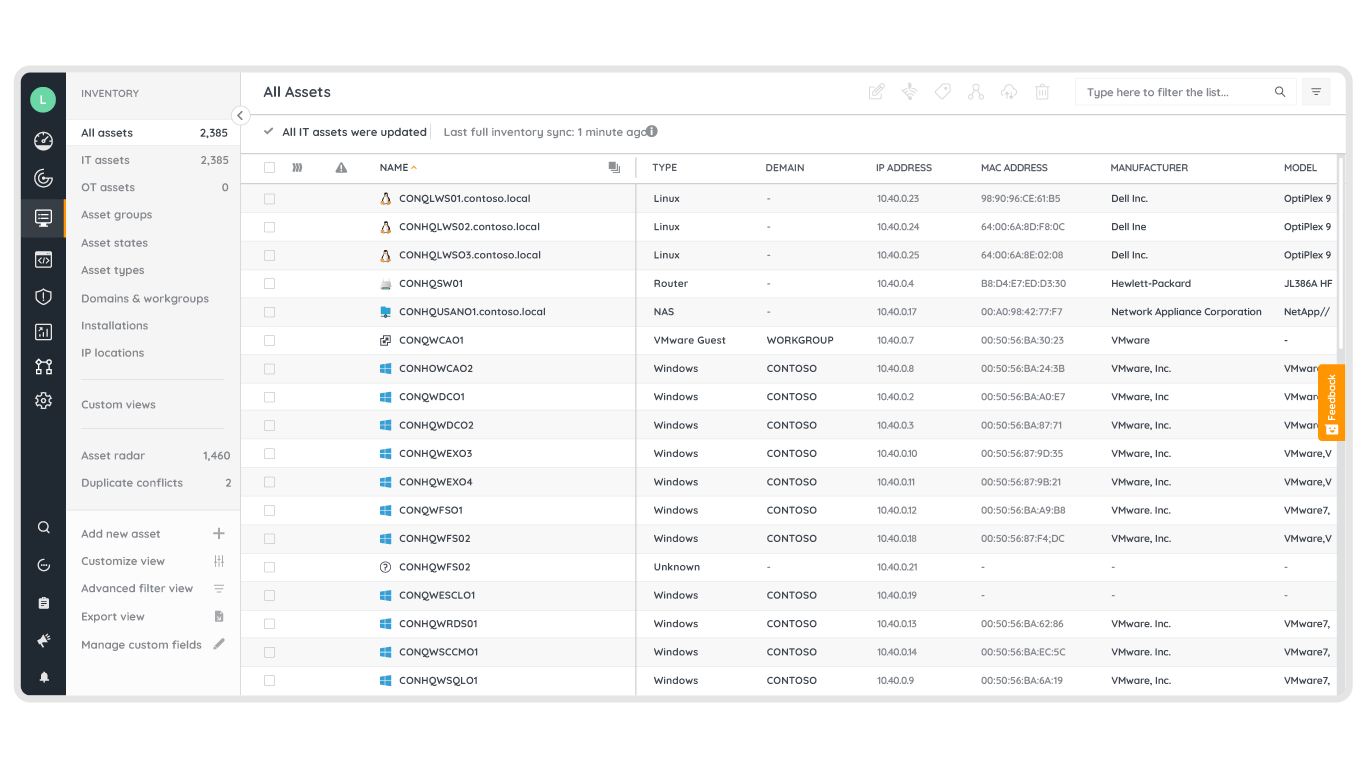
\includegraphics[width=\textwidth]
    {./graphics/lansweeper-dashboard.png}
    \caption{\label{fig:lansweeper-dashboard}Lansweeper dashboard.}
\end{figure}

Gebruikers kunnen aangepaste rapporten genereren over verschillende aspecten van hun IT-infrastructuur, zoals hardwareconfiguraties, softwarelicenties, patchniveaus en meer~\autocite{lansweeper-features}.
Deze rapporten zijn bruikbaar voor audits, nalevingscontroles en capaciteitsplanning.

Naast het genereren van rapporten en het identificeren van nieuwe IT-assets, biedt Lansweeper ook de mogelijkheid om rogue devices op het netwerk te detecteren.
Deze detectie gebeurt door continu het netwerk te scannen en alle gevonden assets te vergelijken met de resultaten in de database van bekende assets.
Wanneer een apparaat wordt gedetecteerd dat niet voorkomt in de database, genereert Lansweeper een waarschuwing, waardoor beheerders en administrators actie kunnen ondernemen.
Bovendien heeft Lansweeper de capaciteit om mogelijke beveiligingsrisico's te identificeren binnen uw inventaris door gebruik te maken van de NIST National Vulnerability Database~\autocite{lansweeper-cam}.

%%=============================================================================
%% Methodologie
%%=============================================================================

\chapter{\IfLanguageName{dutch}{Methodologie}{Methodology}}%
\label{ch:methodologie}

\section{Stand van zaken}
\label{sec:stand-van-zaken}
Dit onderdeel belicht de actuele benadering van configuration management, met een specifieke focus op Infrastructure as Code (IaC).
Naast een definitie van IaC worden de essenti\"ele componenten ervan besproken, evenals de voordelen die het met zich meebrengt.
Bovendien worden tools genoemd die kunnen worden ingezet om de configuratie van een systeem te identificeren en later om te zetten naar een IaC-omgeving.

Daarnaast zal er ook aandacht worden besteed aan asset management en hoe dit kan helpen bij de overgang van een niet-IaC-omgeving naar een IaC-omgeving.
Hoewel asset management minder gericht is op de configuratie van individuele machines, biedt het wel inzicht in de infrastructuur en de assets die beheerd moeten worden.
Op basis van deze informatie kunnen vervolgens de initi\"ele configuraties worden vastgelegd in code,

\section{Linux Server Concepten}
\label{sec:linux-server-concepten}
Dit hoofdstuk richt zich op de fundamentele concepten van Linux-servers.
Het doel is om een dieper begrip te bieden van de verschillende componenten en functies van een Linux-systeem, evenals de relevante ondersteunende tools.
Door deze basisbegrippen te verkennen, kunnen we effectiever bepalen welke informatie moet worden opgenomen in onze configuratie-inventaris.

\section{Computernetwerk Concepten}
\label{sec:computernetwerk-concepten}
Dit hoofdstuk behandelt de essenti\"ele concepten van computernetwerken in relatie tot servers.
We zullen verkennen hoe netwerkconnectiviteit een integraal onderdeel is van de functionaliteit van servers en hoe verschillende concepten en technologie\"en worden toegepast om deze connectiviteit te realiseren.

\section{Het opstellen van een configuratie-inventaris}
\label{sec:risicoanalyse}
In dit hoofdstuk zullen we een risicoanalyse uitvoeren voor Linux-systemen.
We zullen de bevindingen uit de eerdere hoofdstukken combineren om een lijst van cruciale configuratie-eigenschappen te presenteren voor het beheer en de beveiliging van Linux-systemen.
Door gebruik te maken van literatuuronderzoek en de besproken concepten, zullen we de risico's identificeren waaraan Linux-systemen blootstaan en welke specifieke eigenschappen moeten worden opgenomen in onze configuratie-inventaris.

\section{Proof of Concept}
\label{sec:proof-of-concept}
Dit hoofdstuk omvat de praktische toepassing van onze bevindingen.
We zullen een Bash-script ontwikkelen en uitvoeren op 5 virtuele Debian-servers, elk met hun eigen unieke taken en eigenschappen.
Dit stelt ons in staat om de bruikbaarheid en effectiviteit van onze aanpak te testen in een real-world scenario.

We zullen ook de gevonden resultaten analyseren en beoordelen of de configuratie-inventaris voldoet aan de verwachtingen en of deze als basis kan dienen voor een Infrastructure as Code (IaC)-omgeving.
Dit wordt gedaan door de resultaten te vergelijken met de bevindingen uit de risicoanalyse en de configuratie-inventaris.

%%=============================================================================
%% Linux server concepten
%%=============================================================================

\chapter{\IfLanguageName{dutch}{Linux server concepten}{Linux server concepts}}%
\label{ch:linux-server-concepten}

\section{Inleiding}
\label{linux_inleiding}

Om ons te helpen bij het maken van een configuratie-inventaris van een Linux systeem, moeten we verschillende aspecten van Linux in acht nemen.
Door enkele basisconcepten te kennen over de verschillende componenten en functies van een Linux systeem en de beschikbare ondersteunende tools, is het veel eenvoudiger om te bepalen wat we in onze inventaris moeten opnemen en wat niet.
In dit hoofdstuk worden enkele basisbegrippen van Linux uitgelegd, zoals wat het is en wat er deel van uitmaakt, enz.

\section{Het Linux besturingssysteem}
\label{linux_linux_besturingssysteem}

Een besturingsysteem is de software die applicaties toe laat om te communiceren met de hardware van een computer.
Vaak als we spreken over besturingssystemen, denken we aan Windows, macOS of Linux.
Echter is Linux hier een buitenbeentje, aangezien het niet een besturingssysteem is, maar een kernel.
De taak van de kernel is om de hardware van een computer te beheren en de software die op de computer draait te ondersteunen.

De kernel is het hart van een Linux-systeem, en is verantwoordelijk voor het beheer van de hardware van de computer, zoals de CPU, het geheugen, de opslag en de netwerkinterfaces.
Echter wanneer we spreken over een Linux-systeem, bedoelen we vaak de bundel van software die samen met de kernel wordt geleverd, zoals de GNU core-utils, de shell en de grafische interface.
Deze bundeling van software gaan we vaak een Linux-distributie noemen, of ook wel een distro genoemd.
Enkele bekende Linux-distributies zijn Debian, Ubuntu, Fedora en RHEL.

Een typisch Linux-systeem bestaat uit verschillende lagen, zoals te zien is in figuur~\ref{fig:linux-system-structure}.
De user space is diegene waar de gebruiker het meeste mee in contact komt, hier draaien de applicaties en de shell.
Applicaties hebben beperkte rechten, zo kunnen ze zelf geen hardware aanspreken, of aansturen.
Dit moet gebeuren door de Application Programming Interface (API) die de kernel aanbiedt, die system calls doet naar de kernel space, wat te zien is in figuur~\ref{fig:linux-system-structure}~\autocite{mauerer2008linux}.

\begin{figure}[h!]
    \begin{center}
        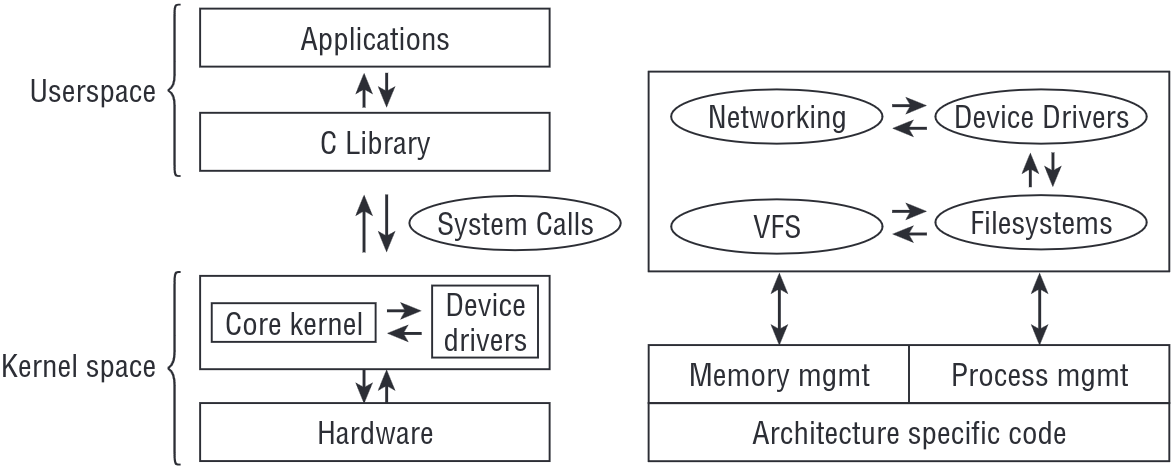
\includegraphics[width=\textwidth]
        {./graphics/linux/kernel-structure.png}
        \caption[Structuur van Linux-systeem.]{\label{fig:linux-system-structure}Structuur van een typisch Linux-systeem~\autocite{mauerer2008linux}}
    \end{center}
\end{figure}

De Linux-kernel is wat we noemen een monolithische kernel, wat wil zeggen dat het een enkele grote binary is die alle functionaliteit bevat.
Dit houdt in dat alle subsystemen van de kernel, zoals het bestandssysteem, het geheugenbeheer en de netwerkstack, in dezelfde binary zitten.
Echter is de kernel wel modulair, wat wil zeggen dat we modules kunnen laden en lossen in de kernel, zonder dat we de kernel zelf moeten hercompileren.
Deze modules kunnen voor verschillende doeleinden worden gebruikt, zoals het toevoegen van ondersteuning voor nieuwe hardware, het beveiligen van het systeem met SELinux of AppArmor, of het toevoegen van nieuwe functionaliteit aan de kernel~\autocite{hypponen2021securing}.
Een voorbeeld van een module is \texttt{vboxdrv}, die nodig is om VirtualBox te kunnen gebruiken op een Linux-systeem.

\subsection{Applicatie beheer}
\label{linux_applicatie_beheer}

\subsubsection{Packaging systemen}
\label{linux_packaging_systemen}

Er bestaan vandaag de dag duizenden Linux-distributies die elk hun eigen manier van applicatiebeheer hebben.
Deze diversiteit komt tot uiting in de manier waarop ze hun pakketten beheren.
Toch kunnen de meeste van deze systemen grofweg worden ingedeeld in twee hoofdcategorie\"en: RHEL-gebaseerde systemen en Debi-\ an-gebaseerde systemen.

RHEL-gebaseerde systemen maken gebruik van het Red Hat Package Manager (RPM) systeem, terwijl Debian-gebaseerde systemen vertrouwen op het Debian Package Manager (DPKG) systeem.
Deze twee packaging-systemen vormen de ruggengraat van het applicatiebeheer op hun respectievelijke distributies.
Een beknopt overzicht van de distributies die deze packaging-systemen gebruiken, wordt gepresenteerd in tabel~\ref{table:packaging-systems}.

\begin{table}[!h]
    \begin{center}
        \begin{tabular}{ c c  }
            \hline
                Packaging systeem & Distributies\\ [0.5ex] 
            \hline
            Debian Package Manager (DPKG)     & Debian, Ubuntu, Linux Mint \\
            Red Hat Package Manager (RPM)     & RHEL, Fedora, openSUSE \\
        \end{tabular}
    \end{center}
    \caption[Overzicht van packaging systemen.]{Overzicht van de verschillende packaging systemen en de distributies die ze gebruiken~\autocite{shotts2019linux}.}
    \label{table:packaging-systems}
\end{table}

Hoewel RHEL- en Debian-gebaseerde distributies de dominante spelers zijn, zijn er enkele uitzonderingen op deze regel.
Sommige distributies hebben hun eigen unieke package manager, zoals Arch Linux met pacman, of Gentoo met Portage.
Niettemin behoren de meeste andere distributies tot de RHEL- of Debian-families, en maken ze gebruik van RPM of DPKG voor hun applicatiebeheer.

\subsubsection{Package managers}
\label{linux_package_managers}

De package manager speelt een essenti\"ele rol bij het beheer van software op een systeem.
Het stelt gebruikers in staat om software te installeren, te verwijderen en bij te werken, en zorgt ervoor dat eventuele afhankelijkheden van software adequaat worden beheerd.
Bovendien is versiebeheer een belangrijk aspect van package managers, waarbij de juiste versie van de software wordt ge\"installeerd en up-to-date wordt gehouden door de package manager.

We kunnen de package manager ook inzetten om een lijst van ge\"installeerde softwarepakketten te bekijken, iets wat we later in dit werk zullen gebruiken om een configuratie-inventaris te maken.
Op Debian-gebaseerde systemen kunnen we dit bijvoorbeeld doen door het commando \texttt{apt list -{}-installed} als de root-gebruiker uit te voeren.
Als alternatief kan men ook \texttt{dpkg-query -l} gebruiken, wat ons toelaat om query's uit te voeren op de DPKG-database, zoals te zien in listing~\ref{lst:dpkg-query}.

\begin{listing}
  \begin{minted}[linenos,tabsize=4,breaklines]{console}
vagrant@srv1:~$ sudo dpkg-query -Wf '"${Package}" "${Version}" "${Source}"\n'
"adduser" "3.134" ""
"apparmor" "3.0.8-3" ""
"apt" "2.6.1" ""
"apt-listchanges" "3.24" ""
"apt-utils" "2.6.1" "apt"
"base-files" "12.4+deb12u5" ""
"base-passwd" "3.6.1" ""
"bash" "5.2.15-2+b2" "bash (5.2.15-2)"
"bash-completion" "1:2.11-6" ""
"bind9-dnsutils" "1:9.18.24-1" "bind9"
[...]
  \end{minted}
    \caption[Lijst van ge\"{i}nstalleerde softwarepakketten.]{Uitvoer van het \texttt{dpkg-query} commando om een lijst van ge\"installeerde softwarepakketten te tonen.}
  \label{lst:dpkg-query}
\end{listing}

\subsubsection{Repositories}
\label{linux_repositories}

De meeste package managers halen hun softwarepakketten uit zogenaamde repositories, die dienen als centrale opslagplaatsen voor gebruikers om softwarepakketten te downloaden en te installeren.
Deze repositories bevatten vaak duizenden softwarepakketten die allemaal beheerd kunnen worden door de package manager~\autocite{shotts2019linux}.

Dergelijke repositories worden doorgaans beheerd door de distributie zelf, maar het komt ook vaak voor dat ge\"interesseerde gebruikers bijdragen aan het onderhouden van de pakketten in de repository.
Bovendien bieden de meeste package managers de flexibiliteit om extra repositories toe te voegen, waardoor gebruikers software kunnen installeren die niet beschikbaar is in de standaard repositories.

Een voorbeeld hiervan is Ubuntu, dat gebruikers de mogelijkheid biedt om PPAs toe te voegen, wat staat voor Personal Package Archives.
Deze PPAs worden onderhouden door individuele gebruikers en bevatten software die niet in de standaard repositories van Ubuntu te vinden is.
Een vergelijkbare functionaliteit wordt aangeboden door Fedora met COPR, wat staat voor Cool Other Package Repositories.

\subsection{Bestandssystemen}
\label{linux_bestandssystemen}

Het bestandssysteem is een belangrijk onderdeel van een Linux-systeem, en is verantwoordelijk voor het makkelijk toegang verlenen tot opslagmedia, zoals Hard Drive Disks (HDD's), Solid State Drive (SSD's) en USB-sticks.
Naast het toegang verlenen tot opslagmedia, is het bestandssysteem ook verantwoordelijk voor het beheren van bestanden en directories, en het toekennen van permissies aan deze bestanden en directories.
Dit gebeurt door middel van twee verschillende delen, de collectie van bestanden en directories, en de metadata die hieraan is gekoppeld.
Deze metadata bevat informatie zoals de eigenaar van het bestand, de groep waartoe het bestand behoort, de permissies die zijn toegekend aan het bestand en de timestamps van de creatie, wijziging en toegang van het bestand.
De verzamelnaam voor deze metadata worden ook wel de bestandsattributen genoemd~\autocite{silberschatz2013os}
Verschillende bestandssystemen kunnen worden gebruikt op een Linux-systeem, zoals ext4, xfs, btrfs en zfs.

\begin{listing}
  \begin{minted}[linenos,tabsize=4,breaklines]{console}
[root@fedorable ~]# tree -L 1 /
/
├── afs
├── bin -> usr/bin
├── boot
├── dev
├── etc
├── home
├── lib -> usr/lib
├── lib64 -> usr/lib64
├── lost+found
├── media
├── mnt
├── opt
├── proc
├── root
├── run
├── sbin -> usr/sbin
├── srv
├── sys
├── tmp
├── usr
└── var
  \end{minted}
    \caption[Hi\"{e}rarchische structuur van Linux-bestandssysteem.]{Uitvoer van het \texttt{tree}-commando op een Fedora Linux-systeem om de hi\"erarchische structuur van het Linux-bestandssysteem te tonen.}
  \label{lst:linux-root-dir-structure}
\end{listing}

Linux maakt gebruik van een hi\"erarchisch bestandssysteem, wat wil zeggen dat bestanden en directories worden georganiseerd in een boomstructuur, zoals te zien is in listing~\ref{lst:linux-root-dir-structure}.
Startend vanuit de root directory, die wordt aangeduid met een schuine streep (\texttt{/}), worden bestanden en directories georganiseerd in verschillende niveaus van subdirectories.
Elke directory binnen de root directory kan op zijn beurt bestanden en subdirectories bevatten, met elk hun eigen doel en functie.
Zo heeft de \texttt{etc} directory, staande voor ``et cetera'', de configuratiebestanden voor verschillende softwarepakketten, terwijl de \texttt{bin} directory de binaries bevat die nodig zijn om het systeem te laten functioneren~\autocite{linuxfoundation-filesystem}.

\subsection{Gebruikers en groepen}
\label{linux_gebruikers_groepen}

De Linux-kernel biedt ondersteuning voor het gelijktijdig beheren van meerdere gebruikers, waarbij elke gebruiker wordt onderscheiden aan de hand van hun User ID (UID).
Een gebruiker vertegenwoordigt een entiteit die toegang heeft tot het systeem en de mogelijkheid heeft om bestanden en directories te maken en te bewerken.
Het concept van gebruikers is essentieel om de toegangsrechten en permissies op het systeem te beheren, waardoor een gecontroleerde en veilige omgeving wordt gecre\"eerd.
In veel gevallen heeft elk proces in de user-space zijn eigen gebruiker, die de rechten en permissies van dat proces bepaalt~\autocite{ward2021linux}.

Linux-systemen bevatten typisch meerdere gebruikersaccounts, met als eerste de superuser, die wordt ge\"identificeerd door een UID van 0, zoals weer te geven in listing~\ref{lst:linux-root-id}, en alle rechten heeft op het systeem.
Daarnaast kunnen gebruikersaccounts worden onderverdeeld in twee categorie\"en: systeemgebruikers en normale gebruikers.
Systeemgebruikers hebben doorgaans een UID lager dan 1000 en worden vaak gebruikt voor het draaien van services, zoals een Apache-webserver of een MySQL-database.
Aan de andere kant worden normale gebruikers ge\"identificeerd door een UID hoger dan 1000 en worden ze gebruikt door individuen die het systeem actief gebruiken, zoals systeembeheerders. Een voorbeeld van de uitvoer van het \texttt{id} commando voor een normale gebruiker is te zien in listing~\ref{lst:linux-anton-id}.

\begin{listing}
  \begin{minted}[linenos,tabsize=4,breaklines]{console}
[root@fedorable ~]# id
uid=0(root) gid=0(root) groups=0(root)
  \end{minted}
    \caption[UID, GID en groepslidmaatschap voor superuser.]{Uitvoer van het \texttt{id}-commando voor de superuser, waarop we kunnen zien dat de gebruiker een UID van 0 heeft, een GID van 0 heeft en lid is van de groep \texttt{root}.}
  \label{lst:linux-root-id}
\end{listing}

\begin{listing}
  \begin{minted}[linenos,tabsize=4,breaklines]{console}
[anton@fedorable ~]$ id
uid=1000(anton) gid=1000(anton) groups=1000(anton),10(wheel)
  \end{minted}
    \caption[UID, GID en groepslidmaatschap voor normale gebruiker.]{Uitvoer van het \texttt{id}-commando voor een normale gebruiker, waarop we kunnen zien dat de gebruiker een UID van 1000 heeft, een GID van 1000 heeft en lid is van de groepen \texttt{anton} en \texttt{wheel}.}
  \label{lst:linux-anton-id}
\end{listing}

Naast individuele gebruikers kunnen gebruikers ook worden gegroepeerd in groepen, die een verzameling van gebruikers vertegenwoordigen met dezelfde rechten en permissies.
Groepen worden ook ge\"identificeerd door een unieke Group ID (GID), waarmee ze kunnen worden ge\"identificeerd en beheerd binnen het systeem.
Het gebruik van gebruikers en groepen biedt een gestructureerde manier om de toegangscontrole en beveiliging op een Linux-systeem te beheren, waardoor een geordende en veilige werkomgeving wordt bevorderd.
Zo hebben gebruikers die tot de wheel groep behoren op RHEL-gebaseerde systemen, zoals Fedora en AlmaLinux, de mogelijkheid om root-privileges te verkrijgen door het uitvoeren van het \texttt{sudo} commando.

\begin{table}[!h]
    \begin{adjustbox}{width=1\textwidth}
        \begin{tabular}{ c c  }
            \hline
                Afkorting & Betekenis\\ [0.5ex] 
            \hline
                Gebruikers & Een entiteit die toegang heeft tot het systeem en bestanden en directories kan maken en bewerken. \\
                Groepen    & Een verzameling van gebruikers die dezelfde rechten en permissies hebben. \\
                UID        & Staande voor User ID, is een uniek nummer dat aan een gebruiker wordt toegekend. \\
                GID        & Staande voor Group ID, is een uniek nummer dat aan een groep wordt toegekend. \\
        \end{tabular}
    \end{adjustbox}
    \caption[Terminologie voor gebruikers en groepen.]{Overzicht van terminologie voor gebruikers en groepen.}
    \label{table:user-group-terminology}
\end{table}

Het \texttt{sudo} commando zal natuurlijk enkel werken als de gebruiker die het commando uitvoert, is toegevoegd aan de correcte groep in de \texttt{/etc/sudoers} file.
Als alternatief kan men ook een bestand dat bepaalde regels bevat aanmaken in de \texttt{/etc/sudoers.d/} directory, zoals te zien in listing~\ref{lst:linux-sudoers}.
Dit bestand bevat de verschillende regels die bepalen welke gebruikers en groepen root-privileges kunnen verkrijgen door het uitvoeren van het \texttt{sudo} commando, alsook wat ze kunnen uitvoeren.
Zo kan men bijvoorbeeld specifi\"eren dat een bepaalde gebruiker geen wachtwoord moet ingeven bij het uitvoeren van het \texttt{sudo} commando in combinatie met een bepaald commando.
Een voorbeeld van een \texttt{sudo}-regel is te zien in listing~\ref{lst:linux-sudoers}.

\begin{listing}
  \begin{minted}[linenos,tabsize=4,breaklines]{console}
[root@fedorable ~]# cat /etc/sudoers.d/anton
anton    ALL=(ALL)    NOPASSWD: /usr/bin/dnf
  \end{minted}
    \caption[Inhoud van \texttt{/etc/sudoers.d/anton}.]{Uitvoer van het \texttt{cat}-commando dat de inhoud van het bestand \texttt{/etc/sudoers.d/anton} laat zien. Hieruit blijkt dat de gebruiker \texttt{anton} root-privileges heeft voor het uitvoeren van het \texttt{dnf}-commando en geen wachtwoord hoeft in te voeren bij dit commando.}
  \label{lst:linux-sudoers}
\end{listing}

\subsection{Taakbeheer}
\label{linux_taakbeheer}

Services en processen vormen de ruggengraat van een Linux-systeem, waarbij ze cruciale taken uitvoeren en resources beheren om de algehele functionaliteit te ondersteunen.
Het correct beheren van deze services en processen is van vitaal belang voor de stabiliteit, prestaties en beveiliging van het systeem.

In dit gedeelte zullen we dieper ingaan op twee belangrijke aspecten van het beheer van services en processen op een Linux-systeem: systemd en cronjobs.

\subsubsection{Systemd}
\label{linux_systemd}

Systemd fungeert als een init-systeem op vele Linux-systemen, waardoor het mogelijk is om services te starten, stoppen en beheren als een user-space daemon tijdens het opstartproces.
In vergelijking met zijn voorgangers, zoals SysVinit en Upstart, biedt systemd aanzienlijk meer functionaliteit en wordt het vaak ingezet als een uitgebreide systeem- en servicebeheerder~\autocite{ward2021linux}.

Een van de krachtige kenmerken van systemd is het gebruik van unit files, die de configuratie van verschillende eenheden, zoals services, timers, sockets, devices en mount points, bevatten.
Hierdoor kunnen beheerders niet alleen services beheren, maar ook andere types eenheden.
Een overzicht van enkele veelgebruikte unit types wordt weergegeven in tabel~\ref{table:sytemd_unit_types}.

\begin{table}[!h]
    \begin{center}
        \begin{tabular}{ c c }
            \hline
                Unit type & Omschrijving \\ [0.5ex] 
            \hline
                Service & Een service die op de achtergrond draait en een bepaalde taak uitvoert. \\
                Timer   & Een timer die periodiek een service activeert. \\
                Device  & Een apparaat dat door het systeem wordt beheerd. \\
                Mount   & Een mount point voor een bestandssysteem. \\
        \end{tabular}
    \end{center}
    \caption[Veelvoorkomende unit types in systemd.]{Overzicht van veelvoorkomende unit types in systemd.}
    \label{table:sytemd_unit_types}
\end{table}

Bovendien biedt systemd een mechanisme om afhankelijkheden tussen services te definiëren, waardoor het mogelijk is om complexe opstartvolgordes en -vereisten te beheren.
Met opties zoals \texttt{requires}, \texttt{wants}, \texttt{before} en \texttt{after} kunnen beheerders nauwkeurig aangeven welke services afhankelijk zijn van elkaar en in welke volgorde ze moeten worden gestart.
Dit draagt bij aan de fouttolerantie en consistentie van het systeem~\autocite{ward2021linux}.

Beheerders hebben de mogelijkheid om aangepaste unit files te maken en te bewerken in de \texttt{/etc/systemd/system/} of \texttt{/usr/lib/systemd/system/} directories, waardoor ze volledige controle hebben over de configuratie van services en andere eenheden~\autocite{ward2021linux}.

\subsubsection{Cronjobs}
\label{linux_cronjobs}

Cronjobs zijn geautomatiseerde taken die periodiek worden uitgevoerd op een Linux-systeem, zoals het maken van back-ups, het uitvoeren van systeemupdates of het genereren van rapporten.
Het zorgt ervoor dat we onafhankelijk van het progamma, op een bepaald tijdstip of interval, een bepaalde taak kunnen uitvoeren.
Dit gebruikmakende van de \texttt{cron} daemon, die de cronjobs beheert en uitvoert op de achtergrond.

Men kan cronjobs defini\"eren door middel van cron-tabellen, die de configuratie van de cronjobs bevatten.
Deze tabellen worden opgeslagen in de \texttt{/etc/cron.d/} directory, en kunnen worden bewerkt met behulp van de \texttt{crontab} commando~\autocite{ward2021linux}.

Een typische cron-tabel bestaat uit vijf velden, die de minuut, het uur, de dag van de maand, de maand en de dag van de week aangeven waarop de taak moet worden uitgevoerd.
Na de tijdvelden volgt het commando dat moet worden uitgevoerd, zoals te zien is in figuur~\ref{fig:cronjob-structure}, waar de structuur van een cron-tabel wordt weergegeven~\autocite{ward2021linux}.

\begin{figure}[h!]
    \begin{center}
        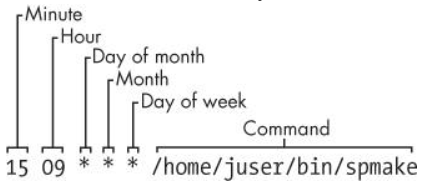
\includegraphics[width=200pt]
        {./graphics/linux/cronjob-structure.png}
        \caption[Structuur van een cron-tabel.]{\label{fig:cronjob-structure}Structuur van een cron-tabel~\autocite{ward2021linux}.}
    \end{center}
\end{figure}

\section{Linux server beveiliging}
\label{linux_server_beveiliging}

Met de continue groei van het internet en de toenemende afhankelijkheid van digitale technologie, is het van cruciaal belang om de beveiliging van systemen te waarborgen.
Linux-servers zijn geen uitzondering en moeten worden beschermd tegen een breed scala aan bedreigingen, zoals denail-of-service (DoS), datalekken, enz.
In dit gedeelte zullen we twee fundamentele concepten van Linux-serverbeveiliging bespreken: de firewall en SELinux.

\subsection{Firewall}
\label{linux_firewall}

Een veelgebruikte manier om een computernetwerk te beschermen tegen ongewenst verkeer is het gebruik van een firewall.
Dit is een fundamenteel onderdeel van cyberbeveiliging voor elke systeem, waaronder ook Linux-servers.
Zo kunnen firewalls voor verschillende doeleinden worden ingezet, zoals beschreven door van den Berg~\autocite{vandenberg}:

\begin{itemize}
    \item Het blokkeren of beperken van inkomend verkeer, zodat externe systemen niet zomaar verbinding kunnen maken met een server.
    \item Het blokkeren of beperken van uitgaand verkeer, om te voorkomen dat gevoelige gegevens het netwerk verlaten.
    \item Het vereisen van authenticatie om bepaalde diensten te gebruiken. Bij niet-toegestane directe verbindingen moeten gebruikers zich eerst identificeren bij de firewall, bijvoorbeeld door een gebruikersnaam en wachtwoord in te voeren.
    \item Het fungeren als proxy. Wanneer directe verbindingen naar buiten toe niet zijn toegestaan, kan de firewall worden ingeschakeld als proxy die het verkeer doorstuurt naar de bestemming.
\end{itemize}

Op Red Hat Enterprise Linux (RHEL) en zijn afgeleiden, zoals Fedora, wordt de firewall ge\"implementeerd met behulp van \texttt{firewalld}, een dynamisch beheerde firewall die het beheer van regels en zones vereenvoudigt.
Het laat ons niet alleen toe om regels te gaan defini\"eren op poort niveau, maar ook op basis van services, zoals SSH (Secure Shell), en deze toe te passen op specifieke zones, zoals de publieke zone~\autocite{dakic2022linux}.
De volledige architectuur van \texttt{firewalld} is te zien in figuur~\ref{fig:firewalld-architecture}.

\begin{figure}[h!]
    \begin{center}
        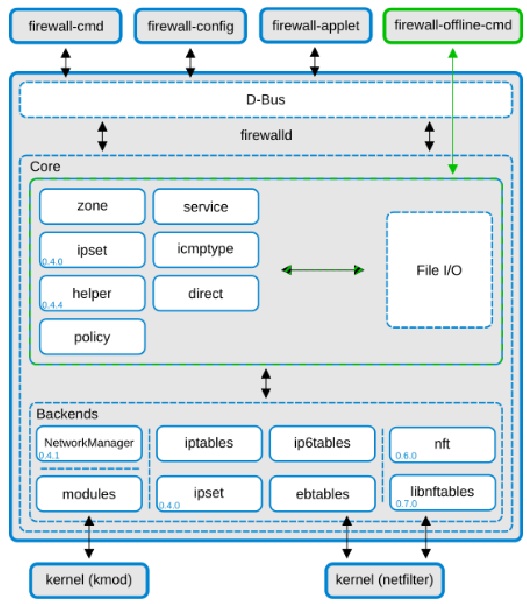
\includegraphics[width=200pt]
        {./graphics/linux/firewalld-architecture.png}
        \caption[Architectuur van firewalld.]{\label{fig:firewalld-architecture}Architectuur van \texttt{firewalld}~\autocite{dakic2022linux}.}
    \end{center}
\end{figure}

Firewalld fungeert echter slechts als een frontend voor \texttt{nftables}~\autocite{dakic2022linux}, een framework dat de netfilter-module van de Linux-kernel vervangt.
Het is ontworpen om de complexiteit van \texttt{iptables} te verminderen.
Zowel \texttt{nftables} als \texttt{iptables} zijn onderdeel van de Linux-kernel, waar ze op kernelniveau netwerkpakketten evalueren aan de hand van de gedefinieerde regels~\autocite{ward2021linux}.

\subsection{Security Enhanced Linux}
\label{linux_selinux}

Security Enhanced Linux, of SELinux, biedt een geavanceerd beveiligingsframework bovenop de standaard Discretionary Access Control (DAC) implementatie van Linux.
DAC vertrouwt namelijk op gebruikers, groepen, en andere rechten om het beveiligingsbeleid van het systeem te bepalen, wat granulariteit mist.

Het is een extra beveiligingslaag die wordt toegevoegd aan de Linux-kernel en standaard aanwezig is op RHEL-gebaseerde systemen.
Echter kan het ook worden ge\"implementeerd op andere Linux-distributies, zoals Debian, maar is het niet standaard ge\"installeerd.

SELinux, of Security Enhanced Linux, voegt een extra laag van beveiliging toe aan Linux-systemen door middel van een Mandatory Access Control (MAC) model, bovenop het standaard Discretionary Access Control (DAC) systeem.
Het onderscheidt zich door unieke beveiligingslabels toe te voegen aan bestanden, processen en andere objecten op het systeem, waardoor het zich richt op beveiligingseigenschappen en abstractie biedt van systeemniveau-details.
Belangrijke elementen van SELinux contexten omvatten gebruiker, rol, type en beveiligingsniveau, waarbij type-informatie cruciaal is voor het handhaven van het beleid.
Deze types, zoals \texttt{httpd\_t} voor de webserver en \texttt{httpd\_sys\_content\_t} voor webserverbestanden, specificeren toegestane interacties tussen processen en bronnen~\autocite{selinux-rhel8}.

SELinux beleidsregels maken gebruik van deze contexten om toegang te beperken en te reguleren.
Bijvoorbeeld, de webserver Apache (\texttt{httpd\_t}) krijgt expliciete toegang tot bestanden in \texttt{/var/www/html/} (\texttt{httpd\_sys\_content\_t}) door middel van een beleidsregel.
Toegang tot andere mappen/ zoals \texttt{/data/mysql/}, wordt echter standaard geweigerd, tenzij specifiek aangegeven, zoals te zien is in figuur~\ref{fig:sleinux-example}~\autocite{selinux-rhel8}.
Deze strikte controle, zelfs in het geval van een gecompromitteerd proces zoals Apache, verhoogt de systeemveiligheid aanzienlijk, waardoor SELinux een krachtig instrument is voor het beveiligen van Linux-systemen.

\begin{figure}[h!]
    \begin{center}
        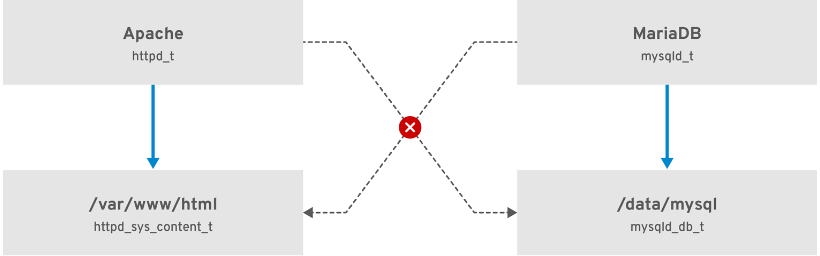
\includegraphics[width=300pt]
        {./graphics/linux/selinux-example.png}
        \caption[Voorbeeld van SELinux werking.]{\label{fig:sleinux-example}Voorbeeld dat de werking van SELinux illustreert. De Apache-webserver kan enkel bestanden aanspreken die zijn gelabeld met het \texttt{httpd\_sys\_content\_t} label, terwijl de MariaDB-database enkel bestanden kan aanspreken die zijn gelabeld met het \texttt{mysqld\_db\_t} label~\autocite{selinux-rhel8}.}
    \end{center}
\end{figure}

\subsection{AppArmor}
\label{linux_apparmor}

In het voorgaande gedeelte is SELinux besproken als een beveiligingsframework dat een Mandatory Access Control (MAC) model implementeert.
Maar SELinux is niet de enige oplossing beschikbaar voor Linux-systemen.
Op Debian-gebaseerde systemen wordt vaak AppArmor gebruikt als een alternatief beveiligingsframework dat vergelijkbare functionaliteit biedt.

AppArmor, wat staat voor Application Armor, is ontworpen om applicaties te beschermen tegen ongeautoriseerde toegang tot het systeem.
Het bereikt dit door het isoleren van onbetrouwbare applicaties en het beperken van hun toegang tot bestanden, directories en andere bronnen.
Deze beperkingen worden ge\"implementeerd via profielen, die de toegestane interacties tussen applicaties en bronnen specificeren~\autocite{gruenbacher2007apparmor}.
Deze profielen worden opgeslagen in de \texttt{/etc/apparmor.d/} directory en kunnen worden aangepast om de beveiliging van het systeem te configureren~\autocite{apparmor-ubuntu}.
Het is echter belangrijk op te merken dat AppArmor zich beperkt tot deze profielen en niet de uitgebreide beveiligingsmogelijkheden biedt die SELinux biedt.

In tegenstelling tot SELinux maakt AppArmor geen gebruik van labels om toegang te beperken, maar gebruikt het paden.
Dit betekent dat als een applicatie toegang heeft tot \texttt{/var/www/html/}, het alleen toegang heeft tot die map en niet tot \texttt{/var/www/} of \texttt{/var/}.
Als we bijvoorbeeld \texttt{/var/www/html/} hernoemen naar \texttt{/var/www/html.backup/}, zal de applicatie geen toegang meer hebben tot die map omdat het pad niet meer overeenkomt met het profiel van de applicatie.
In dat geval moet de beheerder het profiel van de applicatie aanpassen om de nieuwe locatie toe te staan~\autocite{gruenbacher2007apparmor}.

%%=============================================================================
%% Netwerkconcepten
%%=============================================================================

\chapter{\IfLanguageName{dutch}{Computernetwerk concepten}{Computer network concepts}}%
\label{ch:computernetwerk-concepten}

\section{Inleiding}
\label{netwerk_inleiding}

Tegenwoordig heeft vrijwel elke server toegang nodig tot het netwerk om te kunnen communiceren met andere servers of clients.
Dit vormt een essentieel onderdeel van de serverfunctionaliteit, aangezien het zonder netwerkconnectiviteit niet bereikbaar zou zijn.
Om deze connectiviteit te realiseren, zijn er verschillende concepten en technologie\"en beschikbaar die kunnen worden toegepast.

In dit hoofdstuk zullen we enkele van deze concepten en technologie\"en bespreken die ons later zullen helpen bij het identificeren van wat het beste kan worden opgenomen in ons configuratie-inventaris.

\section{Netwerkinterface}
\label{netwerk_netwerkinterface}

Een netwerkinterfacecontroller (NIC) is een hardwarecomponent die een computer in staat stelt te communiceren met andere computers via een netwerk.
Het bereidt de gegevens voor die moeten worden verzonden en ontvangen, en zet deze om naar een formaat dat via het netwerk kan worden verzonden.
Een systeem kan meerdere NIC's bevatten; bijvoorbeeld een laptop kan zowel een draadloze NIC voor WiFi als een bedrade NIC voor Ethernet hebben~\autocite{hypponen2021securing}.
Binnen het OSI-model maakt de NIC deel uit van de fysieke laag.

Voordat een NIC kan worden gebruikt, moet de juiste netwerkdriver zijn geïnstalleerd op het systeem.
Deze driver stuurt de onderliggende hardware aan en zorgt ervoor dat deze correct communiceert met het besturingssysteem.
Daarnaast is de driver verantwoordelijk voor het toewijzen van adressen, het aanpassen van transmissieparameters en het waarborgen van het netwerkverkeer~\autocite{hypponen2021securing}.

\section{Netwerkprotocollen}
\label{netwerk_netwerkprotocollen}

Netwerken zijn bijna altijd hi\"erarchisch opgebouwd en bestaan uit verschillende lagen.
Elke laag heeft zijn eigen specifieke functie en is verantwoordelijk voor een bepaald aspect van de communicatie.
Het OSI-model (Open Systems Interconnection model) is een referentiemodel dat deze lagen beschrijft en de communicatie tussen systemen mogelijk maken.
Dit model heeft de volgende lagen~\autocite{tanenbaum1981network}:

\begin{enumerate}
    \item Fysieke laag
    \item Data link laag
    \item Netwerklaag
    \item Transportlaag
    \item Sessielaag
    \item Presentatielaag
    \item Applicatielaag
\end{enumerate}

Dit deel zullen enkele van de belangrijkste protocollen en technologie\"en worden besproken die worden gebruikt in computernetwerken.

\subsection{Internet Protocol versie 4}
\label{netwerk_ipv4}

IPv4, voluit het Internet Protocol versie 4 genoemd, is de vierde iteratie van het Internet Protocol en wordt ingezet op de netwerklaag van het OSI-model, als onderdeel van de TCP/IP-protocolstack.
Dit protocol, ontworpen door DARPA (Defense Advanced Research Projects Agency), is momenteel het meest gangbare Internet Protocol.
Het vormt de ruggengraat van het internet en faciliteert de verzending van pakketten van de ene computer naar de andere, via een reeks van onderling verbonden netwerken.

In de werking van het protocol worden gegevens van de bovenliggende lagen ge\"encapsuleerd in pakketten, die vervolgens over het netwerk worden verzonden.
Samen met de IPv4-header, die metadata bevat over het pakket, worden de gegevens doorgegeven van netwerk naar netwerk, totdat ze hun bestemming bereiken of de maximale levensduur bereiken (aangeduid als TTL, oftewel Time to Live, zoals te zien in figuur~\ref{fig:network-ipv4-header}).
Wanneer de TTL is verstreken, wordt het pakket verwijderd en wordt er een ICMP-pakket teruggestuurd naar de afzender om dit aan te geven~\autocite{dordal2020}.

\begin{figure}[h!]
    \begin{center}
        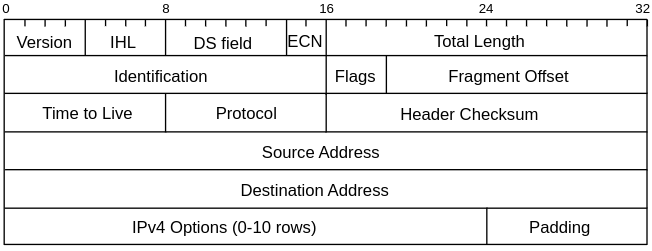
\includegraphics[width=300pt]
        {./graphics/network/ipv4-header.png}
        \caption{\label{fig:network-ipv4-header}Diagram van een IPv4 header~\autocite{dordal2020}.}
    \end{center}
\end{figure}

Ipv4 maakt gebruik van 32-bit adressen en ondersteunt ongeveer \(2^{32}\) adressen, wat neerkomt op ongeveer 4,3 miljard unieke adressen.
Een adres wordt gelinkt aan een specifieke netwerkinterface en maakt het mogelijk om deze interface te identificeren en te lokaliseren binnen een netwerk.
Wanneer we spreken over een IPv4-adres, verwijzen we meestal naar een van de volgende notaties:

\begin{itemize}
    \item \texttt{192.168.0.82}
    \item \texttt{127.0.0.1}
\end{itemize}

Dit zijn zogenaamde dotted-decimal notaties, waarbij elk octet van het adres wordt gescheiden door een punt.
Als we echter een adres in een binair formaat willen weergeven, kunnen we dit doen door elk octet te converteren naar een 8-bit binair getal en deze aan elkaar te koppelen.
Dit resulteert in volgende notatie, respectievelijk voor de bovenstaande voorbeelden:

\begin{itemize}
    \item \texttt{11000000.10101000.00000000.01010010}
    \item \texttt{01111111.00000000.00000000.00000001}
\end{itemize}

Deze IP-adressen kunnen we verdelen in twee delen: het netwerkdeel en het hostdeel.
Neem bijvoorbeeld het adres \texttt{192.168.0.82}, dat we kunnen opsplitsen in \texttt{192.168.0} en \texttt{82}.
Deze scheiding is nuttig om vast te stellen welke hosts zich in hetzelfde netwerk bevinden en welke niet.
De splitsing wordt bepaald door een subnetmask, dat aangeeft welke bits van het adres het netwerkdeel vormen en welke het hostdeel.
In het geval van \texttt{192.168.0.82} zou het subnetmask bijvoorbeeld \texttt{255.255.255.0} zijn, wat overeenkomt met 24 bits voor het netwerkdeel en 8 bits voor het hostdeel.
Een andere notatie die wordt gebruikt, is de CIDR-notatie, waarbij het aantal bits dat het netwerkdeel vormt direct wordt aangegeven.
Voor het bovenstaande voorbeeld zou dit \texttt{192.168.0.82/24} zijn.

\subsection{Internet Protocol versie 6}
\label{netwerk_ipv6}

IPv6, oftewel Internet Protocol versie 6, vertegenwoordigt de opvolging van IPv4 en is ontworpen om de beperkingen van zijn voorganger aan te pakken.
Met de exponenti\"ele groei van het internet en de groeiende vraag naar meer adressen werd duidelijk dat het beschikbare aantal IPv4-adressen ontoereikend zou zijn.
Als reactie hierop werd IPv6 ontwikkeld, dat gebruikmaakt van 128-bit adressen en naar schatting ongeveer \(2^{128}\) unieke adressen ondersteunt.

Dit protocol functioneert op de netwerklaag van het OSI-model en vertoont overeenkomsten met IPv4 in termen van werking.
Het onderscheidt zich echter door zijn adressering, die in een andere notatie wordt weergegeven en meer bits bevat.
Bovendien bestaat de header van een IPv6-pakket uit 40 bytes, wat tweemaal zo groot is als de 20 bytes van een IPv4-header, zoals geïllustreerd in figuur~\ref{fig:network-ipv6-header}~\autocite{dordal2020}.

\begin{figure}[h!]
    \begin{center}
        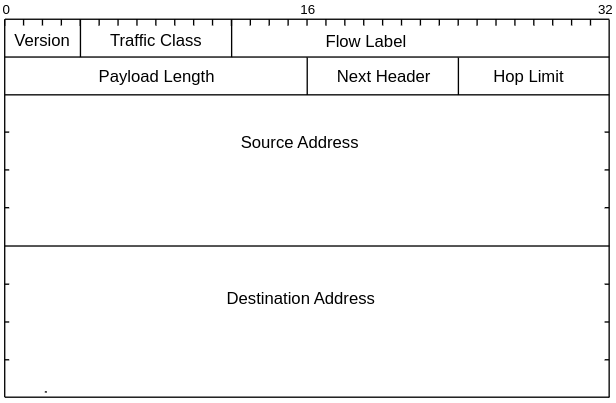
\includegraphics[width=300pt]
        {./graphics/network/ipv6-header.png}
        \caption{\label{fig:network-ipv6-header}Diagram van een IPv6 header~\autocite{dordal2020}.}
    \end{center}
\end{figure}

De IPv6-header verschilt van zijn IPv4-tegenhanger. Zo ontbreekt bijvoorbeeld het TTL-veld en wordt dit vervangen door een veld genaamd Hop Limit.

IPv6 maakt gebruik van adressen die 128 bits lang zijn en worden weergegeven in een hexadecimale notatie, zoals in het volgende voorbeeld:

\begin{itemize}
    \item \texttt{fe80::7255:7ef:9d20:a8ae}
    \item \texttt{::1} (IPv6 equivalent van \texttt{127.0.0.1})
\end{itemize}

\subsection{Routingtabellen}
\label{netwerk_routeringstabel}

Het doorsturen van pakketten van de ene host naar de andere gebeurt via routers, die fungeren als tussenstations in het netwerk.
Deze routers houden elk hun eigen routingtabel bij, ook wel bekend als een IP-forwardingtabel~\autocite{dordal2020}.
Computers houden zelf ook een routingtabel bij om te bepalen naar welke router ze pakketten moeten sturen om hun bestemming op een zo efficiënt mogelijke manier te bereiken, zoals te zien is in listing~\ref{lst:linux-routering}.

\begin{listing}
  \begin{minted}[linenos,tabsize=4,breaklines]{console}
[anton@fedorable ~]$ ip route
default via 192.168.0.1 dev wlo1 proto dhcp src 192.168.0.82 metric 600
192.168.0.0/24 dev wlo1 proto kernel scope link src 192.168.0.82 metric 600
  \end{minted}
  \caption{Uitvoer van het commando \texttt{ip route} op een Linux-systeem, dat de routeringstabel toont.}
  \label{lst:linux-routering}
\end{listing}

Zoals te zien is in listing~\ref{lst:linux-routering}, bevat de routingtabel routes naar specifieke netwerken, die elk een doeladres en een netwerkinterface bevatten.
Op basis hiervan wordt een pakket doorgestuurd naar de juiste router, die het vervolgens verder doorstuurt naar de volgende router of naar de bestemming.
IP-forwardingtabellen bevatten netwerkvoorvoegsels als bestemmingen, zoals beschreven in de tekst.
Het matchen van een pakketadres met een vermelding in de forwardingtabel vereist vergelijking van de voorvoegsels, niet alleen eenvoudige gelijkheidscontrole.

\subsection{User Datagram Protocol}
\label{netwerk_udp}

UDP, voluit User Datagram Protocol, is een ander protocol dat, net als TCP, opereert op de transportlaag van het OSI-model.
Het onderscheidt zich doordat het een eenvoudig protocol is dat communicatie mogelijk maakt tussen twee hosts zonder dat er eerst een verbinding hoeft te worden opgezet.
Dit betekent dat het een connectionless protocol is, in tegenstelling tot TCP, waarover we later zullen praten.

Het staat bekend als een lichtgewicht protocol dat snel en effici\"ent werkt, maar geen garanties biedt voor de levering van pakketten.
Wanneer een zender een pakket naar de ontvanger stuurt, is er geen bevestiging van ontvangst, wat betekent dat pakketten verloren kunnen gaan zonder dat de zender hiervan op de hoogte is.

UDP communiceert op basis van datagrammen, die onafhankelijk van elkaar worden verzonden en ontvangen.
Binnen elk datagram is er een header van 8 bytes aanwezig, die is onderverdeeld in vier gelijke velden van elk 16 bits.
De eerste 16 bits vertegenwoordigen de bronpoort, die waarden kan hebben tussen 0 en 65535 en applicaties identificeert.
Het tweede deel van de header bevat de doelpoort, die eveneens varieert van 0 tot 65535 en de bestemmingsapplicatie identificeert.
Vervolgens is er een veld van 16 bits voor de lengte van het datagram en een checksum van 16 bits om de integriteit van het pakket te waarborgen~\autocite{dordal2020}.
Een voorbeeld van een UDP-header is te zien in figuur~\ref{fig:netwerk-udp-header}.

\begin{figure}[h!]
    \begin{center}
        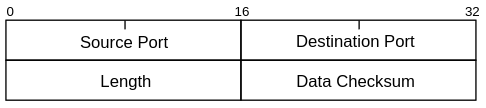
\includegraphics[width=200pt]
        {./graphics/network/udp-header.png}
        \caption{\label{fig:netwerk-udp-header}Diagram van een UDP header~\autocite{dordal2020}.}
    \end{center}
\end{figure}

\subsection{Transmission Control Protocol}
\label{netwerk_tcp}

Net als UDP is TCP, staande voor Transmission Control Protocol, een essentieel protocol voor communicatie tussen hosts op een netwerk.
Toch verschillen de twee protocollen in hoe ze gegevens verzenden en ontvangen.
In tegenstelling tot UDP is TCP een connection-oriented protocol, wat betekent dat het eerst een verbinding opzet voordat gegevens worden uitgewisseld.
Dit gebeurt via de zogenaamde three-way handshake, waarbij beide partijen communiceren om ervoor te zorgen dat gegevens correct en in de juiste volgorde worden afgeleverd.

Om communicatie via TCP mogelijk te maken, stuurt een van de hosts een SYN-pakket naar de andere host.
Wanneer de ontvangende host dit pakket ontvangt, stuurt deze een SYN-ACK-pakket terug naar de zender.
Vervolgens stuurt de zender een ACK-pakket terug, waarna de verbinding tot stand is gebracht en gegevens kunnen worden uitgewisseld.
Dit proces wordt geïllustreerd in figuur~\ref{fig:netwerk-tcp-handshake}~\autocite{hypponen2021securing}.

\begin{figure}[h!]
    \begin{center}
        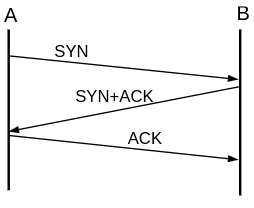
\includegraphics[width=100pt]
        {./graphics/network/tcp-handshake.png}
        \caption{\label{fig:netwerk-tcp-handshake}TCP three-way handshake~\autocite{dordal2020}.}
    \end{center}
\end{figure}

De TCP-header is ook complexer dan die van UDP, met een totale lengte van 20 bytes, zoals weergegeven in figuur~\ref{fig:netwerk-tcp-header}.
Net als bij UDP beginnen de bron- en doelpoorten de header, die vari\"eren van 0 tot 65535.
Daarna volgt een veld voor de sequentienummering, dat de volgorde van de gegevens bepaalt.
Verder is er een veld voor de bevestigingsnummering, dat wordt gebruikt om te bevestigen dat gegevens correct zijn ontvangen.
Ook bevat de header weer een checksum om de integriteit van het pakket te waarborgen~\autocite{dordal2020}.

\begin{figure}[h!]
    \begin{center}
        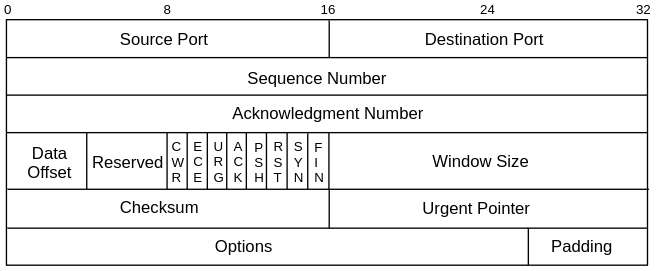
\includegraphics[width=300pt]
        {./graphics/network/tcp-header.png}
        \caption{\label{fig:netwerk-tcp-header}Diagram van een TCP header~\autocite{dordal2020}.}
    \end{center}
\end{figure}

\subsection{Domain Name System}
\label{netwerk_dns}

Eerder werd al benadrukt dat elke host op een netwerk minstens één IP-adres heeft.
Hoewel deze IP-adressen essentieel zijn voor communicatie op internet, zijn ze niet bijzonder gebruiksvriendelijk.
Het onthouden en gebruiken van lange reeksen cijfers is niet praktisch in het dagelijks gebruik.
Om deze uitdaging aan te pakken en het internet toegankelijker te maken, is het Domain Name System (DNS) ontwikkeld.

Het hele protocol zou men kunnen vergelijken met een telefoonboek, waarbij domeinnamen worden vertaald naar IP-adressen en omgekeerd.
Gelijkaarig aan een telefoonboek waar we de namen van personen kunnen opzoeken en hun telefoonnummer kunnen vinden, kunnen we met DNS de IP-adressen van domeinnamen opzoeken.

De structuur van DNS is hi\"erarchisch van aard, waarbij domeinnamen worden opgedeeld in verschillende niveaus.
Neem bijvoorbeeld het domein \texttt{www.google.com}. Dit wordt opgedeeld in drie niveaus: \texttt{www}, \texttt{google}, en \texttt{com}.
Deze hi\"erarchische structuur maakt het mogelijk om domeinnamen logisch te organiseren en effici\"ent te beheren~\autocite{dordal2020}.

Wanneer een host een DNS-query uitvoert om een domeinnaam om te zetten naar een IP-adres, raadpleegt deze een DNS-server.
De DNS-server heeft een enorme database met domeinnamen en hun bijbehorende IP-adressen.
De host stuurt een verzoek naar de DNS-server, vraagt om de vertaling van een specifieke domeinnaam en ontvangt vervolgens het bijbehorende IP-adres als reactie.
Op deze manier kan een host bijvoorbeeld een verzoek sturen naar een DNS-server om het IP-adres van \texttt{www.google.com} te verkrijgen, waarna de DNS-server het IP-adres \texttt{142.251.39.110} teruggeeft, zoals aangetoond in listing~\ref{lst:dns-query}.
Dit IP-adres kan dan worden gebruikt om verbinding te maken met de betreffende website.

\begin{listing}
  \begin{minted}[linenos,tabsize=4,breaklines]{console}
[anton@fedorable ~]$ nslookup google.com
Server:         127.0.0.53
Address:        127.0.0.53#53

Non-authoritative answer:
Name:   google.com
Address: 142.251.39.110
Name:   google.com
Address: 2a00:1450:400e:811::200e
  \end{minted}
  \caption{Voorbeeld van een DNS-query met behulp van het \texttt{nslookup} commando.}
  \label{lst:dns-query}
\end{listing}

%%=============================================================================
%% Methodologie
%%=============================================================================

\chapter{\IfLanguageName{dutch}{Het opstellen van een configuratie-inventaris}{The creation of a configuration inventory}}
\label{ch:risicoanalyse}

\section{Inleiding}
\label{risico_inleiding}

De overgang van een traditionele omgeving naar een Infrastructure as Code (IaC) omgeving vereist een grondige kennis van de configuratie van Linux-systemen.
Een cruciale stap in dit proces is het opstellen van een gedetailleerde configuratie-inventaris die alle essenti\"ele eigenschappen van het systeem omvat.
Deze inventaris vormt de basis voor het automatiseren van de infrastructuur met behulp van IaC-tools zoals Ansible, Terraform of Puppet.
In dit hoofdstuk zal men de belangrijkste elementen bespreken die moeten worden opgenomen in een configuratie-inventaris van Linux-systemen voor een succesvolle overgang naar een IaC-omge-\ ving, waarbij men ook de relevante beveiligingsaspecten benadrukken.

\section{Het besturingssysteem}
\label{risico_besturingssysteem}

Een eerste stap bij het opstellen van een configuratie-inventaris is het verzamelen van basisinformatie over het Linux-systeem.
Dit omvat details zoals het besturingssysteem (bijvoorbeeld Debian, Ubuntu, CentOS), de versie van de kernel, en de hardware-specificaties zoals CPU-model, geheugen en opslagcapaciteit.
Het is essentieel om deze informatie vast te leggen om een goed beeld te krijgen van de huidige configuratie van het systeem.

Uit~\ref{linux_linux_besturingssysteem}, bleek dat de kernel een cruciaal onderdeel is van het besturingssysteem en een directe impact heeft op de beveiliging en prestaties van het systeem.
Hierdoor is het belangrijk om kernel die op dit moment gebruikt wordt, te documenteren in de configuratie-inventaris, alsook alle kernel-modules die momenteel geladen zijn.
Ook de versie van het besturingssysteen is van belang, omdat verschillende versies van Linux-distributies verschillende pakketten en configuraties kunnen bevatten.

\subsection{Gebruikers- en groepsbeheer}
\label{risico_gebruikers_groepen}

Het beheren van gebruikers en groepen vormt een essentieel aspect van systeemconfiguratie.
Dit is van cruciaal belang omdat gebruikers vaak worden aangemaakt om specifieke taken uit te voeren, zoals bijvoorbeeld de \texttt{www-data} gebruiker die doorgaans wordt gebruikt voor het beheer van de Apache webserver, zoals besproken in~\ref{linux_gebruikers_groepen}.
In de configuratie-inventaris moeten alle gebruikersaccounts en groepen op het systeem worden opgenomen, inclusief hun respectievelijke rechten en permissies.
Dit omvat ook informatie over speciale gebruikersaccounts zoals de rootgebruiker, systeemgebruikers en de geconfigureerde \texttt{sudo}-rechten van elke gebruiker.

Door deze gegevens op te nemen in de configuratie-inventaris, kan men later controleren welke gebruikers en groepen daadwerkelijk op het systeem aanwezig moeten zijn om de vereiste taken uit te voeren, en welke niet.
Door de geregistreerde \texttt{sudo}-regels te analyseren, kan men bepalen of een bepaalde gebruiker over de juiste machtigingen beschikt, of dat het beter is om het aantal permissies te beperken.

\subsection{Bestandssysteem en partities}
\label{risico_bestandsysteem_partities}

Bij het installeren of updaten van een systeem is het essentieel om aandacht te besteden aan de opslagmedia, en hun configuratie.
Dit omvat onder andere het kiezen van het juiste bestandssysteem, het configureren van partities en het bepalen van de mountpoints~\autocite{wirzenius1993linux}.
Een grondig begrip van de bestaande bestandssystemen, partities en hun mountpoints is daarom van groot belang.

Dit belang wordt ook benadrukt in het boek "IT Inventory and Resource Management with OCS Inventory" van Barzan ``Tony'' Antal~\autocite{Antal2010}.
De auteur benadrukt welke systeemeigenschappen cruciaal zijn om op te nemen in een configura-\ tie-inventaris.
Hoewel het boek niet specifiek gericht is op Linux-systemen, zijn de principes die worden besproken van toepassing op Linux-omgevingen.

Het is eveneens een optie om back-ups te maken van essenti\"ele bestanden en directories, zoals de \texttt{/etc/} directory waar belangrijke configuratiebestanden worden bewaard.
Andere directories die het waard zijn om te monitoren, zijn onder meer \texttt{/bin/}, \texttt{/sbin/}, \texttt{/usr/bin/} en \texttt{/usr/sbin/}, aangezien deze cruciale systeemprogramma's bevatten~\autocite{linuxfoundation-filesystem}.
Een volgende stap zou zijn om een hash te berekenen van deze bestanden en deze hash vervolgens op te nemen in de configuratie-inventaris.
Dit kan worden gedaan met behulp van een tool zoals \texttt{sha256sum} om de hash van een bestand te genereren.

Een andere handige tool die ons kan ondersteunen in dit, is Wazuh, een krachtige Security Information and Event Management (SIEM) die ons in staat stelt om onze infrastructuur te monitoren, variërend van servers tot gewone werkstations.
Naast File Integrity Monitoring (FIM) biedt Wazuh ook mogelijkheden voor Security Configuration Assessment (SCA), waardoor systeemconfiguraties worden versterkt tegen potentiële bedreigingen.
Bovendien omvat het kwetsbaarheidsdetectie, waarmee potentiële zwakke punten kunnen worden geïdentificeerd voordat ze worden misbruikt~\autocite{wazuh-overview}.

Het toepassen van hashberekeningen draagt bij aan een verhoogde integriteit van de data, aangezien het ons de mogelijkheid biedt om te controleren of de bestanden zijn gewijzigd.
Immers, de hash van een bestand verandert wanneer de inhoud van het bestand wijzigt.
Bovendien is het belangrijk om te vermelden dat hashfuncties one-way zijn, wat betekent dat het niet mogelijk is om de originele inhoud van het bestand te herstellen aan de hand van de hash~\autocite{herrero2021file}.

Een praktisch voorbeeld van het gebruik van \texttt{sha256sum} om de hash van bestanden te berekenen, wordt gedemonstreerd in listing~\ref{lst:sha256sum}.
Hier kan men zien dat er drie directories zijn: \texttt{a}, \texttt{b} en \texttt{c}, met in \texttt{a} en \texttt{c} een bestand genaamd \texttt{a.txt}, en in \texttt{b} een bestand genaamd \texttt{b.txt}.
Het resultaat van \texttt{sha256sum} op de bestanden toont dat \texttt{a.txt} in \texttt{a} en \texttt{c} dezelfde hashwaarde heeft, wat aangeeft dat de bestanden identiek zijn, \texttt{b.txt} in \texttt{b} heeft een andere hashwaarde, wat aangeeft dat het bestand verschilt van de andere twee.
Dit geeft aan dat de hashwaarden onafhankelijk zijn van de bestandslocatie, en dat ze een unieke identificatie vormen voor de inhoud van het bestand.

\begin{listing}
  \begin{minted}[linenos,tabsize=4,breaklines]{console}
[anton@fedorable ~]$ find {a,b,c}/ -type f -exec sha256sum {} \;
87428fc522803d31065e7bce3cf03fe475096631e5e07bbd7a0fde60c4cf25c7  a/a.txt
0263829989b6fd954f72baaf2fc64bc2e2f01d692d4de72986ea808f6e99813f  b/b.txt
87428fc522803d31065e7bce3cf03fe475096631e5e07bbd7a0fde60c4cf25c7  c/a.txt
  \end{minted}
  \caption[Find-commando voor bestandshashes.]{Uitvoer van het \texttt{find}-commando om bestanden te vinden en de hash ervan te berekenen met \texttt{sha256sum}.}
  \label{lst:sha256sum}
\end{listing}

\section{Software-installaties en -configuraties}
\label{risico_software}

De nodige software-installaties op een systeem kunnen vari\"eren afhankelijk van de specifieke vereisten van de toepassingen die op het systeem worden uitgevoerd.
Dit kan verschillende cruciale aspecten omvatten, zoals de ge\"installeerde software en de bijbehorende pakketten, evenals de configuratie van deze software.
Een grondige evaluatie en documentatie van de ge\"installeerde software en de bijbehorende pakketten, alsook hun configuratie, is essentieel voor een succesvolle overgang naar een IaC-omgeving.

\subsection{Ge{\"i}nstalleerde applicaties en bronnen}
\label{risico_software_installaties_bronnen}

Een grondig begrip van de ge\"installeerde software en de bijbehorende pakketten is essentieel voor een succesvolle overgang naar een IaC-omgeving en is ook van cruciaal belang op het gebied van beveiliging.
Het vastleggen van deze informatie in de configuratie-inventaris is noodzakelijk voor een effectieve beveiligingsstrategie.

De configuratie-inventaris moet een gedetailleerde lijst bevatten van alle ge\"installeerde softwarepakketten, inclusief hun versies en afhankelijkheden, evenals informatie over de bronnen waaruit de software is ge\"installeerd.
Dit omvat zowel systeemniveau-software als gebruikersniveau-toepassingen.
Het verzamelen van deze informatie kan worden uitgevoerd met behulp van package managers zoals \texttt{dpkg} of \texttt{rpm} om een lijst van ge\"installeerde pakketten te genereren.
Ook moeten de geconfigureerde repositories worden opgenomen in de configuratie-inventaris, aangezien deze de bron zijn voor vele software-installaties.

Een treffend voorbeeld dat illustreert waarom dit zo belangrijk is, betreft CVE-2024-3094~\autocite{nist-CVE-2024-3094}.
Deze backdoor werd ontdekt in maart 2024, in de veelgebruikte software genaamd \texttt{xz-utils}, een standaard compressie- en decompressietool, dat deel uitmaakt van de \texttt{liblzma}-biblio-\ theek.
Deze bibliotheek wordt vaak gebruikt op Linux-systemen door andere programma's.
Het werd opgemerkt nadat Andres Freund, een softwareontwikkelaar, verdachte code had gevonden in de broncode van het pakket.
Echter bleek de backdoor alleen aanwezig te zijn in versies 5.6.0 en 5.6.1 van de software, die werden uitgebracht in februari 2024~\autocite{lins2024critical}.
Op dat moment waren de ge\"infecteerde versies beschikbaar in de repositories van verschillende Linux-distributies, waaronder Debian (testing en unstable), Alpine Linux (Edge) en Fedora (40, 41 en Rawhide).

\subsection{Configuratie van ge{\"i}nstalleerde software}
\label{risico_software_configuratie}

Met enkel en alleen de ge\"installeerde software te documenteren, is het echter niet voldoende, aangezien het later de bedoeling is om aan de hand van dit inventaris een IaC-omgeving op te zetten.
Voor een volledige overgang naar een IaC-omgeving is het ook noodzakelijk om de huidige configuratie van de software vast te leggen, zodat men deze later kan omvormen naar code voor de gekozen IaC-tool.

Op Linux-systemen worden configuratiebestanden vaak bewaard in de \texttt{/etc/} directory, afgeleid van ``et cetera''~\autocite{linuxfoundation-filesystem}.
De bestanden in deze directory bevatten vaak de configuratie-opties voor verschillende softwarepakketten, en het is mogelijk om deze bestanden op te nemen in een configuratie-inventaris.

\subsection{Taakbeheer}
\label{risico_taakbeheer}

Systemd werd reeds besproken in~\ref{linux_systemd} als de standaard init-systeem op de meeste Linux-distributies.
Het is een manier om services, en processen, te starten en stoppen op een bepaald tijdstip, of bij een bepaalde gebeurtenis.
Zo kan men bijvoorbeeld een webserver automatisch laten starten bij het opstarten van het systeem.
Dit doet men met het \texttt{systemctl} commando gevolgd door de \texttt{enable} optie, zoals te zien in listing~\ref{lst:systemd_enable}.

\begin{listing}
  \begin{minted}[linenos,tabsize=4,breaklines]{console}
[root@fedorable ~]$ systemctl enable sshd
Created symlink /etc/systemd/system/multi-user.target.wants/sshd.service → /usr/lib/systemd/system/sshd.service.
  \end{minted}
  \caption[Automatische service start met systemctl.]{Uitvoer van het \texttt{systemctl}-commando om een service automatisch te laten starten bij het opstarten van het systeem.}
  \label{lst:systemd_enable}
\end{listing}

Doordat systemd units vaak worden gebruikt om services te beheren, is het van belang om deze units op te nemen in de configuratie-inventaris.
Net zoals het bijhouden van een lijst van services die automatisch worden gestart bij het opstarten van het systeem, dit kan worden bereikt door \texttt{systemctl} te gebruiken met de \texttt{list-unit-files} optie, zoals te zien in listing~\ref{lst:systemd_list_unit_files}.

\begin{listing}
  \begin{minted}[linenos,tabsize=4,breaklines]{console}
[root@fedorable ~]$ systemctl list-unit-files --state=enabled
UNIT FILE                          STATE   PRESET
cups.path                          enabled enabled
abrt-journal-core.service          enabled enabled
abrt-oops.service                  enabled enabled
abrt-vmcore.service                enabled enabled
abrt-xorg.service                  enabled enabled
[...]
  \end{minted}
  \caption[Lijst van automatisch gestarte services.]{Uitvoer van het \texttt{systemctl}-commando om een lijst van services te tonen die automatisch worden gestart bij het opstarten van het systeem.}
  \label{lst:systemd_list_unit_files}
\end{listing}

Verder werd in~\ref{linux_cronjobs} besproken dat cronjobs worden gebruikt om taken op een gepland tijdstip uit te voeren.
Dit zou kunnen gebruikt worden als alternatief voor systemd timers, daarom is het ook hier belangrijk om deze cronjobs op te nemen in de configuratie-inventaris.
Dit zou men kunnen bereiken door een kopie te maken van de directories \texttt{/etc/cron.d/}, \texttt{/etc/cron.daily/}, \texttt{/etc/cron.hourly/}, \texttt{/etc/cron.monthly/} en \texttt{/etc/cron.weekly/}, alsook \texttt{/etc/crontab} die alle cronjobs bevat.

\section{Netwerkconfiguratie}
\label{risico_netwerkconfiguratie}

Vele Linux-systemen maken gebruik van netwerkverbindingen om te communiceren met andere systemen en diensten.
Dit werd reeds besproken in~\ref{ch:computernetwerk-concepten}, waarbij de basisprincipes van computernetwerken werden toegelicht, alsook enkele protocollen die worden gebruikt voor netwerkcommunicatie.
Een basis oplijsting van de netwerkconfiguratie is essentieel voor een succesvolle overgang naar een IaC-omgeving, omdat het de basis vormt voor de netwerkautomatisering.
Ook zorgt het opnemen van de netwerkconfiguratie in de configuratie-inventaris ervoor dat men een begrip heeft over welke systemen met elkaar kunnen communiceren en welke niet.

\subsection{Netwerkinterfaces}
\label{risico_netwerkinterfaces}

In~\ref{netwerk_netwerkinterface} heeft men al besproken dat netwerkinterfaces de fysieke of virtuele verbindingen zijn waardoor een Linux-systeem communiceert met andere systemen.
Elke interface heeft een IP-adres, of het nu IPv4 of IPv6 is, samen met een subnetmask en een gateway.
Deze kenmerken stellen het systeem in staat om uniek ge\"identificeerd te worden binnen het netwerk.

Het is daarom van groot belang om de netwerkinterfaces op te nemen in de confi-\ guratie-inventaris, inclusief hun configuratiegegevens zoals het IP-adres, subnetmask en gateway.
Of het nu gaat om een interface die zijn instellingen verkrijgt via DHCP of handmatig is geconfigureerd, het vastleggen van deze informatie is van cruciaal belang.

Wanneer een IP-adres wordt verkregen via een DHCP-lease, is ook informatie over de DHCP-server relevant.
Dit omvat niet alleen het IP-adres van de server, maar ook de lease-tijd en eventuele configuratieopties die door de server aan het systeem zijn verstrekt.
Zoals aangegeven door Antal in het boek ``It Inventory and Resource Management with OCS Inventory''~\autocite{Antal2010}, is het vastleggen van deze informatie essentieel voor het beheer van de netwerkconfiguratie.

\subsection{Routing en poortbeheer}
\label{risico_routing_poorten}

In hoofdstuk~\ref{ch:computernetwerk-concepten} heeft men al besproken hoe routing en poortbeheer cruciale elementen zijn binnen netwerkconfiguratie.
Poorten worden gebruikt om applicaties met andere systemen te laten communiceren, terwijl routing ervoor zorgt dat het verzonden verkeer zijn bestemming bereikt.

Het documenteren van de momenteel gebruikte poorten in de configuratie-inven-\ taris biedt inzicht in de communicatiekanalen die actief zijn.
Dit stelt beheerders in staat om een volledig overzicht te hebben van welke applicaties welke poorten gebruiken, wat van onschatbare waarde is bij het beheren en beveiligen van het netwerk.

Bij het bekijken van de routingtabel is het van essentieel belang om de huidige routingconfiguratie vast te leggen.
Dit omvat niet alleen de standaardgateway, maar ook eventuele statische routes die zijn geconfigureerd op het systeem.
Het vastleggen van deze informatie zorgt ervoor dat het verkeer effici\"ent wordt geleid naar de juiste bestemmingen, wat de algehele netwerkprestaties en betrouwbaarheid ten goede komt.

\subsection{DNS-configuratie}
\label{risico_dns}

DNS speelt een cruciale rol in het vertalen van domeinnamen naar IP-adressen, zoals besproken in~\ref{netwerk_dns}.
Een goed functionerend netwerk vereist dan ook een nauwkeurige DNS-configuratie, omdat deze ervoor zorgt dat systemen correct kunnen communiceren met andere systemen en diensten.
Daarom is het van groot belang om de DNS-configuratie vast te leggen in de configuratie-inventaris.

Naast het operationele belang is het documenteren van de DNS-configuratie ook vanuit een beveiligingsperspectief essentieel.
Door deze informatie te registreren, kunnen beheerders controleren welke DNS-servers momenteel worden gebruikt en kunnen ze beoordelen of deze veilig zijn.
Dit is van cruciaal belang om aanvallen zoals DNS-hijacking te voorkomen, waarbij een aanvaller de controle over een DNS-server overneemt om verkeer om te leiden naar kwaadaardige websites door de DNS-records op de server te wijzigen~\autocite{shaikh2020overcoming}.
Het proactief documenteren van de DNS-configuratie stelt beheerders in staat om potenti\"ele beveiligingsrisico's te identificeren en te vermijden, waardoor de algehele veiligheid van het netwerk wordt versterkt.

\section{Beveiligingsconfiguratie}
\label{risico_beveiligingsconfiguratie}

De overgang van een traditionele omgeving naar een Infrastructure as Code (IaC) omgeving brengt verschillende belangrijke aspecten met zich mee, met name op het gebied van beveiliging.
Deze overgang vereist een zorgvuldige herziening en documentatie van de beveiligingsmaatregelen om ervoor te zorgen dat de IaC-omgeving dezelfde, zo niet betere, beveiligingsniveaus biedt dan de voorafgaande traditionele omgeving.

\subsection{Firewall}
\label{risico_firewall}

Een van de pijlers van Linux-serverbeveiliging is de firewall, die inkomend en uitgaand verkeer reguleert om ongewenste toegang tot het systeem te voorkomen.
Bij de overgang naar IaC is het noodzakelijk om de configuratie van de firewall, zoals beheerd door \texttt{firewalld} of \texttt{nftables}, gedetailleerd te documenteren.
Dit omvat het defini\"eren van toegestane en geblokkeerde poorten, services en zones, evenals eventuele aangepaste regels die zijn geconfigureerd om specifieke beveiligingsvereisten te vervullen.

\subsection{SELinux}
\label{risico_selinux}

Naast de firewall is SELinux een cruciaal onderdeel van Linux-serverbeveiliging, met zijn Mandatory Access Control (MAC) model dat extra bescherming biedt bovenop de standaard Discretionary Access Control (DAC) implementatie.
Bij de overgang naar een IaC-omgeving is het van vitaal belang om de SELinux-configuratie op te nemen in de inventaris.
Dit omvat het documenteren van de SELinux-policy's, contexten en beleidsregels die van toepassing zijn op verschillende systeembronnen en processen.
Door de SELinux-configuratie te documenteren, kan het IaC-proces deze beveiligingsmaatregelen automatiseren en consistent toepassen op alle servers in de omgeving.

\subsection{AppArmor}
\label{risico_apparmor}

Hoewel SELinux de standaard is voor beveiligingsbeleid op RHEL-gebaseerde systemen, gebruiken sommige Debian-gebaseerde systemen zoals Ubuntu AppArmor als alternatief beveiligingsframework.
Bij het overgaan naar een IaC-omgeving is het belangrijk om de configuratie van AppArmor, indien van toepassing, te documenteren.
Dit omvat het vastleggen van de AppArmor-profielen en de beperkingen die ze opleggen aan de toegang van applicaties tot systeembronnen.
Hoewel AppArmor enigszins verschillend is van SELinux in zijn aanpak, is het nog steeds essentieel om de beveiligingsinstellingen ervan te begrijpen en te integreren in de IaC-workflows om een consistente beveiliging te waarborgen.

\section{Conclusie}
\label{risico_conclusie}

In dit hoofdstuk heeft men de belangrijkste elementen besproken die moeten worden opgenomen in een configuratie-inventaris van Linux-systemen voor een succesvolle overgang naar een IaC-omgeving, maar ook vanuit een beveiligingsperspectief.
Tabel~\ref{table:risico_conclusie} vat de belangrijkste elementen samen die moeten worden opgenomen in de configuratie-inventaris.

\begin{table}[!h]
    \begin{center}
        \begin{tabular}{ c c }
            \hline
                Categorie & Beschrijving \\ [0.5ex] 
            \hline
                Applicaties              & Ge\"installeerde software, bronnen, configuratie \\
                Bestandssysteem          & Bestandssystemen, partities, mountpoints \\
                Besturingssysteem        & Kernelversie, distributie, hardware-specificaties \\
                Beveiligingsconfiguratie & Firewall, SELinux, AppArmor \\
                Gebruikers en groepen    & Gebruikersaccounts, groepen, \texttt{sudo}-rechten \\
                Netwerkconfiguratie      & Netwerkinterfaces, routing, poorten, DNS \\
                Taakbeheer               & Systemd units, cronjobs \\
        \end{tabular}
    \end{center}
    \caption[Belangrijke elementen configuratie-inventaris.]{Overzicht van de belangrijkste elementen voor een configuratie-inventaris van Linux-systemen.}
    \label{table:risico_conclusie}
\end{table}

%%=============================================================================
%% Proof of Concept
%%=============================================================================

\chapter{\IfLanguageName{dutch}{Proof of Concept}{Proof of Concept}}
\label{ch:poc}

\section{Inleiding}
\label{poc_inleiding}

In de vorige hoofdstukken hebben we uitgebreid de vereisten besproken die nodig zijn voor een doeltreffende configuratie-inventaris.
Nu is het tijd om deze vereisten in de praktijk te brengen door middel van een Proof of Concept (PoC).
In dit hoofdstuk zullen we ons richten op de praktische implementatie van deze vereisten.

We beginnen met het opzetten van de omgeving, waarbij we de technologie\"en toelichten die we zullen gebruiken om onze omgeving te automatiseren.
Vervolgens ontwikkelen we een Bash-script genaamd ConfiScan, dat dient om de configuratie-inventaris te genereren voor elke server binnen de omgeving.

Aan het einde van het hoofdstuk zullen we de resultaten van onze PoC presenteren.
Hierbij zullen we dieper ingaan op de functionaliteit en effectiviteit ervan.
Bovendien is alle bijbehorende code van deze Proof of Concept beschikbaar als open-source, te vinden op GitHub~\autocite{github-poc}.
Dit om de lezer de mogelijkheid te geven om de PoC zelf te testen en te gebruiken, en verder onderzoek mogelijk te maken.

\section{Beperkingen}
\label{poc_beperkingen}

De Proof of Concept (PoC) in deze bachelorproef heeft enkele beperkingen om de scope van het onderzoek te beheersen.
Primair is ervoor gekozen om de PoC te beperken tot enkel het gebruik van Debian als besturingssysteem.
Dit besluit is genomen omdat Debian een veelgebruikte distributie is in de serverwereld, die standaard wordt geleverd met een minimale set aan ge\"installeerde software en configuratie.
Hierdoor biedt het een ideale basis voor het onderzoeken van configuratie-inventaris.

Een andere beperkingen is dat beveiligingsmaatregelen zoals AppArmor en SELinux niet standaard ge\"installeerd zijn op Debian.
Deze zijn dan ook niet aanwezig op de virtuele machines die worden gebruikt voor de PoC.
Dit betekent dat het onderzoek zich voornamelijk zal richten op de standaardconfiguratie van Debian en de inventarisatie van de basisconfiguratie-instellingen.
Hoewel deze beperking de reikwijdte van het onderzoek verkleint, biedt het toch waardevolle inzichten in het proces van configuratie-inventarisatie binnen een specifieke context.

\section{Doelstellingen}
\label{poc_doelstellingen}

Het doel van deze Proof of Concept (PoC) is om een script te ontwikkelen en uit te voeren op de servers, dat de basisconfiguratie verzamelt zoals beschreven in hoofdstuk~\ref{ch:risicoanalyse}, en deze op één centrale locatie plaatst.
Het script zal worden ontworpen om de verschillende eigenschappen van de servers te verzamelen, waaronder netwerkconfiguraties, gebruikers- en groepsinformatie, ge\"installeerde software en andere relevante configuratie-instellingen.

Het is van cruciaal belang dat de verzamelde eigenschappen beschikbaar worden gesteld op een manier die eenvoudig te verwerken is, zoals CSV, JSON en tekstbestanden.
Dit zal het analyseren en verwerken van de verzamelde gegevens vergemakkelijken, en het mogelijk maken om rapporten te genereren en trends te identificeren binnen de configuratie van de servers.
Dit vergemakkelijkt mogelijks verder onderzoek dat kan volgen op deze bachelorproef.

Daarnaast zal het script ook de mogelijkheid moeten bieden om de configuratie van de ge\"installeerde software te kopi\"eren die relevant is voor de rol van de server en deze mee op te slaan in de centrale locatie.
Op deze manier kunnen we niet alleen de basisconfiguratie van de servers verzamelen, maar ook de specifieke configuratie-instellingen van de software die op elke server is ge\"installeerd.

Het uiteindelijke doel van deze PoC is om een voorbeeld te bieden om op een geautomatiseerde en gestructureerde manier de configuratie van meerdere servers te verzamelen en te beheren.
Door gebruik te maken van een script dat de configuratiegegevens centraliseert en eenvoudig toegankelijk maakt, kunnen we het beheer en de monitoring van onze serveromgeving verbeteren en effici\"enter maken.

\section{De omgeving}
\label{poc_omgeving}

Om de Proof of Concept uit te voeren, is het noodzakelijk om een virtuele omgeving te cre\"eren die een representatieve setting biedt voor het testen en evalueren van de configuratie-inventaris.
Dit proces omvat verschillende stappen, waaronder het opzetten van virtuele machines, het toewijzen van specifieke rollen aan elke server en het configureren van het netwerk om communicatie tussen de servers mogelijk te maken.

\subsection{Gekozen technologie{\"e}n}
\label{poc_gekozen_technologieen}

Om de omgeving zo reproduceerbaar mogelijk te maken, zullen we gebruik maken van verschillende technologie\"en die het opzetten van de omgeving automatiseren.
Dit stelt ons in staat om snel en consistent virtuele machines te cre\"eren en te configureren, wat essentieel is voor een succesvolle uitvoering van de Proof of Concept.

Allereerst zullen we gebruik maken van Vagrant~\autocite{vagrant-home}, in combinatie met VirtualBox~\autocite{virtualbox-home}, om de virtuele machines te beheren die de servers zullen vertegenwoordigen binnen deze PoC.
Vagrant biedt een eenvoudige en krachtige manier om virtuele machines te cre\"eren, te provisioneren en te beheren, waardoor we snel en effici\"ent onze testomgeving kunnen opzetten en terug afbreken tijdens het testen van de code.

Daarnaast zullen we Ansible~\autocite{ansible-home} gebruiken om elke server individueel te configureren en zijn specifieke rol binnen de omgeving te vervullen.
Ansible is een krachtige IaC-tool die ons in staat stelt om complexe configuratietaken uit te voeren met behulp van eenvoudig te begrijpen YAML-bestanden~\autocite{ansible-docs-yaml}.
Met Ansible kunnen we de configuratie van elke server nauwkeurig defini\"eren en consistent toepassen, wat bijdraagt aan de betrouwbaarheid en reproduceerbaarheid van onze omgeving.
Dit doordat dit een van de fundamenten is van IaC, zoals besproken in~\ref{sub:iac}.

\subsection{Serverrollen}
\label{poc_serverrollen}

De opgezette omgeving zal bestaan uit zes servers, waarvan vijf servers worden toegewezen aan verschillende serverrollen die we willen inventariseren, en één server zal fungeren als de centrale locatie voor de configuratie-inventaris en als de controller voor de servers.
In dit gedeelte zullen we de diverse rollen van de servers bespreken, evenals de gebruikte software om deze rollen te vervullen.

De keuze voor de serverrollen is tot stand gekomen in samenwerking met de co-promotor van deze bachelorproef, en deze rollen vertegenwoordigen een representatieve set van servers die vaak in de praktijk worden ingezet.
Dit zorgt ervoor dat onze PoC een breed scala aan serverconfiguraties kan omvatten en ons in staat stelt om een grondige inventarisatie uit te voeren van de configuratie-instellingen die relevant zijn voor elk type server.

Alvast een overzicht van de verschillende servers die deel zullen uitmaken van de omgeving, samen met de rol is te vinden in tabel~\ref{table:poc-server-roles}.

\begin{table}[!h]
    \begin{center}
        \begin{tabular}{ c c c }
            \hline
                Servernaam & IP-adres & Rol \\ [0.5ex]
            \hline
            control & 172.16.128.253 & Ansible-controller \\
            srv1    & 172.16.128.1   & DNS-server \\
            srv2    & 172.16.128.2   & Webserver \\
            srv3    & 172.16.128.3   & Database-server \\
            srv4    & 172.16.128.4   & Monitoring-server \\
            srv5    & 172.16.128.5   & Fileserver \\
        \end{tabular}
    \end{center}
    \caption{Overzicht van de verschillende rollen die worden toegewezen aan elke server binnen de omgeving.}
    \label{table:poc-server-roles}
\end{table}


\subsubsection{Ansible-controller}
\label{poc_ansible_controller}

De server met de naam \texttt{control} heeft de rol om de configuratie van de andere servers binnen de omgeving te beheren met behulp van Ansible.
We zullen deze server gebruiken om via Ansible het Bash-script uit te voeren op elke server.
Dit stelt ons in staat om de nodige bestanden met betrekking tot de configuratie-inventaris te verzamelen en te centraliseren op \'e\'en locatie.

\subsubsection{DNS-server}
\label{poc_dns_server}

De eerste server zal de rol van DNS-server binnen de omgeving vervullen.
Hiervoor zullen we gebruikmaken van de BIND DNS-server~\autocite{bind-home}, een van de meest gebruikte DNS-servers in de serverwereld.

Deze server zal een DNS-zone bevatten voor het domein \texttt{poc.lan}, waarbij de server zelf fungeert als de primaire nameserver voor deze zone.\
Hierdoor zal het gecentraliseerde DNS-informatie bevatten voor de andere servers binnen de omgeving, zoals IP-adressen en hostnamen.
Dit stelt ons in staat om de servers te bereiken via hun fully-qualified domain name (FQDN), in plaats van alleen hun IP-adres.
Bijvoorbeeld, we kunnen \texttt{srv1.poc.lan} gebruiken om de eerste server te bereiken, in plaats van \texttt{172.16.128.1}, dat het IP-adres van de DNS-server zelf zou zijn.

Wanneer een DNS-query niet kan worden beantwoord door de DNS-server zelf, zal deze worden doorgestuurd naar de DNS-server van de ISP.
Dit wordt mogelijk gemaakt door gebruik te maken van de NAT-interface van VirtualBox, waarbij Google (\texttt{8.8.8.8}) of Cloudflare (\texttt{1.1.1.1}) als backup DNS-servers zullen fungeren.

\subsubsection{Webserver}
\label{poc_webserver}

De tweede server, met hostname \texttt{srv2}, zal de rol van webserver vervullen binnen de omgeving.
We hebben ervoor gekozen om een basis Apache-webserver~\autocite{apache-home} te installeren, die een geconfigureerde website zal tonen wanneer deze wordt bezocht via een webbrowser.
De website zal bestaan uit een eenvoudige PHP-pagina die de inhoud van de database, geconfigureerd op \texttt{srv3}, zal weergeven.

\subsubsection{Database-server}
\label{poc_database_server}

Op \texttt{srv3} wordt een MariaDB-databaseserver~\autocite{maria-home} ge\"installeerd, die een database zal hosten met meerdere tabellen en records.
Deze tabellen zullen worden aangemaakt en gevuld met gegevens door gebruik te maken van een SQL-script, ontwikkeld door Patrick Allaert en openbaar beschikbaar op GitHub~\autocite{github-sql-script}.

De server zal verkeer van alle hosts binnen het netwerk toestaan en zal een specifieke gebruiker genaamd \texttt{appuser} bevatten.
Deze gebruiker heeft toegang tot de database, genaamd \texttt{appdb}, en de bijbehorende tabellen.

\subsubsection{Monitoring-server}
\label{poc_monitoring_server}

De vierde server, met de naam \texttt{srv4}, zal de rol van monitoring-server vervullen binnen de omgeving.
Hierop wordt Prometheus~\autocite{prometheus-home} ge\"installeerd, een veelgebruikte monitoringtool die wordt ingezet om metrische gegevens te verzamelen en te visualiseren van diverse systemen en services.
Deze server wordt geconfigureerd om alle metrische gegevens van de andere servers binnen de omgeving te verzamelen en te presenteren.

Dit wordt mogelijk gemaakt door het installeren van Node Exporter~\autocite{node-exporter-home} op elke server.
Node Exporter exposeert de metrische gegevens van de servers aan Prometheus, waardoor deze gegevens kunnen worden verzameld en geanalyseerd.

\subsubsection{Fileserver}
\label{poc_fileserver}

De laatste server die een specifieke rol zal vervullen binnen de omgeving is de fileserver, met de naam \texttt{srv5}.
Op deze server wordt een Samba-fileserver~\autocite{samba-home} ge\"installeerd.
Deze Samba-server biedt een gedeelde directory aan, specifiek genaamd \texttt{/mnt/storage\_01}, die beschikbaar is voor de andere servers binnen de omgeving.

Bovendien wordt er een gebruiker genaamd \texttt{james} aangemaakt, die lid is van de \texttt{sudo}-groep.
Deze gebruiker krijgt toegang tot de Samba-share en kan bestanden zowel lezen als schrijven naar deze share.

Daarnaast wordt voor de gebruiker een specifieke \texttt{sudo}-regel ingesteld, waardoor hij het \texttt{apt}-commando kan uitvoeren zonder een wachtwoord in te voeren.

\section{Ontwerp en implementatie}
\label{poc_ontwerp_implementatie}

In dit gedeelte zullen enkele ontwerp keuzes worden besproken die zijn gemaakt tijdens de ontwikkeling van het script, en hoe deze keuzes hebben bijgedragen aan de functionaliteit en effectiviteit van de Proof of Concept.
Voor een gedetailleerd overzicht van hoe de Proof of Concept werd uitgevoerd op elke server, verwijzen we naar bijlage~\ref{ch:bijlage_poc_uitvoering}.

\subsection{Bourne Again Shell (Bash)}
\label{poc_bash}

De Bourne Again Shell (Bash)~\autocite{gnu-bash-home} is een veelgebruikte shell, ook wel command language interpreter genoemd, die oorspronkelijk is ontwikkeld door de Free Software Foundation onder het GNU-project.
Aanvankelijk bedacht als een krachtiger alternatief voor de standaard Bourne Shell (sh) op GNU/Linux-systemen, heeft Bash zich ontwikkeld tot een van de meest populaire shells in de Linux-wereld.
Het wordt vaak gebruikt voor het schrijven van scripts en het automatiseren van diverse taken.

Een van de sterke punten van Bash is de hoge mate van compatibiliteit met zijn voorganger, de Bourne Shell, terwijl het ook handige functies uit andere shells zoals de Korn Shell (ksh) en de C Shell (csh) heeft ge\"integreerd.

De veelzijdigheid van Bash maakt het een uitstekende keuze voor het schrijven van scripts die verschillende taken moeten uitvoeren, zoals het verzamelen van configuratiegegevens van een server.
In combinatie met andere krachtige tools zoals \texttt{awk} en \texttt{sed}, kan Bash worden gebruikt om specifieke gegevens uit bestanden te filteren, te verwerken en op een leesbare manier weer te geven, alsook het automatiseren van verschillende taken.

\subsection{Comma-Separated Values (CSV)}
\label{poc_functionaliteiten_csv}

Een van de doelstellingen is om de configuratie-informatie op een zo toegankelijk mogelijke manier weer te geven.
Daarom is ervoor gekozen om veel van deze configuratie-eigenschappen te presenteren in CSV-formaat, ook wel bekend als Comma-Separated Values.
Dit tekstformaat maakt het mogelijk om gegevens in tabelvorm weer te geven, waarbij elke rij een record vertegenwoordigt en de kolommen de eigenschappen van dat record bevatten.
De gegevens worden gescheiden door komma's en elke nieuwe regel markeert een nieuwe rij.
CSV is een veelgebruikt formaat dat is ontworpen voor het importeren en exporteren van gegevens tussen verschillende programma's~\autocite{wikipedia2024csv}.

Een voorbeeld van het gebruik van dit formaat is bij het overbrengen van gegevens van een database naar een spreadsheetprogramma zoals Microsoft Excel.
De meeste spreadsheetprogramma's kunnen CSV-bestanden importeren en exporteren~\autocite{wikipedia2024csv}.
Dit maakt het eenvoudig om basisconfiguratie, zoals netwerkinterfaces van een server, over te zetten naar een spreadsheetprogramma.

Daarnaast zullen ook gewone tekstbestanden worden gebruikt om gegevens op te slaan.
Dit is vooral het geval voor complexe informatie waarvoor CSV niet geschikt is en het gebruik van CSV de leesbaarheid zou verminderen.
Een voorbeeld hiervan zijn de firewallregels, die vaak complexe configuraties bevatten en beter kunnen worden weergegeven in een tekstbestand.
Het weergeven van deze informatie in CSV-formaat zou de leesbaarheid van de gegevens verminderen, wat we zoveel mogelijk willen vermijden.

\begin{listing}
  \begin{minted}[linenos,tabsize=4,breaklines]{console}
Unit,State,Preset
cups.path,enabled,enabled
abrt-journal-core.service,enabled,enabled
abrt-oops.service,enabled,enabled
abrt-vmcore.service,enabled,enabled
abrt-xorg.service,enabled,enabled
abrtd.service,enabled,enabled
accounts-daemon.service,enabled,enabled
akmods.service,enabled,enabled
auditd.service,enabled,enabled
avahi-daemon.service,enabled,enabled
[...]
  \end{minted}
  \caption{Voorbeeld van alle enabled systemd units op een server in CSV-formaat.}
  \label{lst:poc-network-csv}
\end{listing}

\subsection{Applicatie specifieke configuratie}
\label{poc_functionaliteiten_app_config}

Het script biedt ook een flexibele manier om de configuratie van specifieke applicaties op de servers te inventariseren, zoals vereist in de doelstellingen.
Voor deze bachelorproef is ervoor gekozen om de gebruiker zelf de configuratiebestanden of directories te laten kiezen en specificeren als argumenten bij het uitvoeren van het script.
Deze aanpak geeft de gebruiker de vrijheid om de configuratie van specifieke applicaties te selecteren die relevant zijn voor hun behoeften en omgeving.
Wanneer men geen specifieke configuratiebestanden of directories opgeeft, zal het script een kopie maken van de gehele \texttt{/etc}-directory, die de meeste configuratiebestanden bevat voor de ge\"installeerde software op de server.

Wanneer het script wordt uitgevoerd, kunnen gebruikers eenvoudig de gewenste configuratiebestanden of -directories opgeven als argumenten.
Zoals te zien is in listing~\ref{lst:poc-config-args}, wordt het script uitgevoerd met de configuratiebestanden van Apache en de SSH-daemon als argumenten.

\begin{listing}
  \begin{minted}[linenos,tabsize=4,breaklines]{console}
vagrant@srv1:~$ ./confiscan.sh /etc/apache2/apache2.conf /etc/ssh/sshd_config
  \end{minted}
  \caption{Voorbeeld van het uitvoeren van het script met specifieke configuratiebestanden als argumenten.}
  \label{lst:poc-config-args}
\end{listing}

\subsection{/proc-bestandssysteem}
\label{poc_functionaliteiten_proc}

Het \texttt{/proc}-bestandssysteem is een virtueel bestandssysteem dat kan worden beschouwd als een schat aan informatie over het systeem.
Het is een speciaal bestandssysteem dat Linux heeft ge\"erfd van zijn voorganger, UNIX, en dat een breed scala aan informatie bevat over de actieve processen, kernelmodules, hardwareconfiguratie en andere systeemgerelateerde gegevens.
Beheerd door de Linux-kernel zelf en vaak read-only voor reguliere gebruikers, kan het worden beschouwd als een bron van waarheid voor informatie over het systeem~\autocite{rhel-proc}.

\begin{listing}
  \begin{minted}[linenos,tabsize=4,breaklines]{console}
[anton@fedorable ~]$ cat /proc/sys/kernel/hostname
fedorable
  \end{minted}
  \caption{Voorbeeld van het weergeven van de hostname van de server.}
  \label{lst:poc-proc-hostname}
\end{listing}

Enkele handige bestanden binnen het \texttt{/proc}-bestandssysteem zijn, die ook zullen worden gebruikt in het script, zijn:

\begin{itemize}
    \item \texttt{/proc/sys/kernel/hostname}: Bevat de hostname van de server, zoals weer te geven in listing~\ref{lst:poc-proc-hostname}.
    \item \texttt{/proc/cmdline}: Bevat de boot parameters die zijn doorgegeven aan de kernel tijdens het opstarten.
    \item \texttt{/proc/modules}: Lijst van alle geladen kernel modules.
    \item \texttt{/proc/filesystems}: Lijst van alle bestandssystemen die door de kernel worden ondersteund.
    \item \texttt{/proc/mounts}: Lijst van alle actieve mount points op het systeem.
\end{itemize}

Tijdens deze Proof of Concept zullen we naast het verwerken van commando's ook informatie verzamelen uit dit virtuele bestandssysteem.
We zullen gegevens verzamelen over kernelmodules, actieve mount points en andere systeemgerelateerde informatie.
Vervolgens zullen we deze informatie verwerken en opslaan in de configuratie-inventaris in een leesbare vorm, zoals CSV- of tekstbestanden.

\section{De resultaten}
\label{poc_resultaten}

Tijdens de ontwikkelingsfase van het script hebben we rekening gehouden met de besproken onderwerpen uit hoofdstuk~\ref{ch:risicoanalyse}.
Hierdoor zijn we erin geslaagd om een script te ontwikkelen dat de configuratie-inventaris van een server kan genereren.
Na het uitvoeren van het script op elke server binnen de omgeving, hebben we voor elke server een directory met bestanden ontvangen die verschillende eigenschappen van de server bevatten.
Als de \texttt{-t} optie wordt gebruikt, wordt er een tarball gegenereerd van deze directory.
Dit maakte het eenvoudig om de configuratie-inventaris te verzamelen en te centraliseren op de controller-server, waar we de gegevens kunnen analyseren en verwerken.
Tabel~\ref{table:poc-inventory-properties} toont een algemeen overzicht van de eigenschappen die al dan niet zijn opgenomen in de configuratie-inventaris.

Uit de resultaten vermeld in tabel~\ref{table:poc-inventory-properties} kunnen we concluderen dat de meeste eigenschappen van de serverconfiguratie met succes zijn opgenomen in de configuratie-inventaris.
Echter zijn er enkele beperkingen, waaronder het ontbreken van de AppArmor- en SELinux-configuraties, die niet zijn opgenomen in de configuratie-inventaris.
Dit kan worden opgelost door de directory of configuratiebestanden van deze beveiligingsmaatregelen mee te geven als commandline-argumenten.
Dit zorgt ervoor dat de configuratiebestanden toch worden opgenomen in de confi-\ guratie-inventaris.

Een alternatieve aanpak is het toevoegen van een aparte sectie waarin we de configuratie van AppArmor en SELinux kunnen opnemen.
Indien gewenst kunnen deze gegevens dan worden omgezet naar een leesbaar formaat, zoals CSV of tekstbestanden.
Echter is ervoor gekozen om dit specifieke aspect niet in deze bachelorproef op te nemen, zowel om de scope te beperken als omdat Debian standaard geen AppArmor of SELinux ge\"installeerd heeft.

Een andere beperking heeft betrekking op het opnemen van specifieke softwareconfiguraties.
Wanneer een directory of bestand wordt meegegeven als argument, wordt dit letterlijk gekopieerd naar de configuratie-inventaris.
Dit houdt geen rekening met het soort bestand.
Als het bijvoorbeeld een softlink is, bestaat de kans dat deze niet zal werken na het inventariseren van de configuratie.
Dit werd vastgesteld tijdens het testen van het script op \texttt{srv2}, waar we de \texttt{my.cnf} van MariaDB wilden opnemen in de configuratie-inventaris.
Maar dit een softlink was naar \texttt{/etc/alternatives/my.cnf}, wat niet werd meegegeven als argument.

Wanneer het echter een softlink betreft naar een bestand binnen de gespecificeerde directory, zal deze wel blijven werken.
Dit werd bevestigd na het uitvoeren van het script op \texttt{srv3}, waarbij we succesvol de configuratie van Apache, inclusief de softlinks van de modules in \texttt{/etc/apache2/mods-enabled}, hebben opgenomen in de configuratie-inventaris.

\def\checkmark{\tikz\fill[scale=0.4](0,.35) -- (.25,0) -- (1,.7) -- (.25,.15) -- cycle;}
\begin{table}[!h]
    \begin{center}
        \begin{tabular}{ c c c }
            \hline
                Eigenschap & Opgenomen & Niet opgenomen \\ [0.5ex]
            \hline
                AppArmor                        &            & \checkmark \\
                BIOS-informatie                 & \checkmark &            \\
                Bestandssystemen                & \checkmark &            \\
                Besturingssysteem               & \checkmark &            \\
                Boot parameters                 & \checkmark &            \\
                CPU-informatie                  & \checkmark &            \\
                Cronjobs                        & \checkmark &            \\
                DNS-configuratie                & \checkmark &            \\
                Firewallregels                  & \checkmark &            \\
                Ge\"installeerde software       & \checkmark &            \\
                Gebruikers                      & \checkmark &            \\
                Geheugeninformatie              & \checkmark &            \\
                Groepen                         & \checkmark &            \\
                Kernelmodules                   & \checkmark &            \\
                Kernelversie                    & \checkmark &            \\
                Mount points                    & \checkmark &            \\
                Netwerkinterfaces               & \checkmark &            \\
                Partities                       & \checkmark &            \\
                Repositories                    & \checkmark &            \\
                Routingtabel                    & \checkmark &            \\
                SELinux                         &            & \checkmark \\
                Specifieke softwareconfiguratie & \checkmark &            \\
                Systeeminformatie               & \checkmark &            \\
                Systemd units                   & \checkmark &            \\
                TCP/UDP-poorten                 & \checkmark &            \\
                \text{sudo}-regels              & \checkmark &            \\
        \end{tabular}
    \end{center}
    \caption{Overzicht van de eigenschappen die al dan niet zijn opgenomen in de configuratie-inventaris.}
    \label{table:poc-inventory-properties}
\end{table}

De resultaten van het script zijn systematisch vergeleken met zowel de configuratie die door Ansible is toegepast op de servers als de daadwerkelijke configuratie van de servers zelf.
Aangezien het script de configuratie van de applicaties reproduceert, komen deze gegevens in de configuratie-inventaris overeen met de configuratie die door Ansible is toegepast.
Het implementeren van een file-integriteitscon-\ trole, zoals gedaan door het script met behulp van \texttt{sha256sum}, kan een extra laag van controle bieden om de integriteit van de configuratiebestanden te waarborgen.
Bovendien stelt het ons in staat om later eventuele wijzigingen in de configuratiebestanden te identificeren.
Wanneer we de resultaten van de configuratie die door Vagrant doorgevoerd werd bekijken, merken we op dat deze ook overeenkomen met de specificaties in het \texttt{vagrant-hosts.yml} bestand.
Deze resultaten betreffen voornamelijk de netwerkconfiguratie, zoals IP-adressen en hostnamen.

Over het algemeen biedt het script een solide basis voor verdere ontwikkeling en uitbreiding van de configuratie-inventaris met meer eigenschappen en functionaliteiten op Debian-servers.
Bijna elke beperking die tijdens het testen van het script is ge\"identificeerd, kan worden overwonnen door de functionaliteit van het script uit te breiden en te verbeteren.
Een mogelijke oplossing voor het probleem met softlinks is bijvoorbeeld het implementeren van een mechanisme dat de bestanden volgt en controleert of het al dan niet een link is.
Als het een link is, kan het script de link volgen en het gekoppelde bestand ook toevoegen aan de configuratie-inventaris.
Een alternatieve oplossing, waarbij gebruik wordt gemaakt van \texttt{rsync}, wordt behandeld in bijlage~\ref{ch:bijlage_symlink_kopieren_met_rsync}.

Bovendien kunnen we door het gebruik van bestandsformaten zoals CSV en tekstbestanden de verkregen resultaten eenvoudig visualiseren.
Dit kan worden gedaan met behulp van spreadsheetprogramma's of door het ontwikkelen van aangepaste applicaties voor verder onderzoek en analyse.

Een voorbeeld van de uitvoer van het script is te vinden in bijlage~\ref{ch:bijlage_confiscan}.

% Voeg hier je eigen hoofdstukken toe die de ``corpus'' van je bachelorproef
% vormen. De structuur en titels hangen af van je eigen onderzoek. Je kan bv.
% elke fase in je onderzoek in een apart hoofdstuk bespreken.

%\input{...}
%\input{...}
%...

%%=============================================================================
%% Conclusie
%%=============================================================================

\chapter{Conclusie}%
\label{ch:conclusie}

Deze bachelorproef had als doel het verkennen van het gebruik van Infrastructure as Code (IaC) om te voldoen aan de NIS2-eis voor het bijhouden van een ``inventory of assets''.
Specifiek lag de focus op het ontwikkelen van een praktische oplossing voor het opstellen van een configuratie-inventaris op Linux-systemen te automatiseren.

We begonnen met een diepgaande bespreking van de fundamentele principes van Infrastructure as Code, zoals idempotentie, automatisatie en testen.
Hierbij hebben we de voordelen van IaC onderzocht aan de hand van literatuurstudie, met speciale aandacht voor tools zoals Puppetboard die ervoor zorgen dat we direct een configuratie-inventaris hebben bij het gebruik van Puppet.

Tijdens de literatuurstudie hebben we ook gekeken naar verschillende tools die kunnen helpen bij het ontdekken van configuratie-eigenschappen van Linux-syste-\ men, zoals Nmap en linPEAS-ng.
Zo bleek dat Nmap reeds gebruikt wordt om netwerken in kaart te brengen, en dus ons kan helpen bij het verzamelen van netwerkconfiguratie, zoals het detecteren van open poorten binnen het netwerk als ook hosts te ontdekken.
LinPEAS-ng kan dan weer helpen bij het identificeren van gevoelige configuratie-eigenschappen zoals rechten van bestanden en gebruikers en is meer gericht in kwetsbaarheden te vinden in de configuratie van een systeem.

Daarnaast hebben we ook een blik geworpen op de huidige aanpak van asset management in de praktijk, waarbij tools zoals Snipe-IT, Lansweeper en NetBox werden onderzocht.
Deze tools zijn van belang voor het inventariseren van hardware, software, licenties en netwerkgerelateerde zaken.
Waar NetBox vooral gebruikt wordt voor het inventariseren van netwerkgerelateerde zaken zoals IP-adressen en VLAN's.

Vervolgens werd een risicoanalyse uitgevoerd om essenti\"ele configuratie-eigen-\ schappen van Linux-systemen te identificeren die moeten worden opgenomen in de configuratie-inventaris.
Hierbij hebben we gekeken naar factoren die de identiteit van een Linux-systeem bepalen, zoals het besturingssysteem, netwerkinterfaces, ge\"installeerde software en beveiligingsaspecten.

De resultaten van de risicoanalyse werden ge\"implementeerd in een Proof of Concept (PoC), waarbij het Bash-script genaamd ConfiScan werd ontwikkeld.
Dit script is specifiek ontworpen voor Debian-gebaseerde systemen en maakt gebruik van verschillende commando's en bestanden in \texttt{/proc/} om configuratie-eigenschap-\ pen te verzamelen en op te slaan in CSV- en tekstbestanden.

Het script werd uitvoerig getest op vijf virtuele machines met behulp van Vagrant en Ansible voor de configuratie.
Tijdens deze fase werden enkele beperkingen van het script ge\"identificeerd, zoals problemen met het correct verwerken van soft- en hardlinks die naar andere locaties verwijzen buiten het opgegeven pad.
Mogelijke oplossingen werden besproken, zoals het gebruik van \texttt{rsync}.

Ondanks deze beperkingen biedt het ontwikkelde script een solide basis voor verdere ontwikkeling en uitbreiding.
Toekomstige verbeteringen kunnen onder meer het volgen van soft- en hardlinks omvatten, evenals het toevoegen van specifieke functionaliteit voor het vastleggen van SELinux- of AppArmor-configuraties.

In de toekomst kan het script verder worden uitgebreid en ge\"integreerd in bestaande systeembeheerprocessen.
Ook kan het worden aangepast voor ondersteuning van andere besturingssystemen en cloudomgevingen, waardoor de bruikbaarheid ervan wordt vergroot.
Dit onderzoek draagt bij aan het vakgebied van systeembeheer en biedt een praktische oplossing voor het automatiseren van configu-\ ratie-inventarisatie op Linux-servers.


%---------- Bijlagen -----------------------------------------------------------

\appendix

\chapter{Onderzoeksvoorstel}

Het onderwerp van deze bachelorproef is gebaseerd op een onderzoeksvoorstel dat vooraf werd beoordeeld door de promotor. Dat voorstel is opgenomen in deze bijlage.

% Kopieer en plak hier de samenvatting (abstract) van je onderzoeksvoorstel.

% Verwijzing naar het bestand met de inhoud van het onderzoeksvoorstel
%---------- Inleiding ---------------------------------------------------------

\section{Introductie}%
\label{sec:introductie}

In het begin van 2023, op 6 januari, werd de NIS-richtlijn, wat staat voor "Network and Information Security", opgevolgd door zijn nieuwe versie, NIS2.
Deze update bracht verschillende nieuwe voorschriften met zich mee op het gebied van cyberbeveiliging, en het aantal sectoren dat aan deze richtlijnen moet voldoen, werd aanzienlijk uitgebreid.

De lidstaten van de Europese Unie hebben tot oktober 2024~\autocite{NIS2Directive2022} de tijd om deze nieuwe richtlijnen in hun nationale wetgeving te implementeren.
Dit geeft bedrijven een beperkte periode om hun processen aan te passen aan deze nieuwe wetgeving, een uitdaging die vooral voor kleine of middelgrote ondernemingen (KMO's) problematisch kan zijn, gezien hun vaak beperkte middelen.

Een van de essenti\"ele vereisten van deze richtlijnen is dat bedrijven verplicht zijn om een ``inventory of assets'' op te stellen voor alle systemen en operaties die ze gebruiken.
Deze bachelorproef richt zich specifiek op het bieden van een oplossing voor KMO's, binnen sectoren die nu wel moeten voldoen aan deze richtlijnen, voor het inventariseren van Linux-systemen hun configuratie, waarbij de focus ligt op het vergemakkelijken van het naleven van deze nieuwe regelgeving.

Om dit te bereiken, zal een script of tool worden ontwikkeld die automatisch op elke Linux-server kan worden uitgevoerd, en gekeken worden naar reeds bestaande oplossingen die we kunnen gebruiken.
Deze tool biedt vervolgens een gedetailleerde inventaris van het systeem en de configuratie van verschillende applicaties.
Het uiteindelijke doel is om deze tool uit te voeren op vijf verschillende servers met specifieke use cases.
Op basis hiervan zal worden geconcludeerd of het implementeren van deze tool nuttig is voor KMO's.

%---------- Stand van zaken ---------------------------------------------------

\section{Literatuurstudie}%
\label{sec:litaratuurstudie}

Volgens een studie uit 2022~\autocite{Kotenko2022} is het opstellen van een configuratie inventaris essentieel voor het beoordelen van cybersecurityrisico's.
Aan de hand van een inventaris kan men potenti\"ele kwetsbaarheden gaan identificeren en de passende maatregelen gaan treffen.
Ook wordt er benadrukt dat het inventaris kan gebruikt worden om mogelijke cyberaanvalspaden te identificeren en het voorkomen van verliezen door cyberaanvallen.
Het regelmatig herevalu\"eren van het inventaris wordt benadrukt als een proactieve benadering om potenti\"ele incidenten te voorkomen.
Dit benadrukt het belang van een nauwkeurige inventarisatie voor het implementeren van geautomatiseerde detectie- en bewakingsmaatregelen.

In een boek geschreven door Antal~\autocite{Antal2010} worden verschillende systeemeigenschappen genoemd die essentieel zijn voor een inventaris.
Hoewel het boek niet specifiek gericht is op Linux-systemen, biedt het een algemeen overzicht van cruciale aspecten van een inventaris.
Hierbij wordt de configuratie van het besturingssysteem benadrukt, inclusief details zoals de kernel- en besturingssysteemversie.
Verder wordt het belang van het aantal geïnstalleerde applicaties en hun configuratie benoemd als significant in het inventarisatieproces.
Daarnaast wordt de netwerkconfiguratie, waaronder IP-adressen en firewallconfiguratie, als essentieel beschouwd.

%---------- Methodologie ------------------------------------------------------
\section{Methodologie}%
\label{sec:methodologie}

In deze studie wordt onderzoek gedaan naar de bijdrage van een configuratie-inventaris van Linux-systemen aan het initi\"ele proces van incident response bij een cyberaanval.
Het onderzoek zal bestaan uit zes fasen, zoals weergegeven in figuur~\ref{fig:flowchart}.

\begin{figure}[h!]
    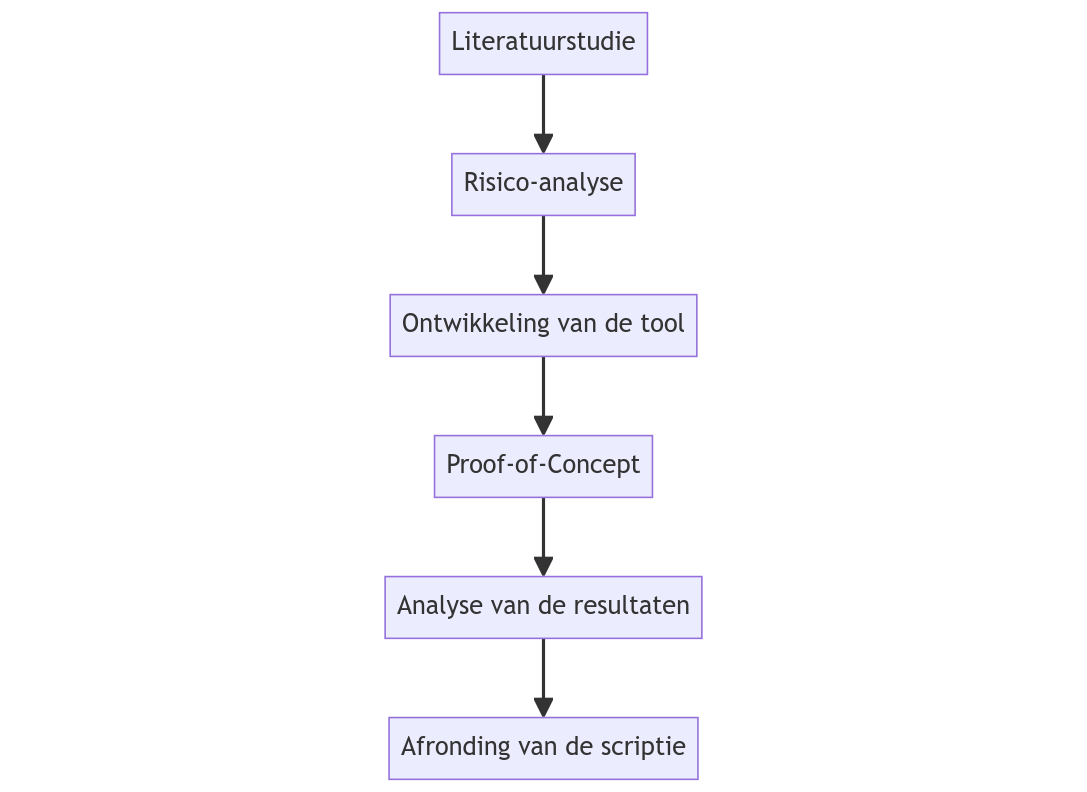
\includegraphics[width=.49\textwidth]
    {graphics/methodologie_flowchart.png}
    \caption{\label{fig:flowchart}Flowchart fasen methodologie}
\end{figure}


\subsection{Fase 1: Literatuurstudie}%
\label{sub:literatuurstudie}

De eerste fase omvat een grondige literatuurstudie die zich richt op het verzamelen van essenti\"ele configuratie en eigenschappen voor een grondig inventaris.
Daarnaast zullen ook bestaan\\de tools worden onderzocht die kunnen gebruikt worden bij het inventariseren van Linux-systemen.
Deze fase zal 2 weken in beslag nemen, en resulteert in een literatuurstudie die niet alleen de  eigenschappen van Linux-systemen identificeert die relevant zijn voor het inventaris, maar ook reeds bestaande tools die hiervoor gebruikt kunnen worden.

\subsection{Fase 2: Risico-analyse}%
\label{sub:risico_analyse}

De tweede fase richt zich op een risico-analyse, waarbij de ge\"identificeerde Linux-systeem\\eigenschappen binnen het inventaris kritisch worden ge\"evalueerd.
Via een diepgaande risico-\\analyse worden de impact van deze eigenschappen op het incidentresponseproces en hun bruikbaarheid beoordeeld.
Ook deze fase zal 2 weken in beslag nemen, en resulteert in een lijst van eigenschappen die een positieve bijdrage leveren aan het incidentresponseproces en een lijst van eigenschappen die een negatieve impact hebben.

\subsection{Fase 3: Ontwikkeling van de tool}%
\label{sub:ontwikkeling_van_de_tool}

De derde fase omvat de ontwikkeling van de tool, een Bash-script dat de eigenschappen van fase 2 gebruikt om een inventaris van het Linux-systeem op te stellen.
Het resultaat is een werkend Bash-script en zal ongeveer 3 weken in beslag nemen.

\subsection{Fase 4: Proof-of-Concept}%
\label{sub:proof_of_concept}

Na de ontwikkelingsfase volgt de Proof-of-\\Concept, waarbij een omgeving wordt opgezet met 5 Linux-servers met elk hun specifieke taak.
Deze fase zal ongeveer 1 week duren en omvat het testen van het script op de opgezette omgeving, resulterend in een inventaris van de omgeving.

\subsection{Fase 5: Analyse van de resultaten}%
\label{sub:analyse_van_de_resultaten}

Na het uitvoeren van het Proof-of-\\Concept worden de resultaten geanalyseerd.
Deze analyse vormt de basis voor de conclusie, waarbij de focus ligt op de kwaliteit en bruikbaarheid van het inventaris.
Beoordelingscriteria omvatten de volledigheid van het inventaris, de aanwezigheid van fouten en de impact op het incidentresponseproces.
Deze fase duurt 1 week.

\subsection{Fase 6: Afronding van de scriptie}%
\label{sub:afronding_van_de_scriptie}

De afsluitende fase richt zich op de voltooiing van de paper.
Ontbrekende hoofdstukken worden aangevuld, en de tekst wordt nauwkeurig nagelezen.
Het resultaat is een voltooide scriptie die voldoet aan alle vereiste normen en essenti\"ele hoofdstukken omvat.
Deze fase duurt 2 weken, maar er zal ook al aandacht aan worden besteed tijdens de voorgaande fasen.

%---------- Verwachte resultaten ----------------------------------------------
\section{Verwacht resultaat, conclusie}%
\label{sec:verwachte_resultaten}

De literatuurstudie heeft aangetoond welke systeemeigenschappen en configuratie we zouden kunnen gebruiken voor het opstellen van een inventaris.
De risico-analyse heeft kritieke eigenschappen van Linux-systemen ge\"identificeerd voor inventarisatie, waarbij een evenwicht is gezocht tussen positieve bijdragen aan het incident response proces en mogelijke negatieve effecten.

De ontwikkelde tool biedt een praktische oplossing voor het inventariseren van Linux-systemen te automatiseren.
Tijdens de Proof-of-Concept fase is aangetoond dat het script effectief is.
De inventarisatie was volledig en nauwkeurig, wat de potentie benadrukt om het incident response proces te versterken.


%%=============================================================================
%% Nmap
%%=============================================================================

\chapter{\IfLanguageName{dutch}{Uitvoer: Nmap-scan}{Output: Nmap-scan}}%
\label{ch:bijlage_nmap}

Deze bijlage bevat een voorbeeld van een Nmap-scan.
In deze demonstratie zal Nmap alle beschikbare poorten scannen, trachten het besturingssysteem en de actieve services te identificeren, en de versies van deze services te achterhalen.
De scan zal worden uitgevoerd op de \texttt{srv1} van de Proof of Concept, besproken in~\ref{ch:poc}.

Uit de uitvoer in~\ref{lst:bijlage-nmap-scan} kunnen we afleiden dat \texttt{srv1} een SSH-service draait op poort 22, een DNS-service op poort 53, en additionele services op poort 8053 en 9100.
Echter, bij de service op poort 9100 merken we op dat Nmap er niet in slaagt deze correct te identificeren en slechts een veronderstelling maakt omtrent de servicenaam.
Nmap heeft wel het besturingssysteem met succes gedetecteerd als Debian met Linux kernel versie 2.6.32, en heeft het correcte versies van andere ge\"identificeerde services gerapporteerd.

Merk wel op dat de fingerprint van de onbekende service werd weggelaten in de uitvoer van de scan, aangeduid met \texttt{[...]}.
Dit om de leesbaarheid van de uitvoer te verbeteren, aangezien de fingerprint van de onbekende service lang is.

\begin{longlisting}
  \begin{minted}[linenos,tabsize=4,breaklines]{console}
root@srv1:~# nmap -sS -sU -sV -A -p- localhost
Starting Nmap 7.93 ( https://nmap.org ) at 2024-05-09 10:51 UTC
Nmap scan report for localhost (127.0.0.1)
Host is up (0.000065s latency).
Other addresses for localhost (not scanned): ::1
Not shown: 65532 closed udp ports (port-unreach), 65530 closed tcp ports (reset)
PORT     STATE         SERVICE    VERSION
22/tcp   open          ssh        OpenSSH 9.2p1 Debian 2+deb12u2 (protocol 2.0)
| ssh-hostkey:
|   256 7823c0a999ef904f9f282137ef6f8c96 (ECDSA)
|_  256 3ad09088aa548a7bbaa6eb4fe41d88df (ED25519)
53/tcp   open          domain     ISC BIND 9.18.24-1 (Debian Linux)
953/tcp  open          rndc?
8053/tcp open          senomix02?
| fingerprint-strings:
|   FourOhFourRequest:
|     HTTP/1.0 404 No such URL
|     Connection: close
|     Content-Type: text/plain
|     Date: Thu, 09 May 2024 10:51:17 GMT
|     Expires: Thu, 09 May 2024 10:51:17 GMT
|     Last-Modified: Thu, 09 May 2024 10:51:17 GMT
|     Pragma: no-cache
|     Cache-Control: no-cache
|     Server: libisc
|     Content-Length: 14
|     such URL.
|   GetRequest:
|     HTTP/1.0 200 OK
|     Connection: close
|     Content-Type: text/xml
|     Date: Thu, 09 May 2024 10:51:17 GMT
|     Expires: Thu, 09 May 2024 10:51:17 GMT
|     Last-Modified: Thu, 09 May 2024 10:51:17 GMT
|     Pragma: no-cache
|     Cache-Control: no-cache
|     Server: libisc
|     Content-Length: 55113
|     <?xml version="1.0" encoding="UTF-8"?>
|     <?xml-stylesheet type="text/xsl" href="/bind9.xsl"?>
|_    <statistics version="3.13"><server><boot-time>2024-05-09T10:45:33.614Z</boot-time><config-time>2024-05-09T10:45:41.610Z</config-time><current-time>2024-05-09T10:51:17.111Z</current-time><version>9.18.24-1-Debian</version><counters type="opcode"><counter name="QUERY">25</counter><counter name="IQUERY">0</counter><counter name="STATUS">1</counter><counter name="RESERVED3">0</counter><counter name="NOTIFY">0</counter><counter name="UPDATE">0</counter><counter name="RESERVED6">0</counter><counter name="RESERVED7">0</counter><counter name="
9100/tcp open          jetdirect?
53/udp   open          domain     ISC BIND 9.18.24-1 (Debian Linux)
|_dns-recursion: Recursion appears to be enabled
| dns-nsid:
|_  bind.version: 9.18.24-1-Debian
68/udp   open|filtered dhcpc
323/udp  open|filtered unknown
1 service unrecognized despite returning data. If you know the service/version, please submit the following fingerprint at https://nmap.org/cgi-bin/submit.cgi?new-service :
[...]
Device type: general purpose
Running: Linux 2.6.X
OS CPE: cpe:/o:linux:linux_kernel:2.6.32
OS details: Linux 2.6.32
Network Distance: 0 hops
Service Info: OS: Linux; CPE: cpe:/o:linux:linux_kernel

OS and Service detection performed. Please report any incorrect results at https://nmap.org/submit/ .
Nmap done: 1 IP address (1 host up) scanned in 131.26 seconds
  \end{minted}
  \caption{Een grondige scan van \texttt{srv1}, waar Nmap alle poorten zal scannen, het besturingssysteem en de services zal proberen te detecteren en de versies van de services zal proberen te achterhalen.}
  \label{lst:bijlage-nmap-scan}
\end{longlisting}

%%=============================================================================
%% Puppetboard
%%=============================================================================

\chapter{\IfLanguageName{dutch}{Puppetboard}{Puppetboard}}%
\label{ch:bijlage_puppetboard}

Afbeelding~\ref{fig:puppetboard-home} toont een voorbeeld van de startpagina van Puppetboard.
Hier krijgen we een beknopt overzicht van het aantal nodes dat door Puppet wordt beheerd en de totale hoeveelheid resources die wordt beheerd.
Ook kunnen we zien hoeveel runs zijn mislukt en hoeveel succesvol waren.
Onder de grafieken bevindt zich een lijst van servers waarop Puppet recentelijk een run heeft uitgevoerd om de gedefinieerde configuratie toe te passen.

\begin{figure}[h!]
    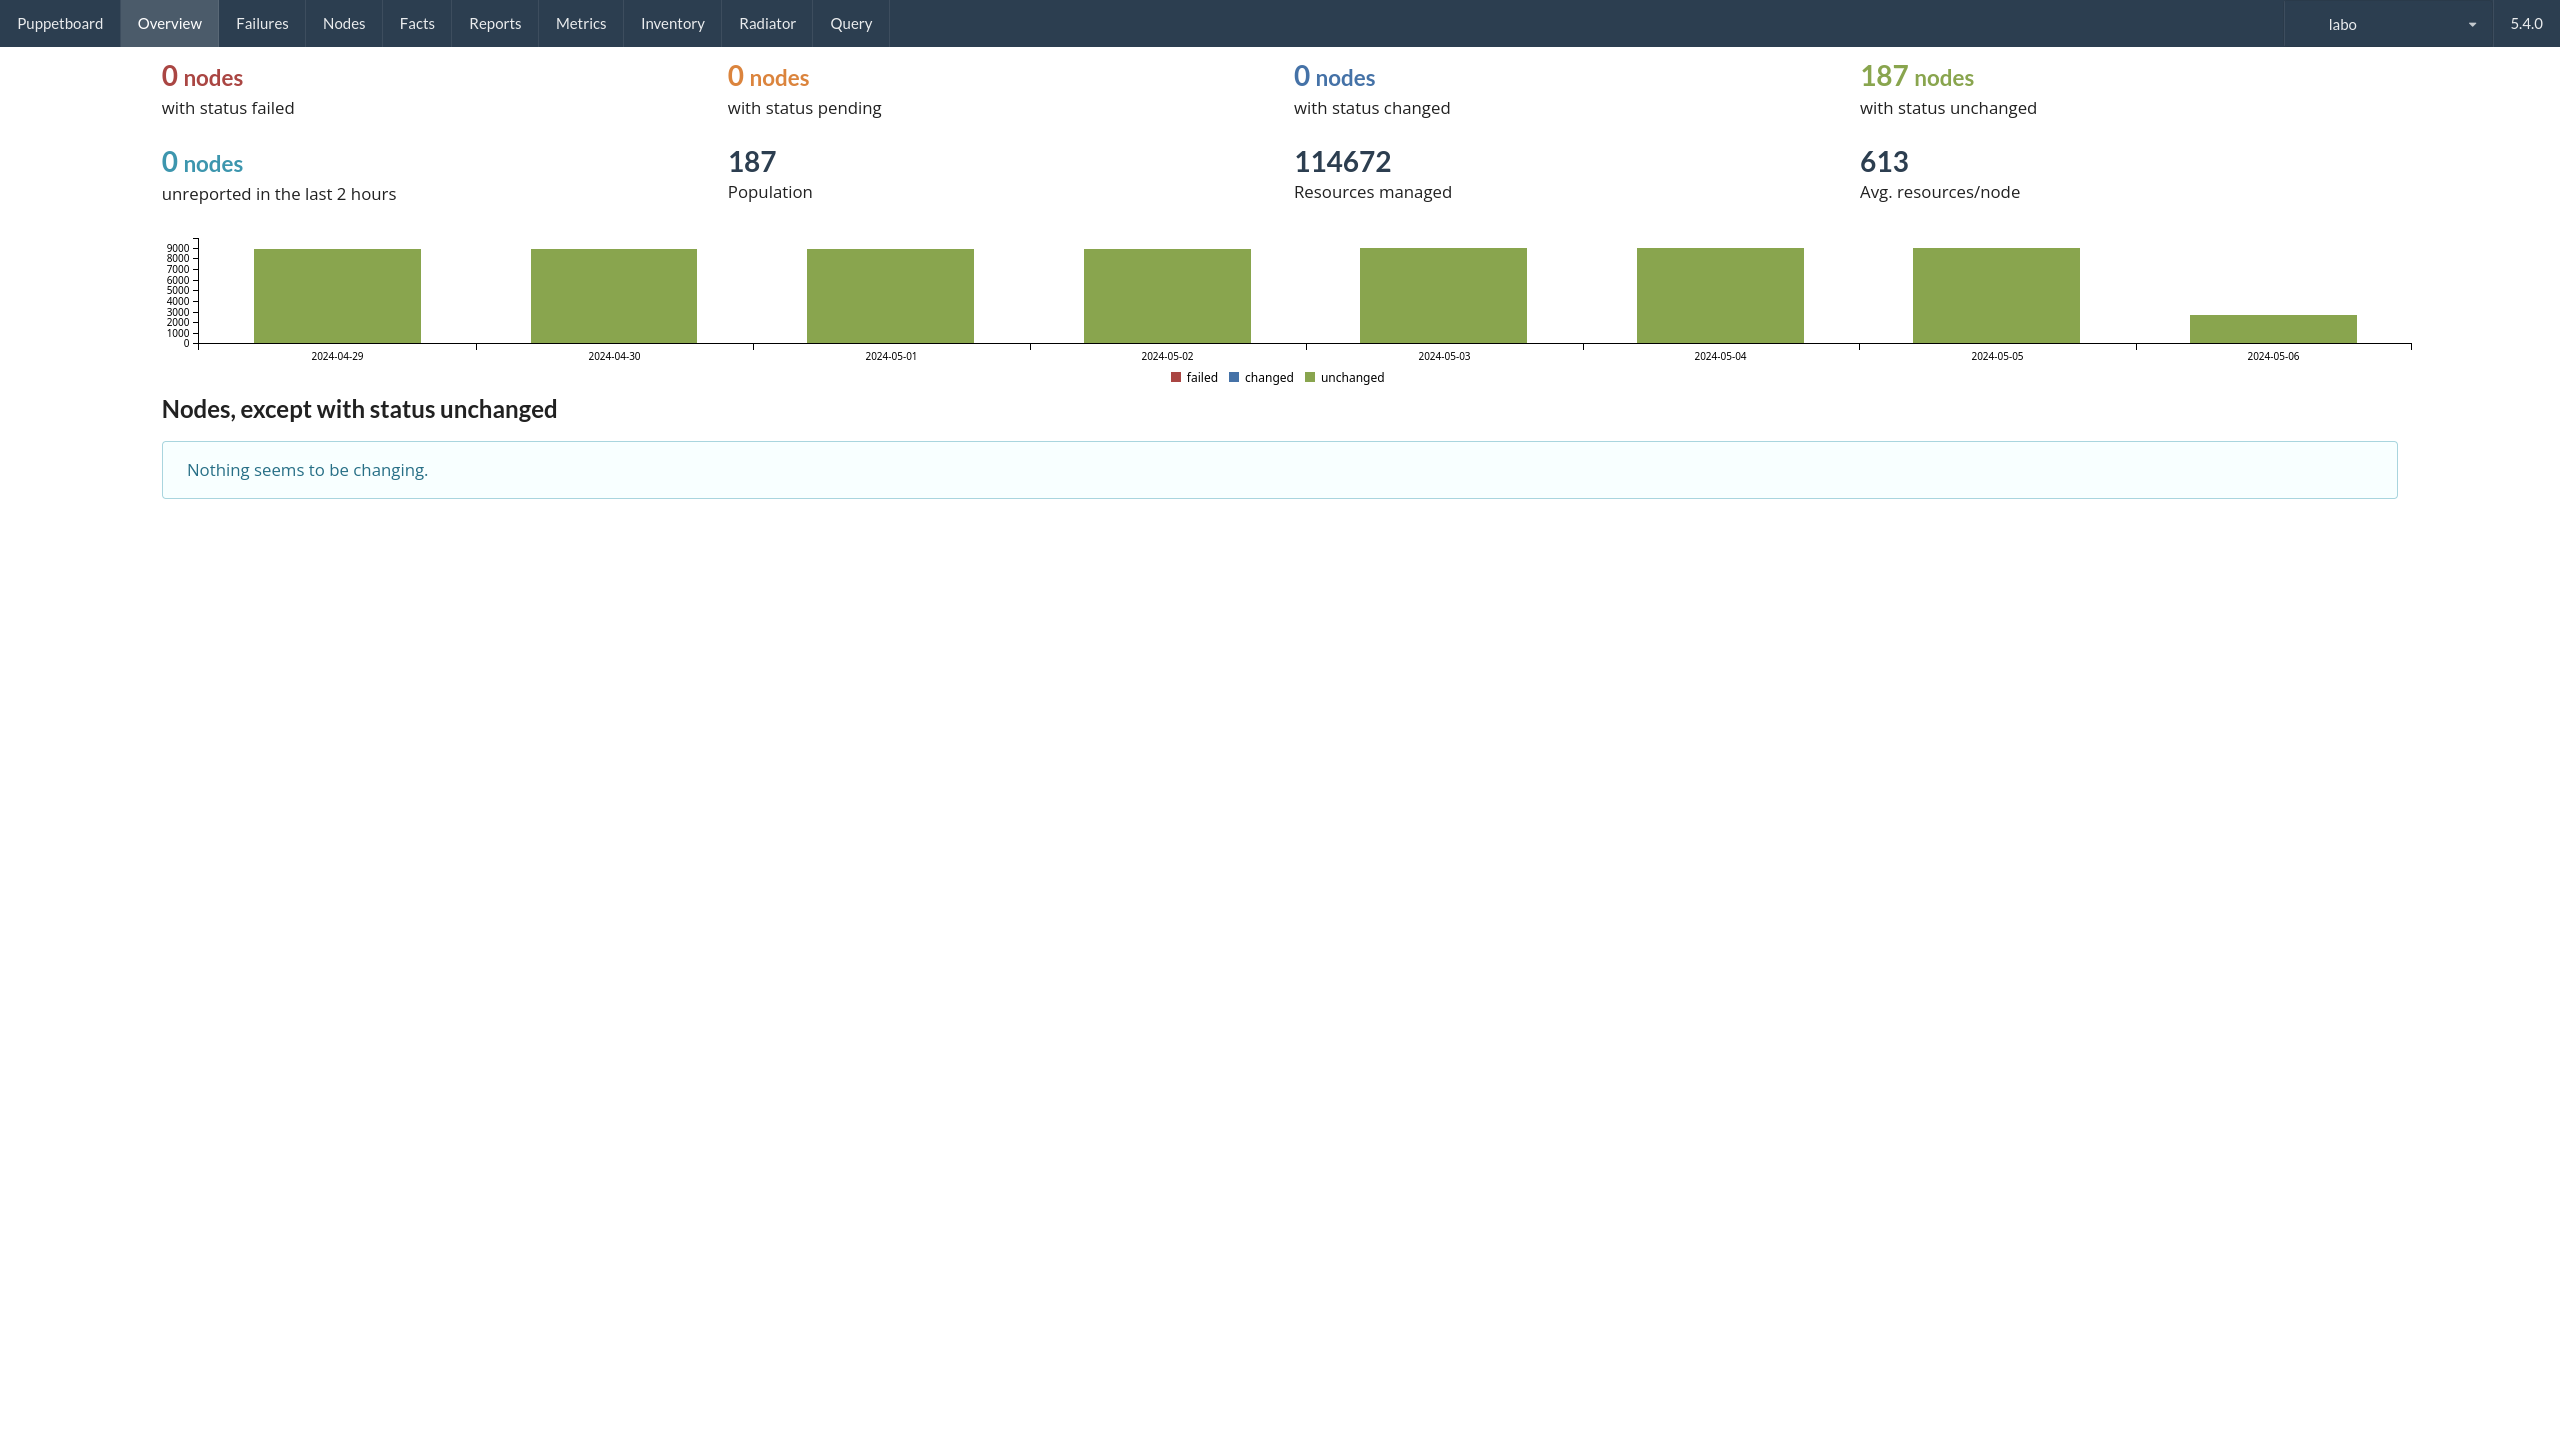
\includegraphics[width=\textwidth]
    {./graphics/state-of-the-art/puppetboard/puppetboard-home.png}
    \caption[Puppetboard startpagina.]{\label{fig:puppetboard-home}Voorbeeld van de Puppetboard startpagina.}
\end{figure}

Afbeelding~\ref{fig:puppetboard-inventory} toont een overzicht van alle nodes die door Puppet worden beheerd.
Alsook wanneer de laatste run was en of deze succesvol was.

\begin{figure}[h!]
    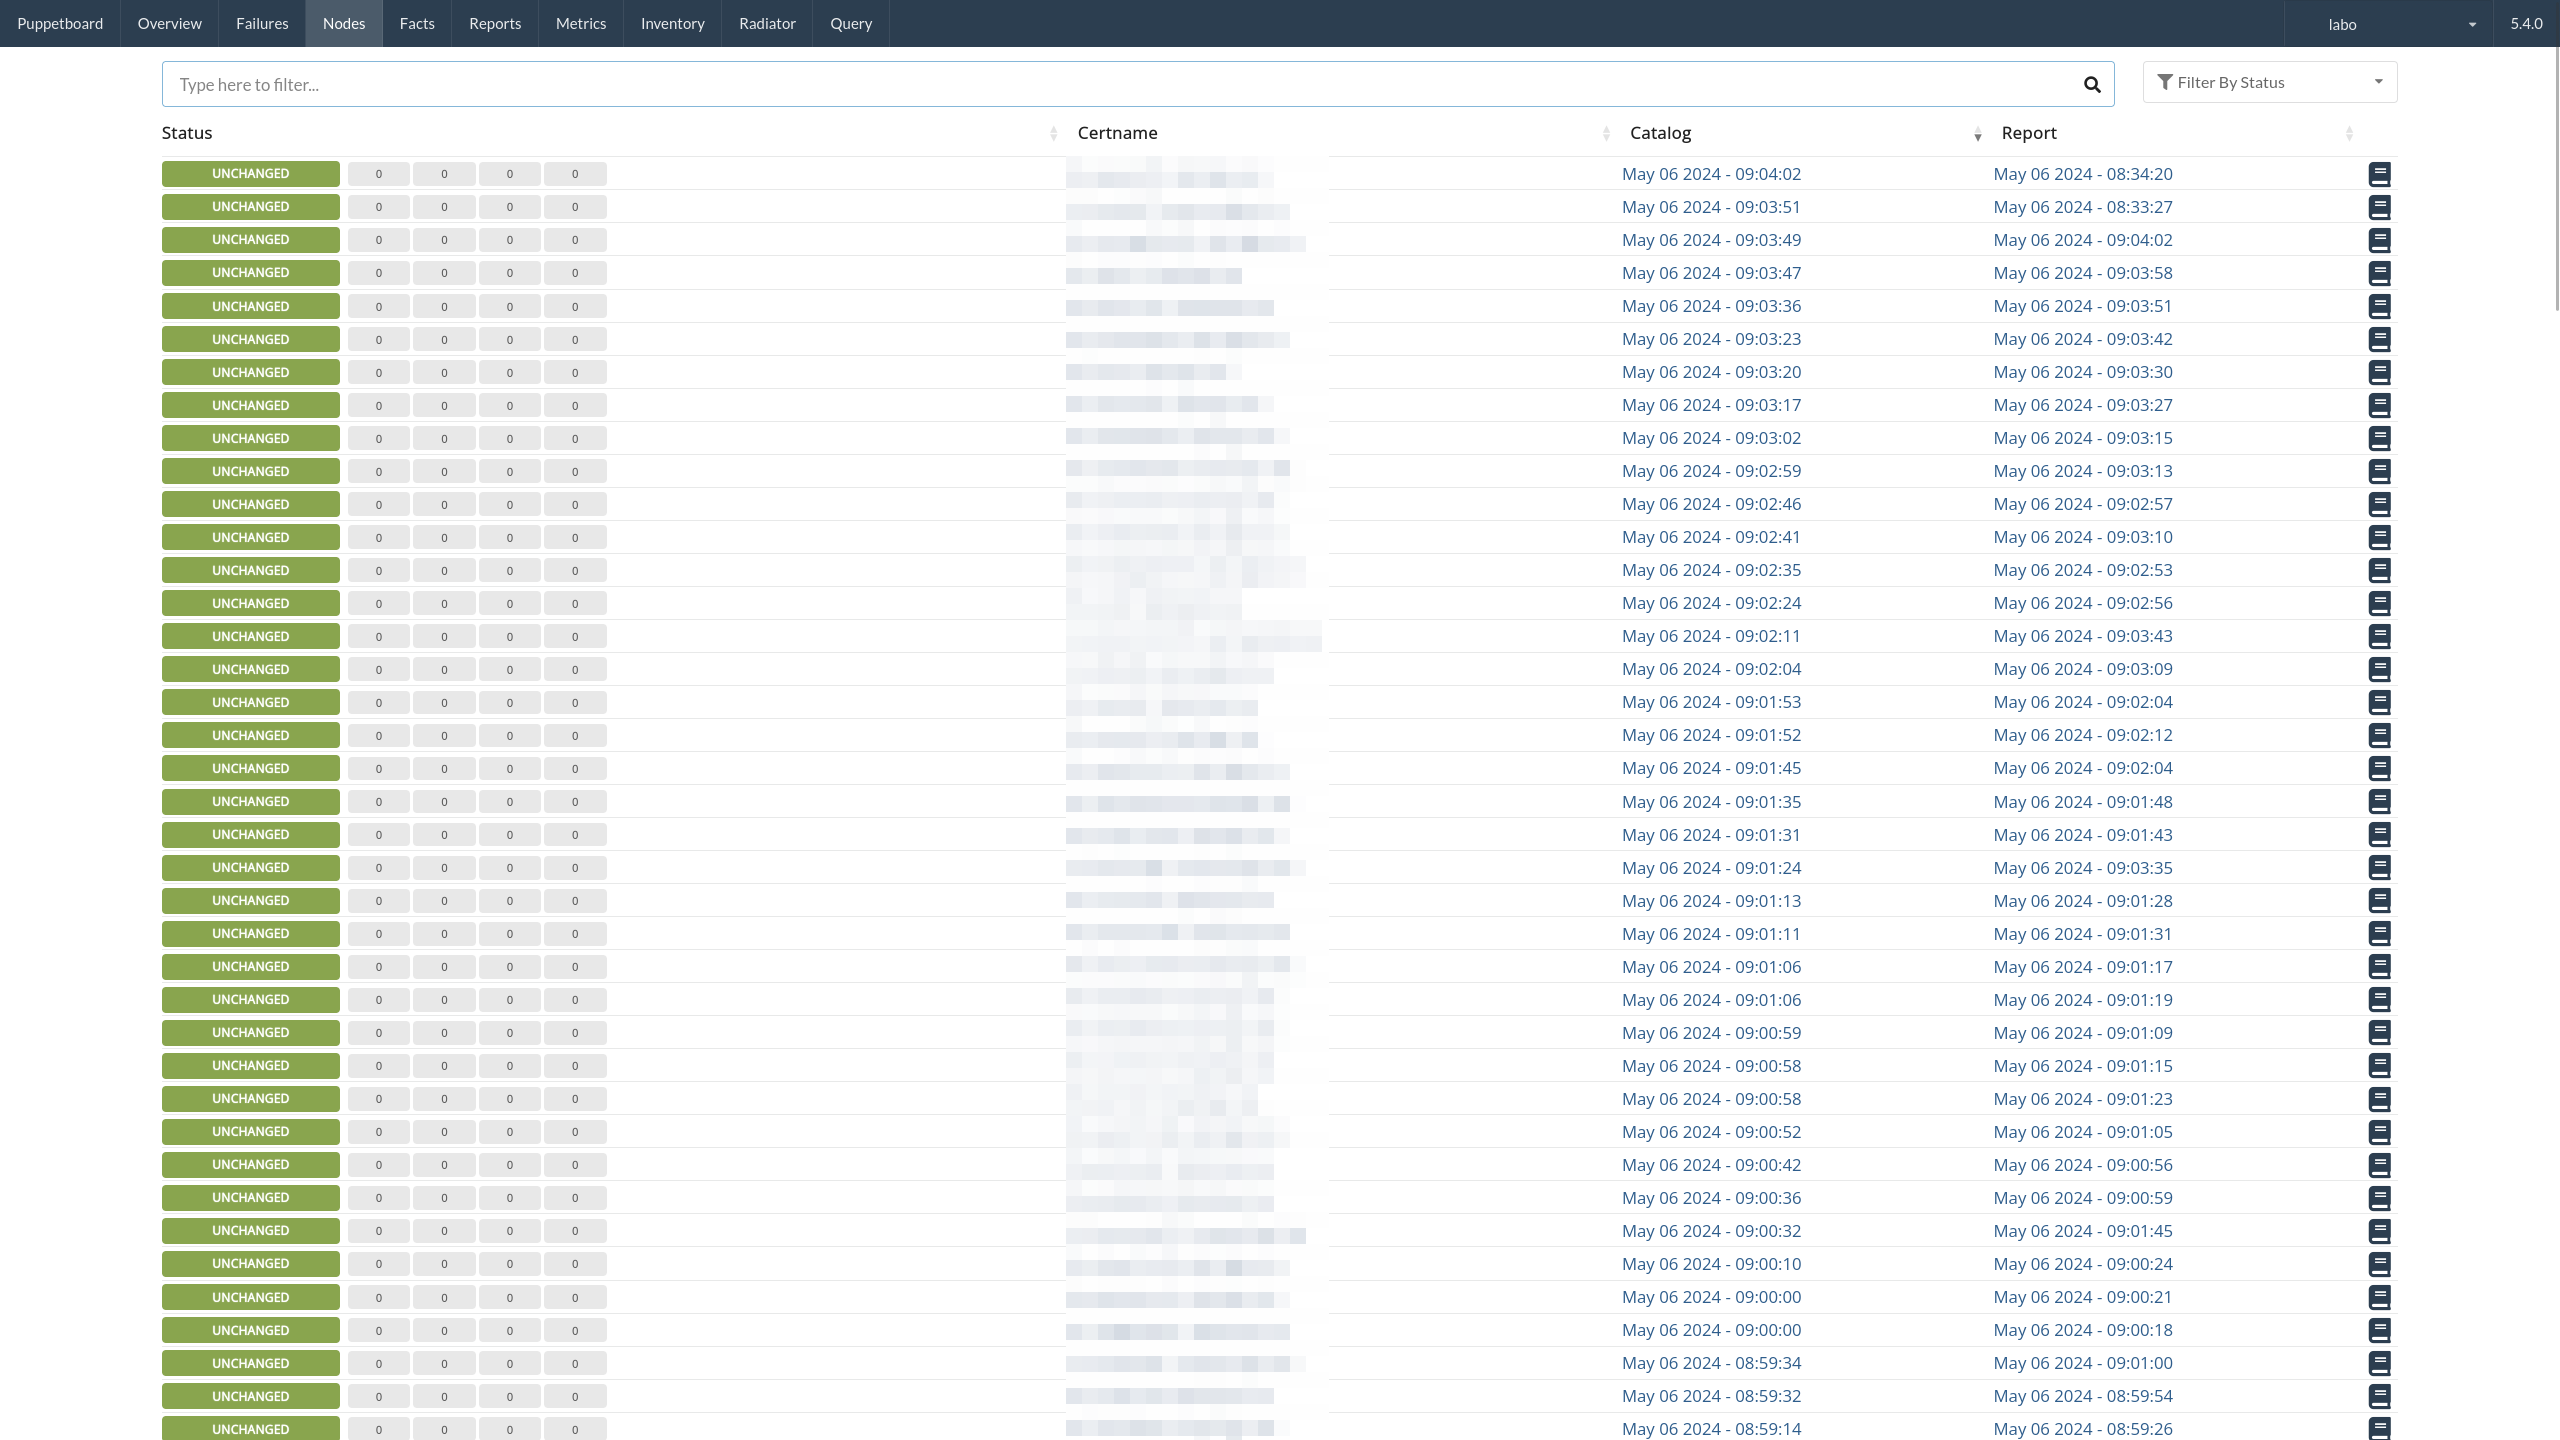
\includegraphics[width=\textwidth]
    {./graphics/state-of-the-art/puppetboard/puppetboard-hosts.png}
    \caption[Puppetboard inventaris van nodes.]{\label{fig:puppetboard-inventory}Voorbeeld van de Puppetboard waar we alle nodes van het inventaris kunnen zien.}
\end{figure}

Afbeelding~\ref{fig:puppetboard-example-4} toont een lijst van verschillende nodes die door Puppet worden beheerd.
Men kan de hostname, IP-adres, besturingssysteem, CPU-arhitectuur, kernelversie en de Puppet-agent versie zien.

\begin{figure}[h!]
    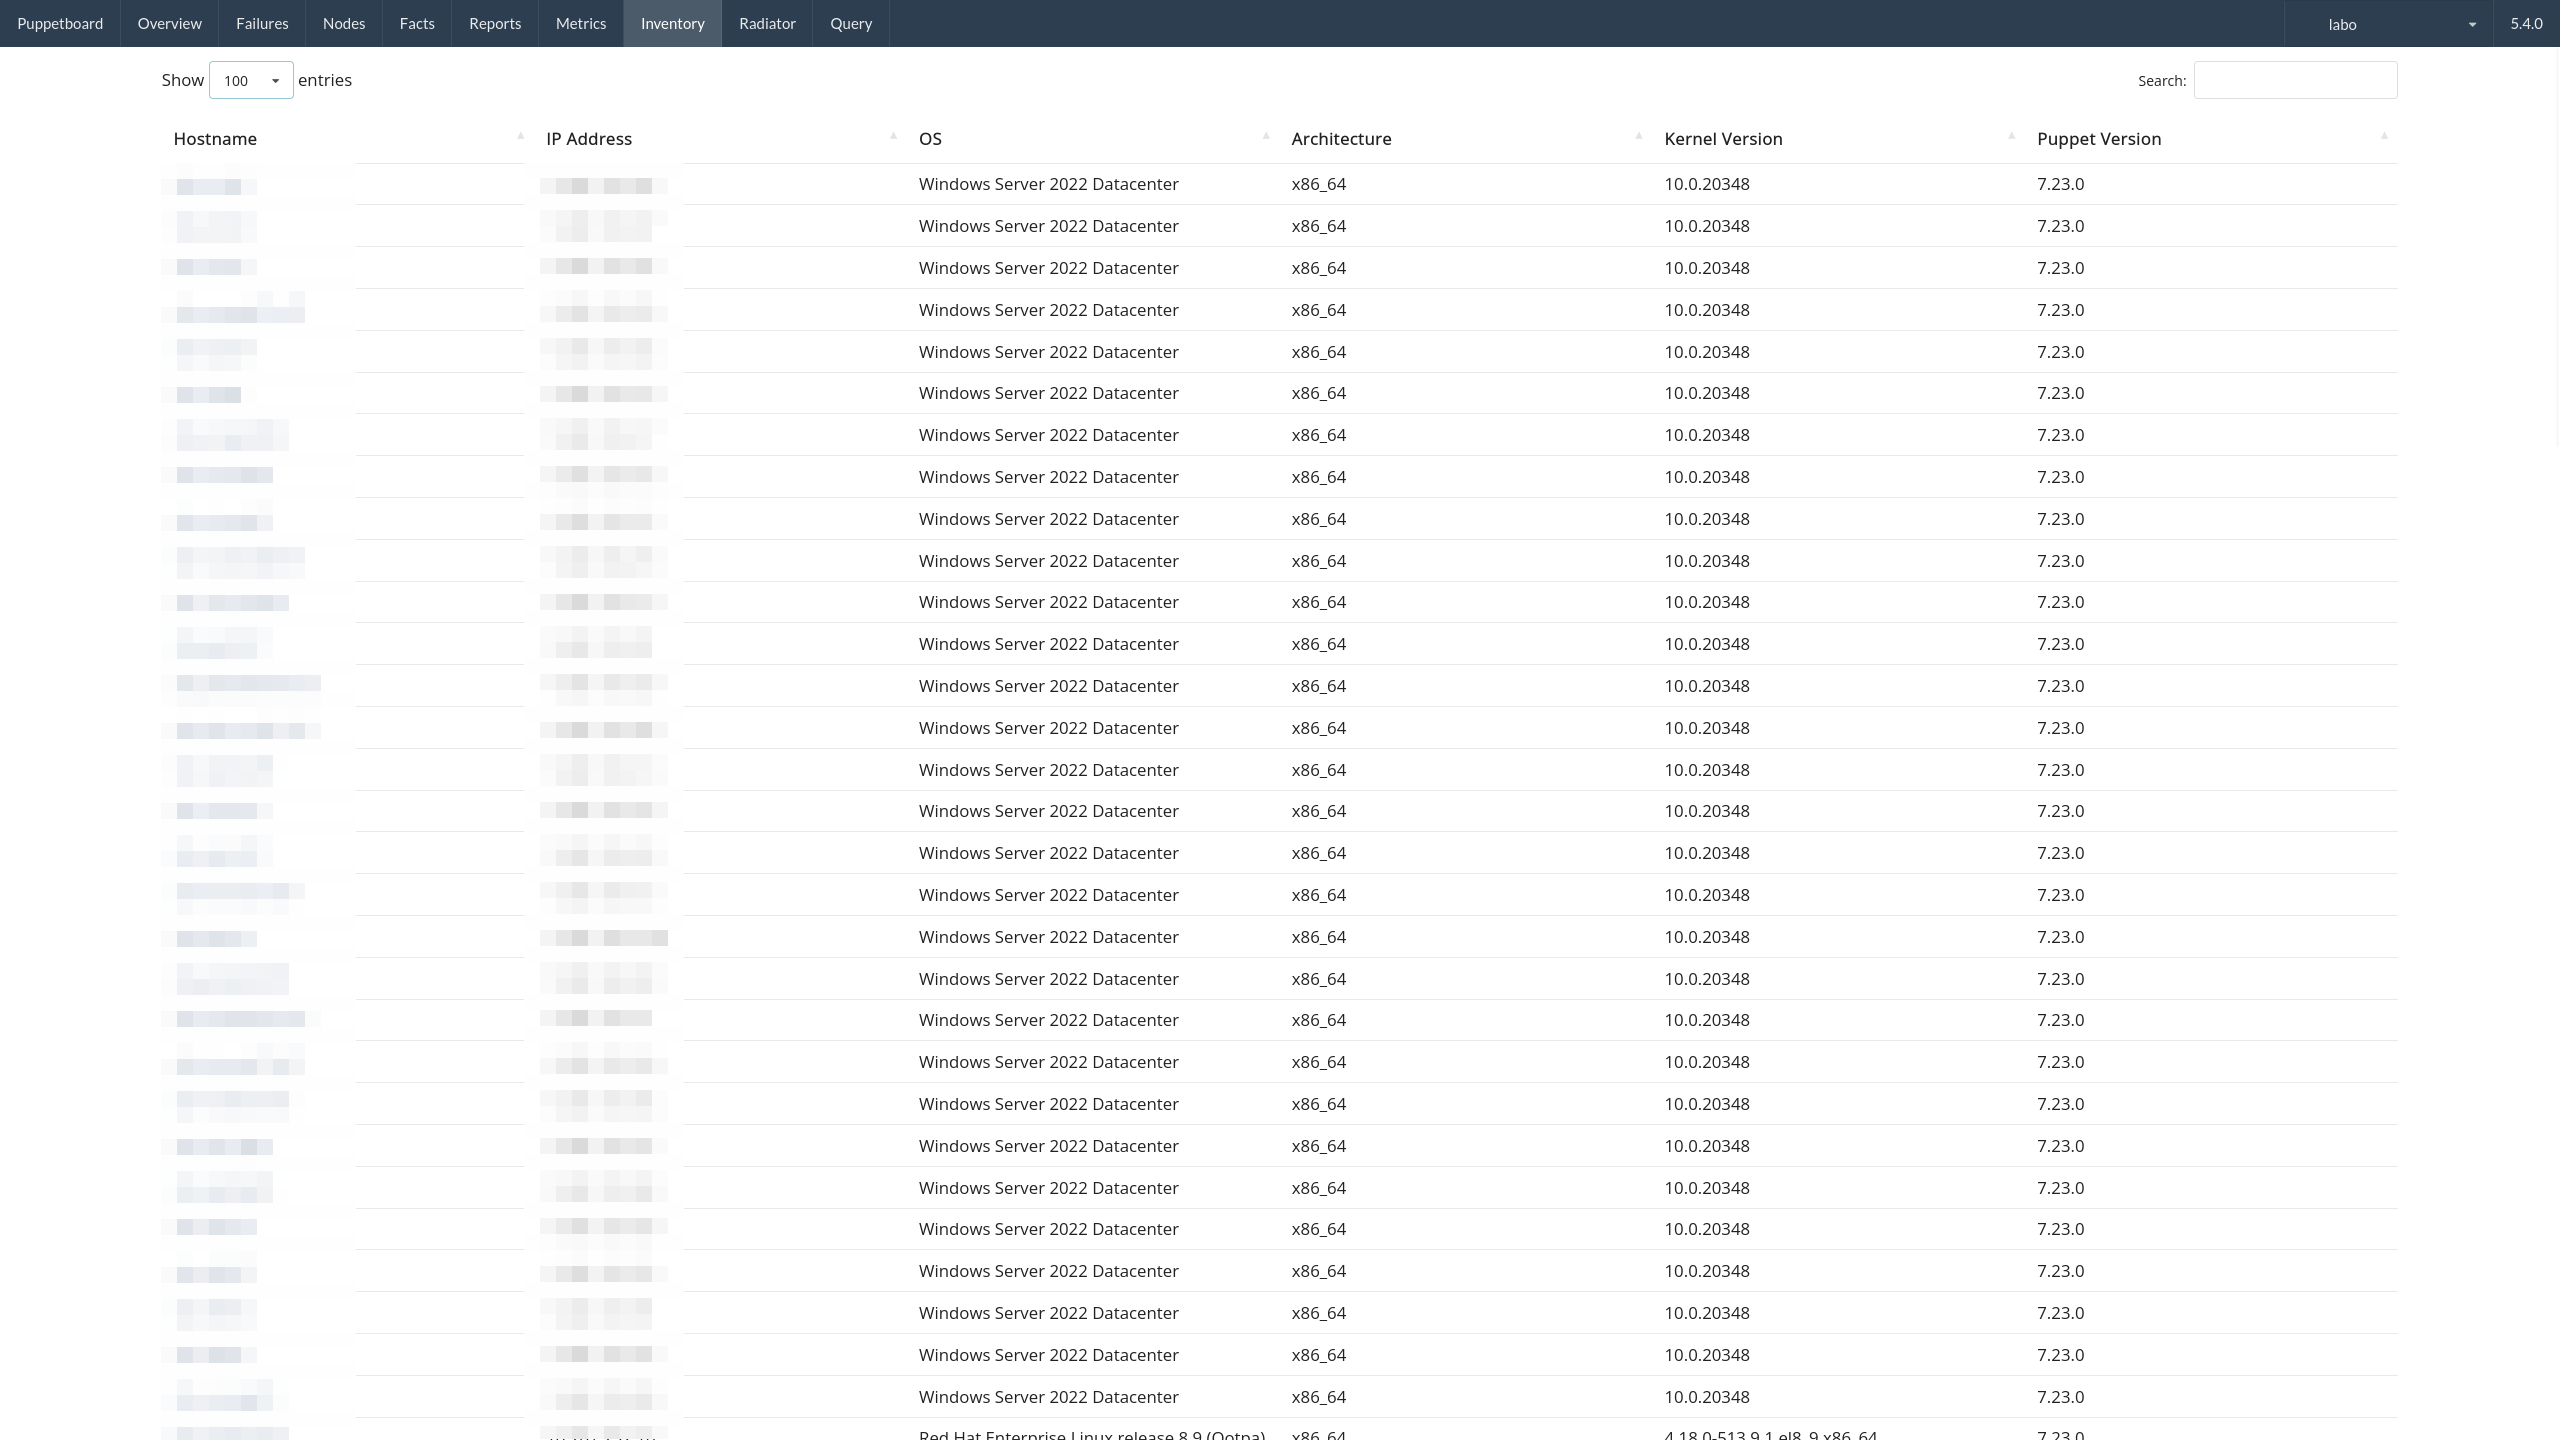
\includegraphics[width=\textwidth]
    {./graphics/state-of-the-art/puppetboard/puppetboard-inventory.png}
    \caption[Basisinformatie op Puppetboard.]{\label{fig:puppetboard-example-4}Voorbeeld van de Puppetboard waar we basis informatie over het systeem kunnen vinden.}
\end{figure}

%%=============================================================================
%% Red Hat Satellite
%%=============================================================================

\chapter{\IfLanguageName{dutch}{Red Hat Satellite}{Red Hat Satellite}}%
\label{ch:bijlage_red_hat_satellite}

Schermafbeelding~\ref{fig:rhel-sat-hosts} toont de pagina waarop enkele hosts worden weergegeven die geregistreerd zijn in Red Hat Satellite.
Voor elke host worden details getoond, zoals de hostname, het besturingssysteem, het model en de eigenaar van de host.
Door te klikken op een specifieke host, krijgen we een overzicht te zien van die host, zoals te zien is in schermafbeelding~\ref{fig:rhel-sat-host-overview}.
Hier worden meer gegevens over de host weergegeven, waaronder de status, toegekende IP-adressen en het MAC-adres.
Ook wordt informatie getoond over de ``Errata'' die van toepassing zijn op deze host, wat updates zijn die nog niet zijn ge\"installeerd, waaronder verbeteringen, beveiligingsupdates of bugfixes.

\begin{figure}[h!]
    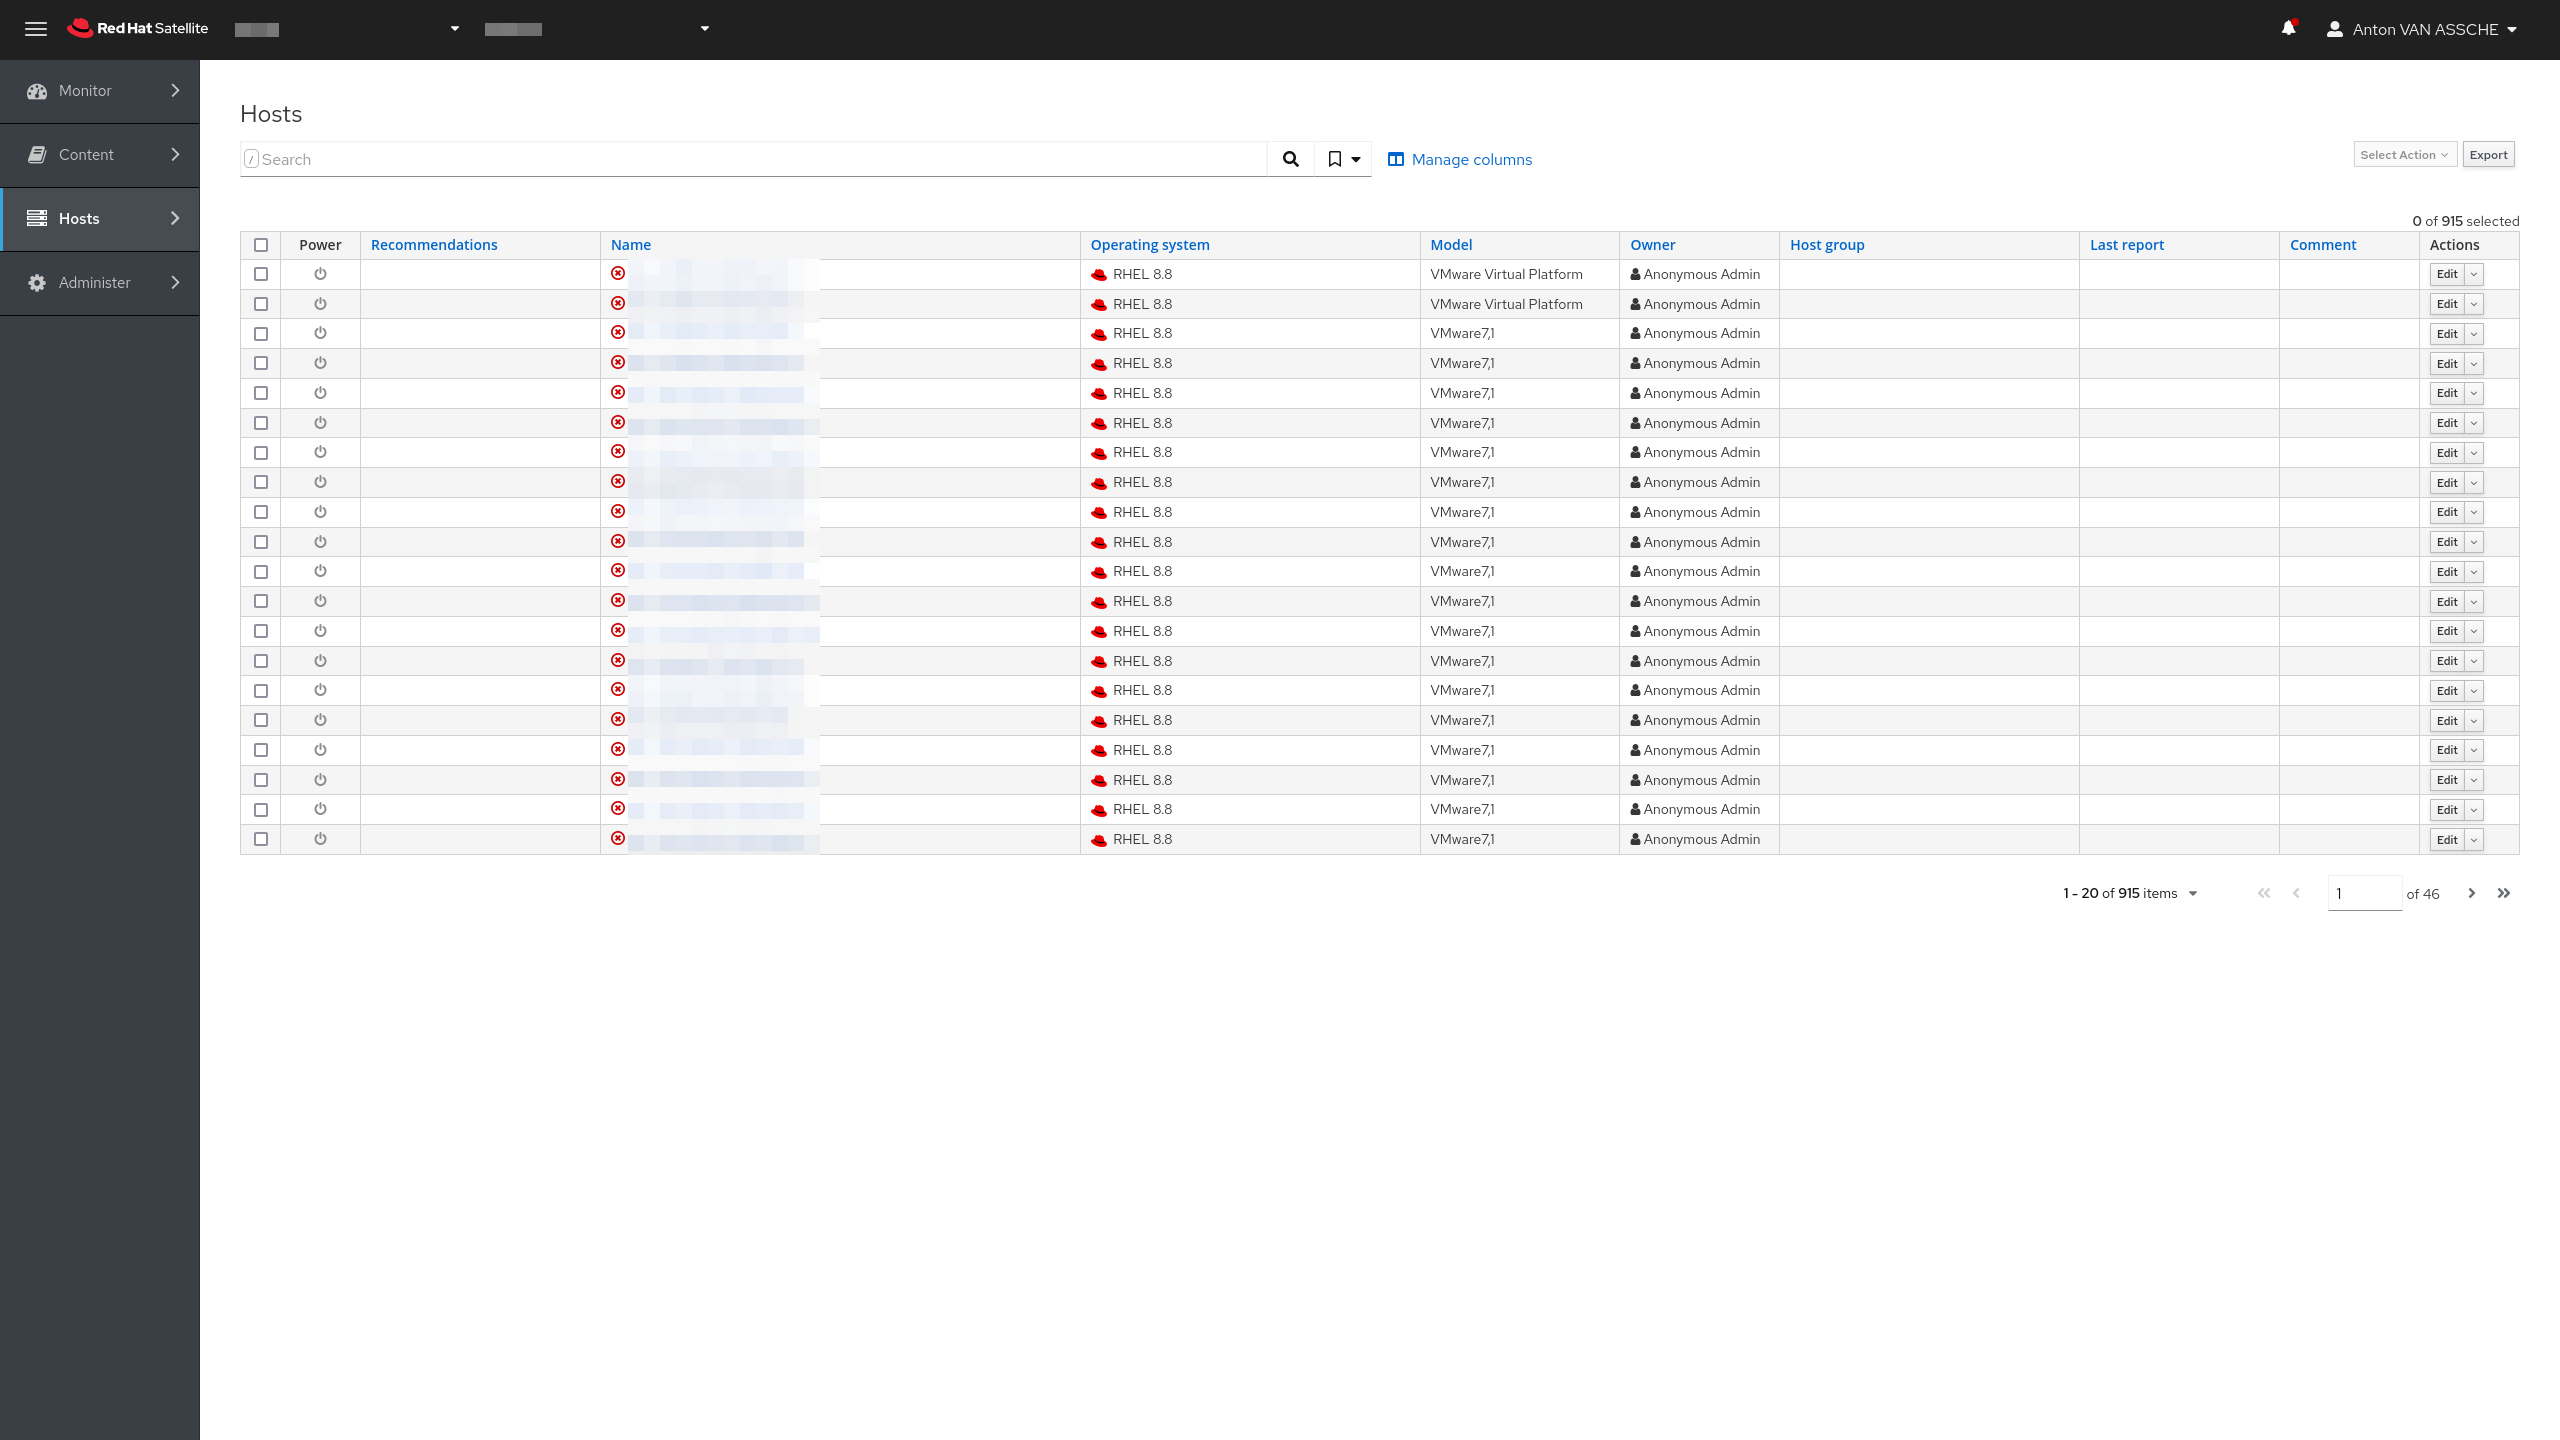
\includegraphics[width=\textwidth]
    {./graphics/state-of-the-art/rhel-satellite/rhel-sat-hosts.png}
    \caption{\label{fig:rhel-sat-hosts}Lijst van hosts die geregistreerd zijn in Red Hat Satellite.}
\end{figure}

\begin{figure}[h!]
    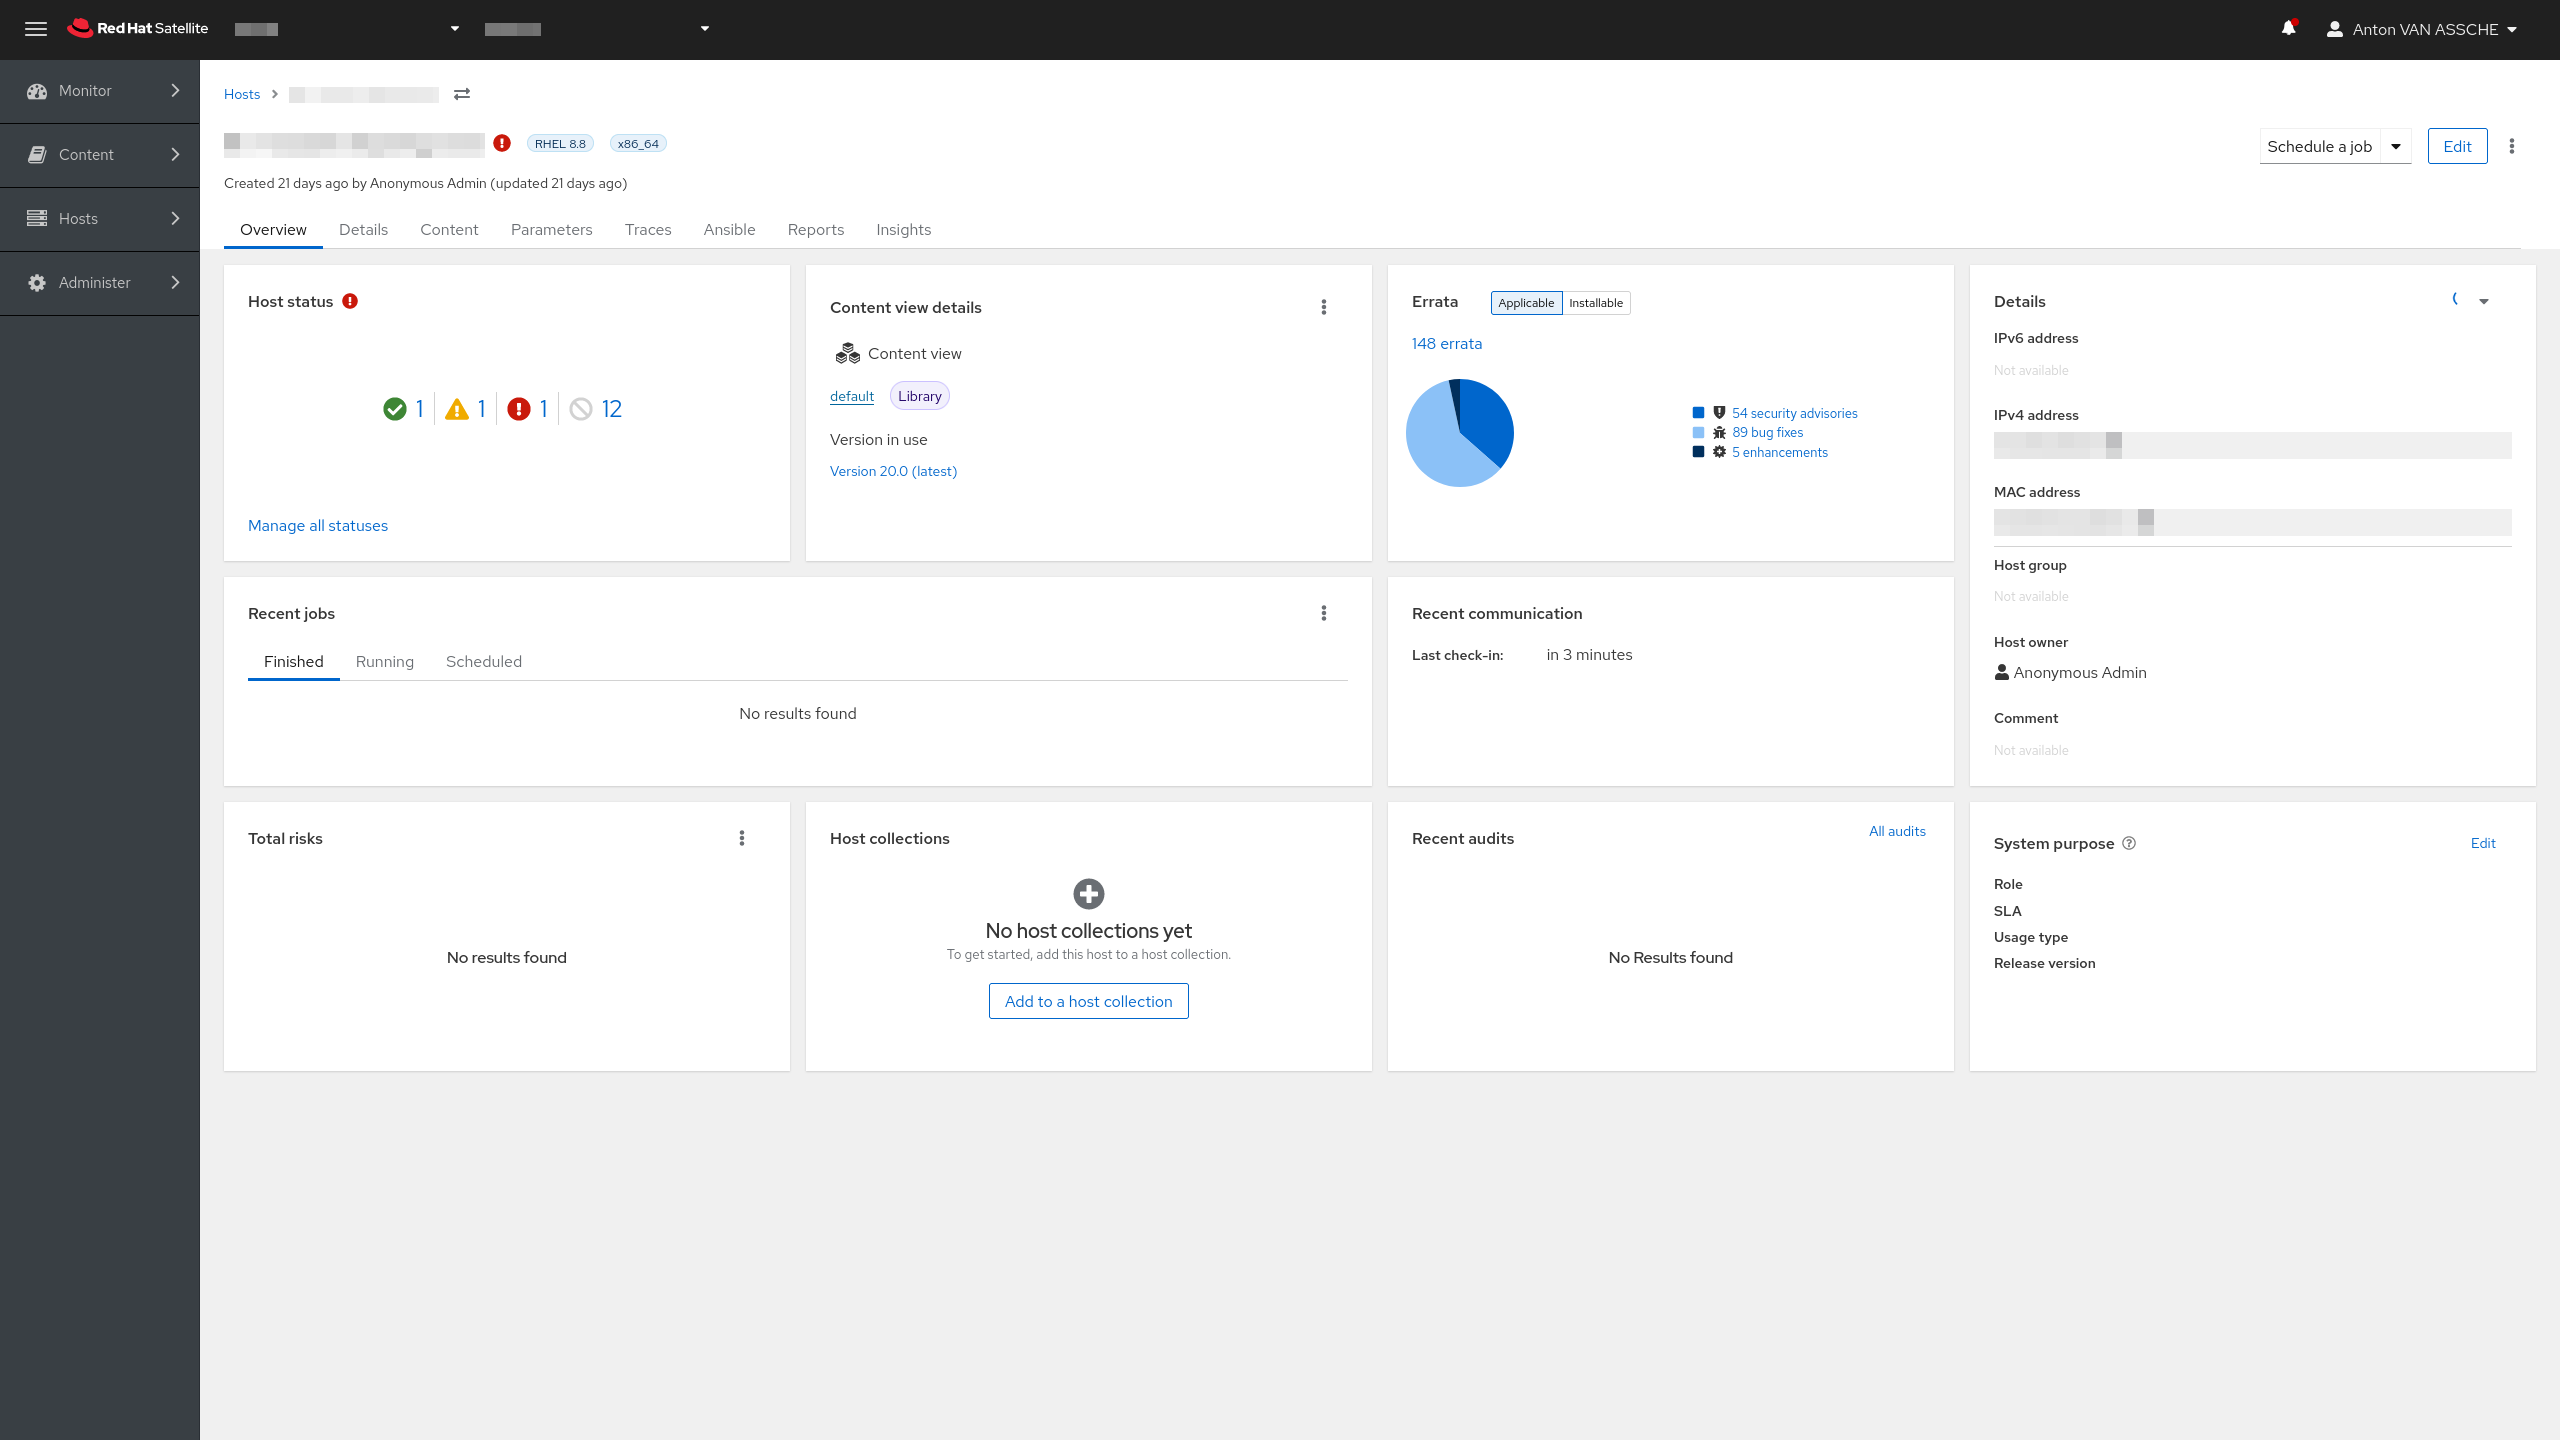
\includegraphics[width=\textwidth]
    {./graphics/state-of-the-art/rhel-satellite/rhel-sat-host-overview.png}
    \caption{\label{fig:rhel-sat-host-overview}Algemeen overzicht van een host in Red Hat Satellite.}
\end{figure}

Door te navigeren naar het tabblad ``Details'' krijgen we een uitgebreider overzicht van de host te zien, zoals weergegeven in schermafbeelding~\ref{fig:rhel-sat-host-details}.
Hier worden veel meer gegevens over de host verstrekt, zoals het besturingssysteem, de kernelversie, de architectuur, informatie over geheugen en CPU en de netwerkinterfaces.
Vervolgens kunnen we doorklikken naar het tabblad ``Content'' en vervolgens naar ``Packages'', waar we een lijst krijgen van alle ge\"installeerde pakketten op de host, zoals weergegeven in schermafbeelding~\ref{fig:rhel-sat-host-pkgs}.
Klikken op een specifiek pakket geeft ons meer informatie over dat pakket, zoals de versie, de release, de grootte en de datum van installatie, deze informatie is echter niet zichtbaar in de schermafbeelding.

\begin{figure}[h!]
    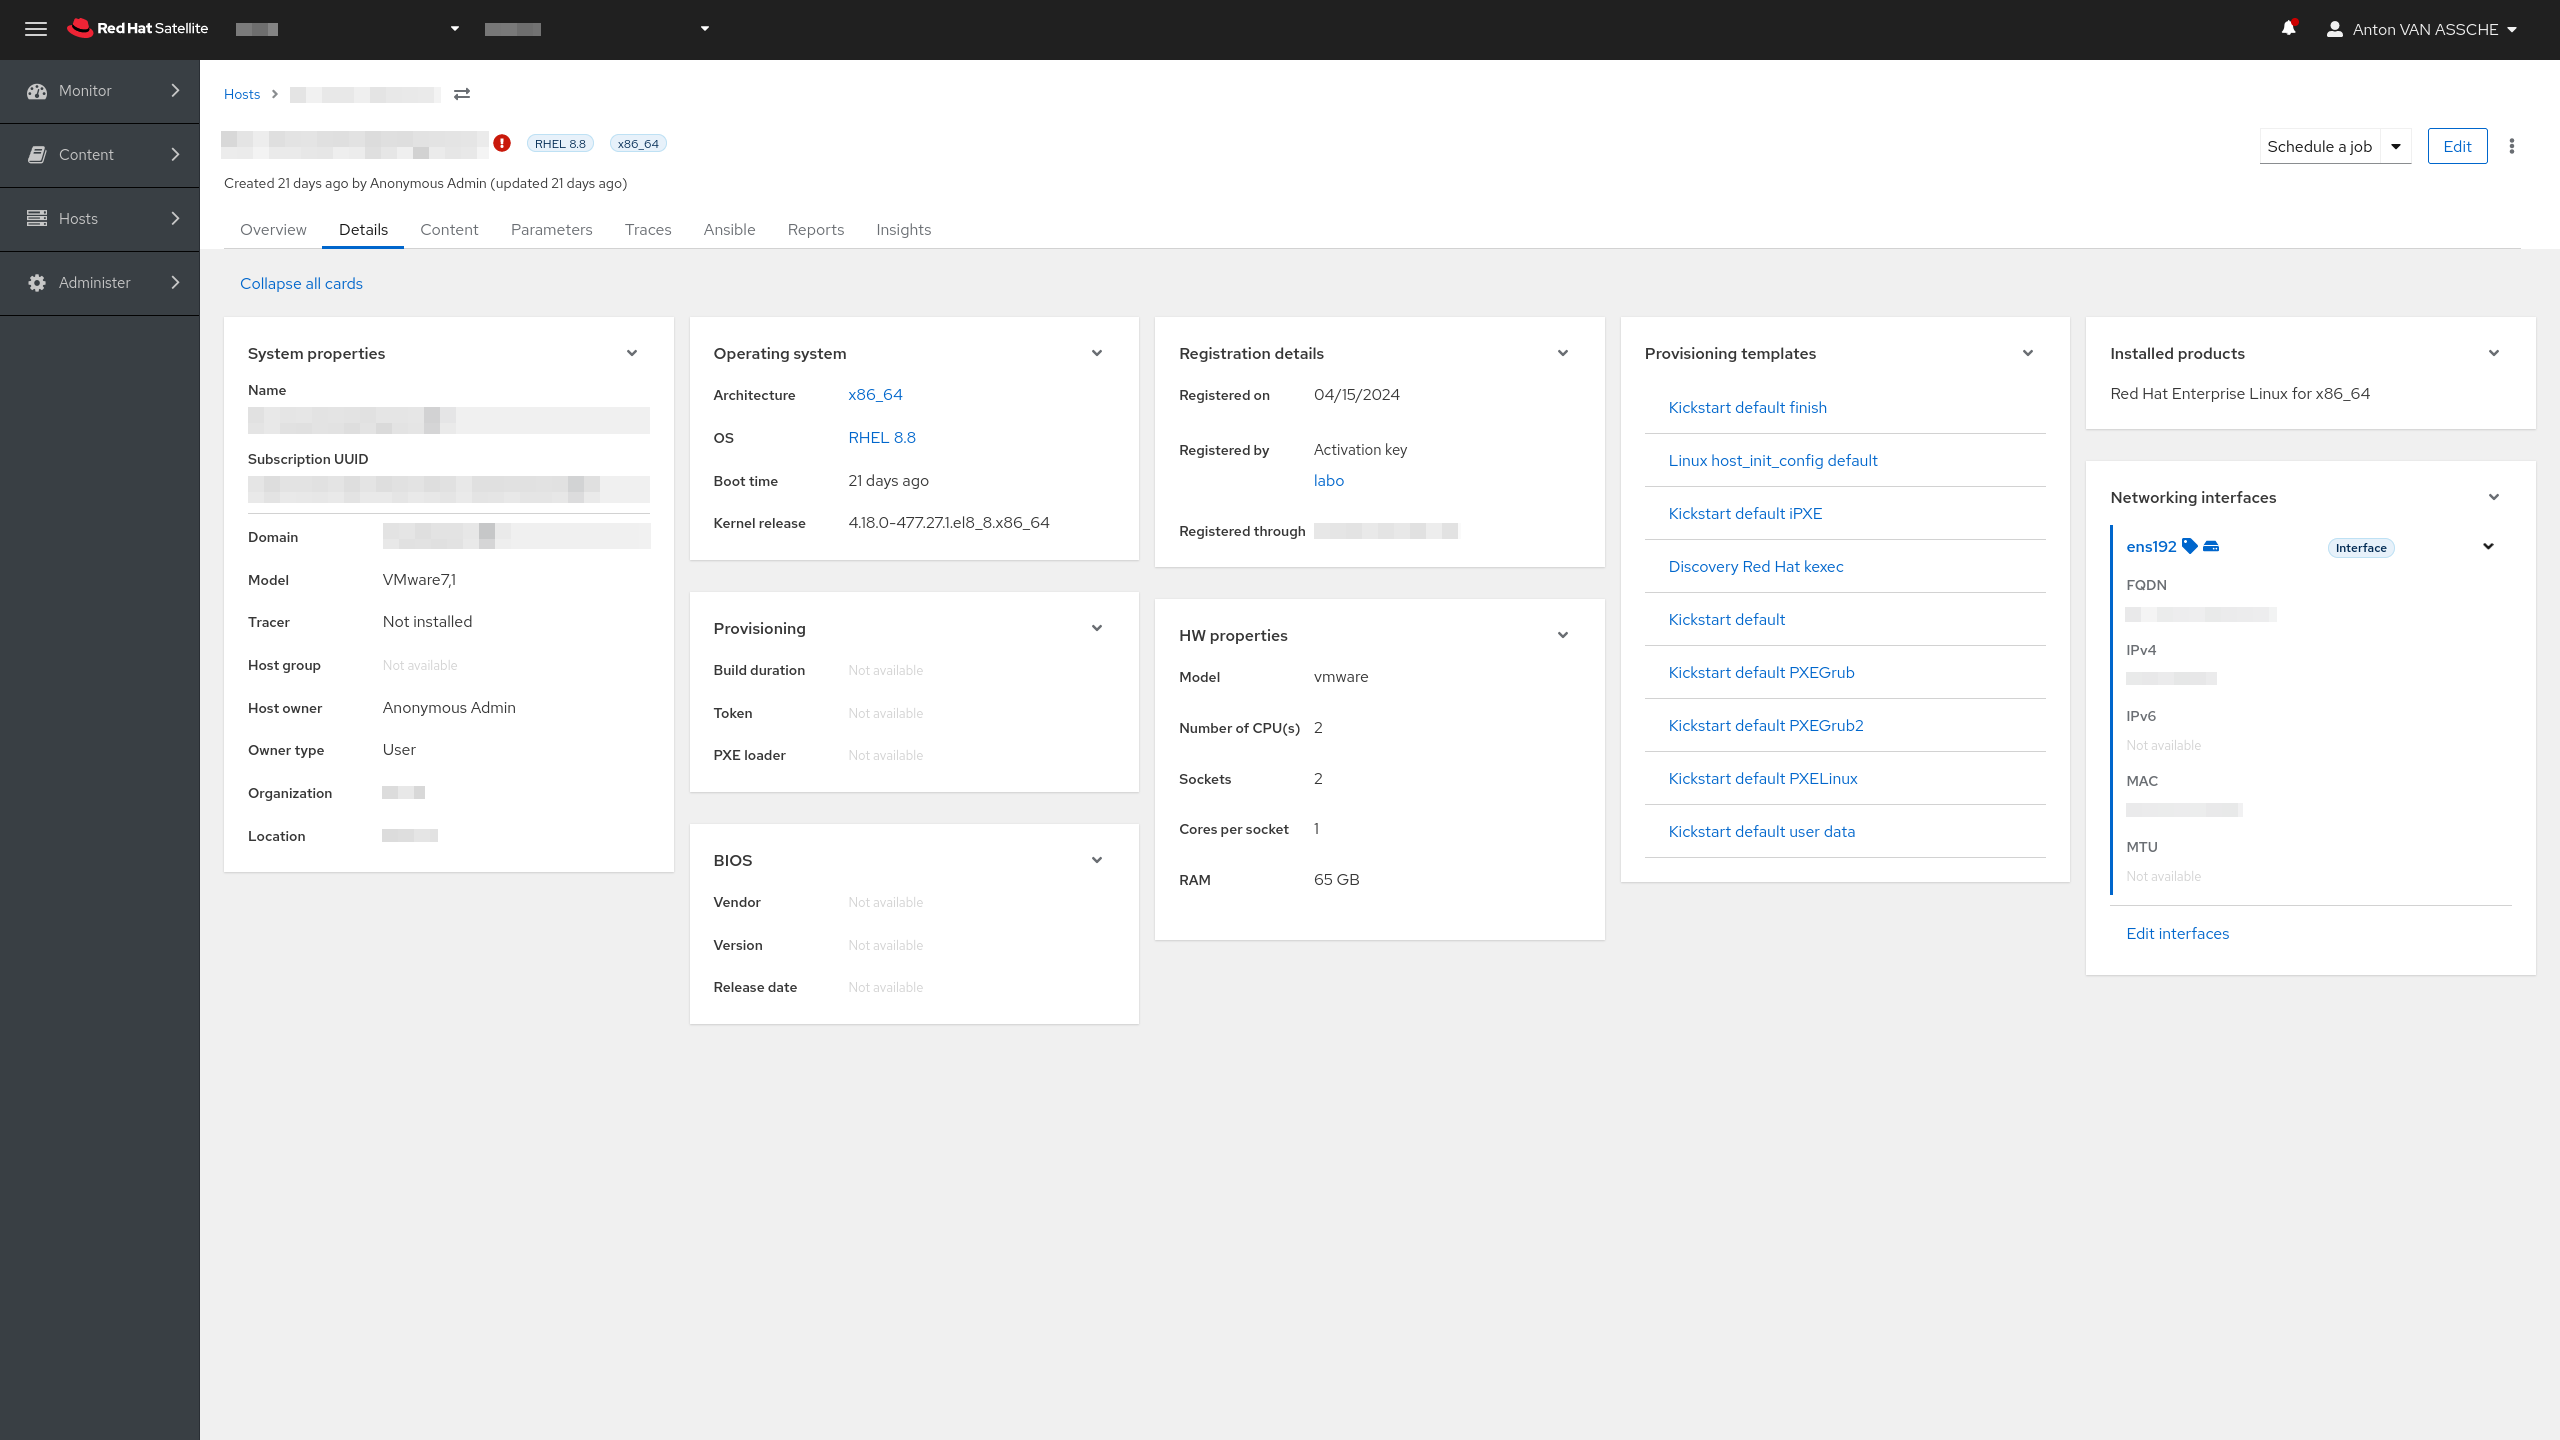
\includegraphics[width=\textwidth]
    {./graphics/state-of-the-art/rhel-satellite/rhel-sat-host-details.png}
    \caption{\label{fig:rhel-sat-host-details}Details van een host in Red Hat Satellite.}
\end{figure}

\begin{figure}[h!]
    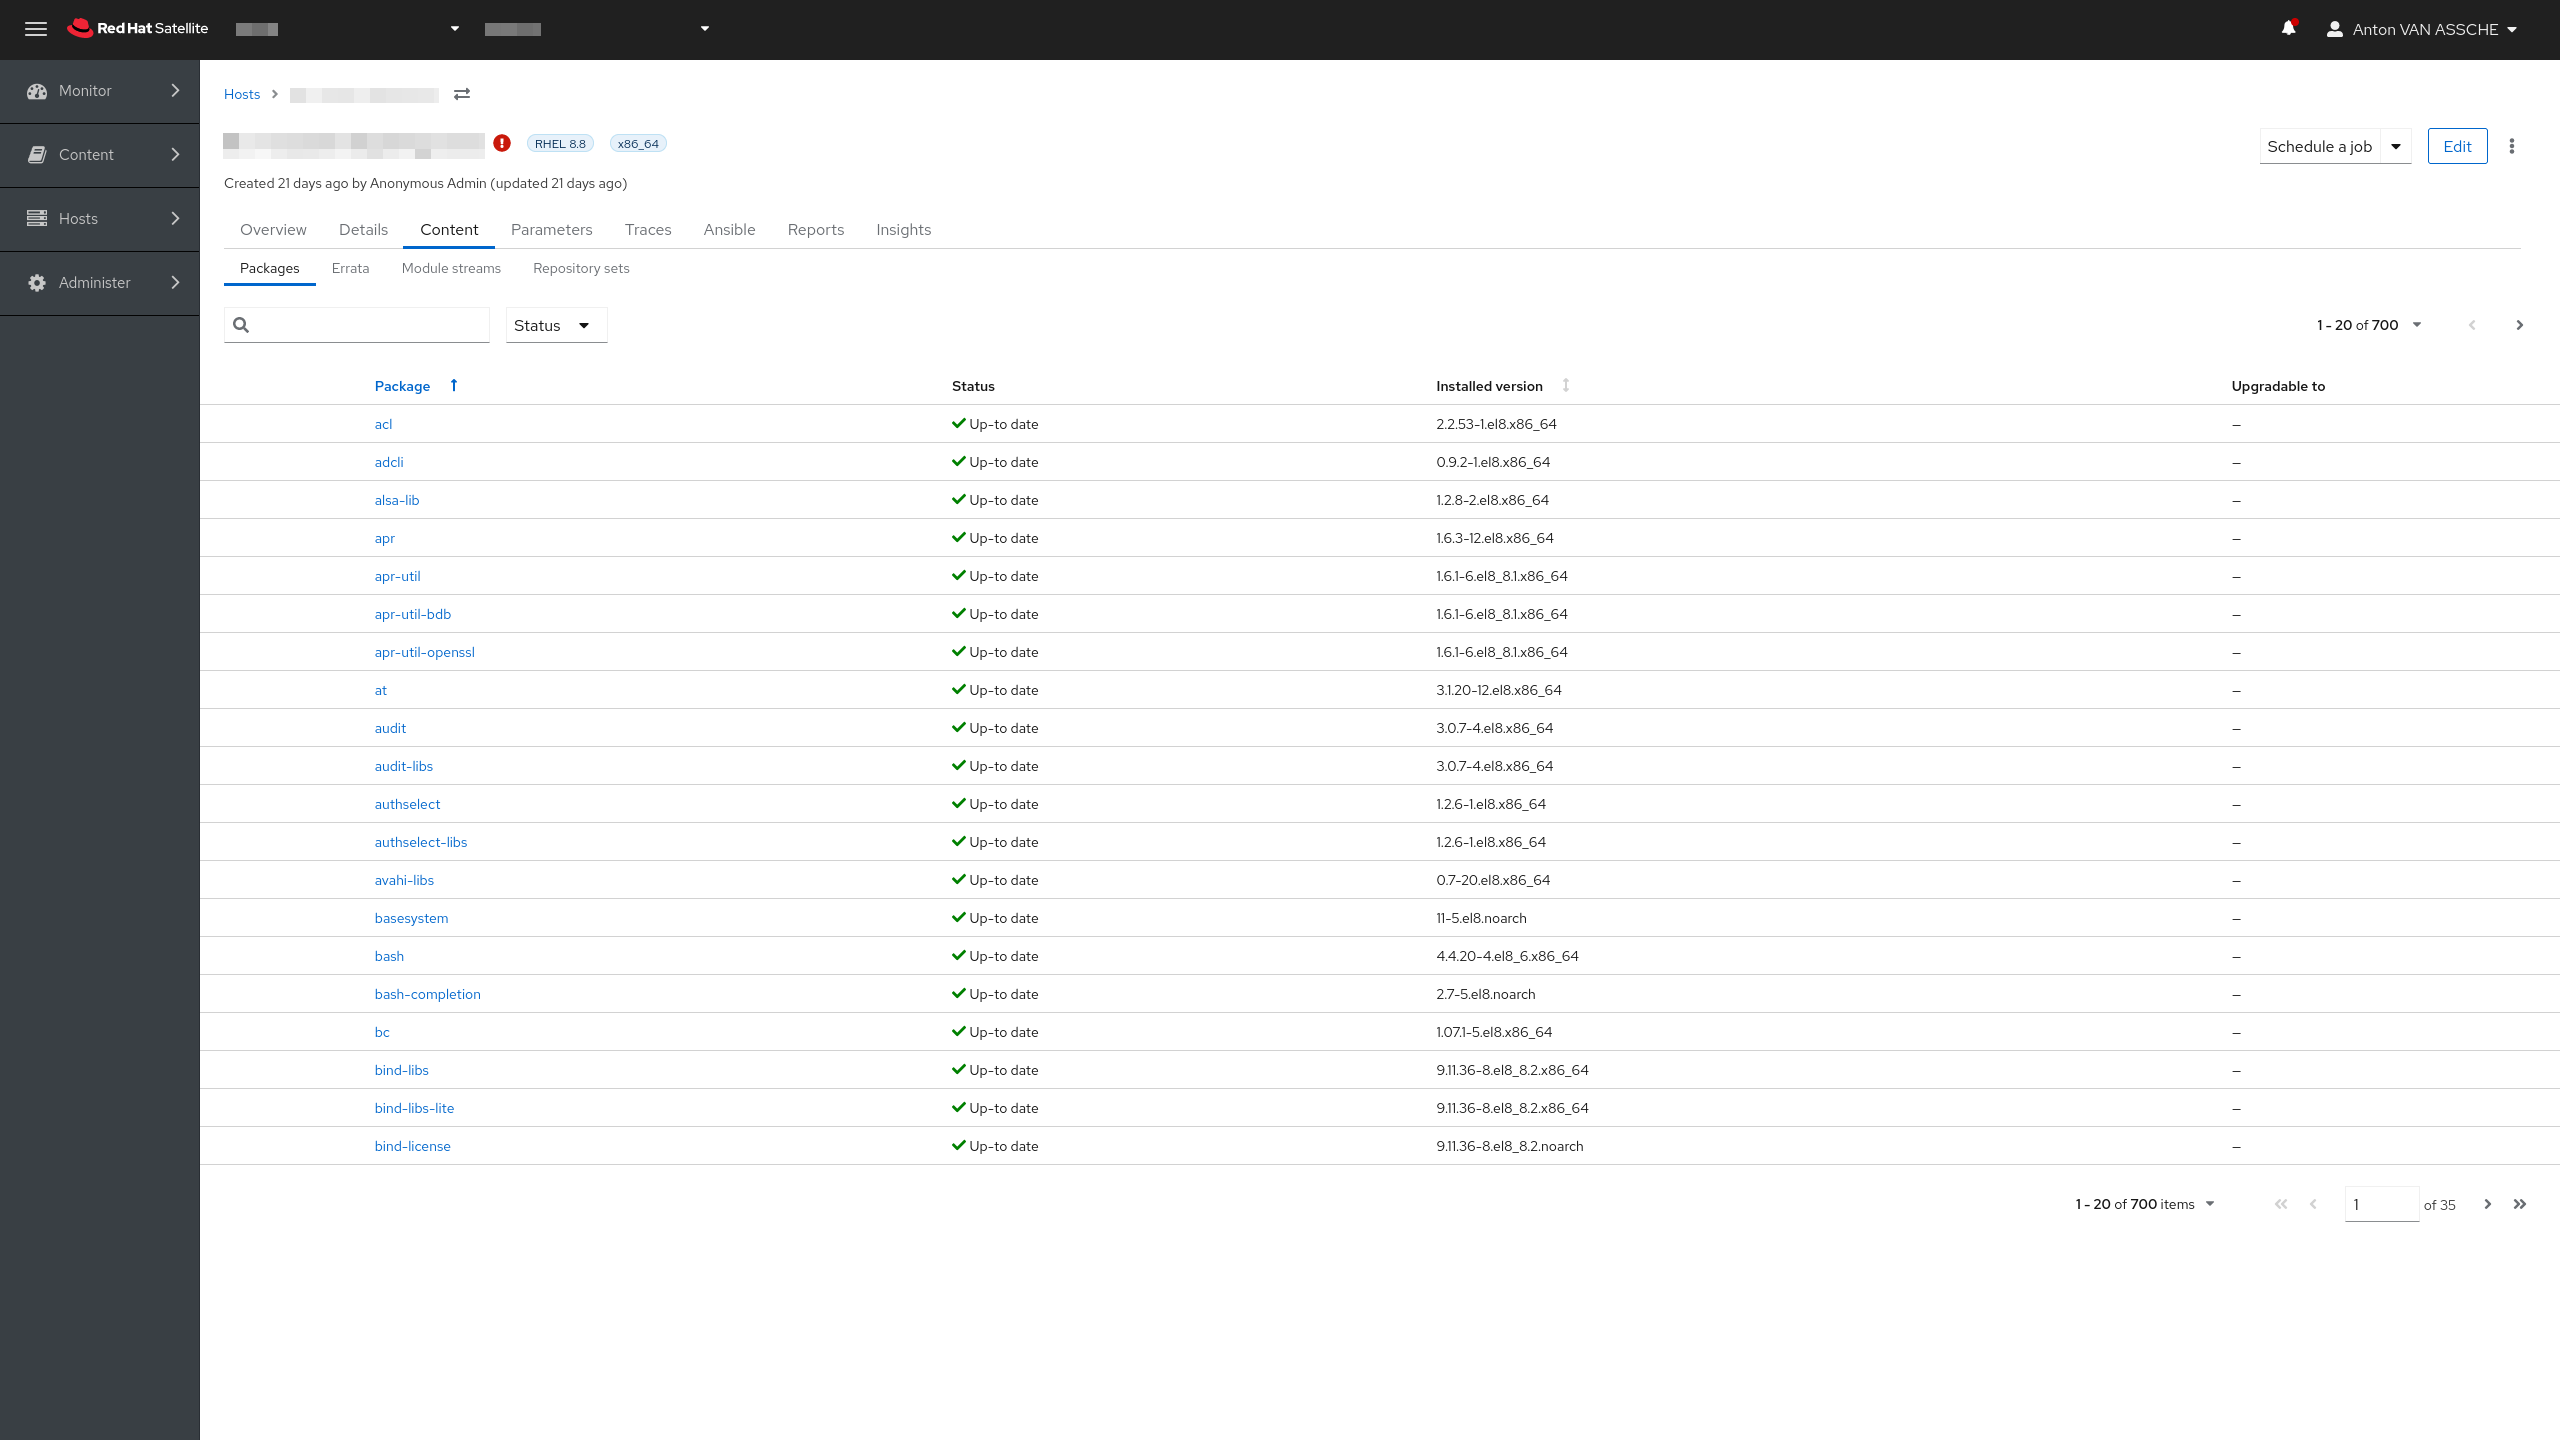
\includegraphics[width=\textwidth]
    {./graphics/state-of-the-art/rhel-satellite/rhel-sat-host-pkgs.png}
    \caption{\label{fig:rhel-sat-host-pkgs}Overzicht van ge\"{i}nstalleerde packages op een host in Red Hat Satellite.}
\end{figure}

%%=============================================================================
%% Nmap
%%=============================================================================

\chapter{\IfLanguageName{dutch}{Uitvoer: ConfiScan}{Output: ConfiScan}}%
\label{ch:bijlage_confiscan}

Deze bijlage presenteert een voorbeeld van de uitvoer van het ontwikkelde script, genaamd ConfiScan.
Het script begint met het identificeren van hardware-informatie, inclusief fabrikant, product, versie en serienummer van de machine.
Daarna wordt informatie over het besturingssysteem verzameld, zoals de kernelversie, kernelmodules en kernelparameters, waaruit kan worden afgeleid dat het een Debian GNU/Linux 12 (bookworm) systeem betreft met kernelversie 6.1.0-18-amd64.

Na het verzamelen van informatie over het besturingssysteem toont het script alle gebruikers en groepen op het systeem, inclusief hun rechten, zoals gebruikersnaam, gebruikers-ID, groeps-ID, shell en home-directory, evenals de \texttt{sudo}-regels ingesteld voor elke gebruiker.

Vervolgens wordt een lijst van alle ge\"installeerde softwarepakketten en hun bronnen (repositories) weergegeven, waarbij een deel van de uitvoer is afgekapt om de leesbaarheid te verbeteren, aangeduid met \texttt{[...]}.

Netwerkgerelateerde gegevens worden ook verzameld, zoals netwerkinterfaces, routingtabel, gebruikte nameservers en firewallregels, inclusief het statische IPv4-adres van \texttt{srv1} (\texttt{172.16.128.1/24}).
Daarnaast worden alle luisterende poorten en hun bijbehorende processen weergegeven, zowel voor TCP als UDP.

Verder wordt informatie verzameld over de schijven op de server en de aanwezige partities, inclusief mountpoints, bestandssystemen en grootte van de partities.

Tot slot worden een lijst van alle systemd-units die zijn ingeschakeld, evenals de opgegeven configuratiebestanden, systemd-units, cronjobs en ssh-configuratie die zijn meegegeven als argumenten voor het script, gekopieerd naar een tarball.

\begin{longlisting}
  \begin{minted}[linenos,tabsize=4,breaklines]{console}
root@srv1:~# ./confiscan.sh -t /etc/bind/named.conf /etc/node_exporter/config.yaml
Info: You are running: ConfiScan v0.8-devel
Info: Using config file(s): /etc/bind/named.conf /etc/node_exporter/config.yaml /etc/ssh/ssh_config /etc/ssh/ssh_config.d/ /etc/ssh/sshd_config /etc/ssh/sshd_config.d/
Info: Creating directories...
Info: Hardware Information:
Info: System Information:
# dmidecode 3.4
Getting SMBIOS data from sysfs.
SMBIOS 2.5 present.

Handle 0x0001, DMI type 1, 27 bytes
System Information
        Manufacturer: innotek GmbH
        Product Name: VirtualBox
        Version: 1.2
        Serial Number: 0
        UUID: 7624a9e2-8b8f-4cf9-8d4d-97a0b5453c05
        Wake-up Type: Power Switch
        SKU Number: Not Specified
        Family: Virtual Machine

Info: Processor Information:
# dmidecode 3.4
Getting SMBIOS data from sysfs.
SMBIOS 2.5 present.

Info: Memory Information:
# dmidecode 3.4
Getting SMBIOS data from sysfs.
SMBIOS 2.5 present.

Info: BIOS Information:
# dmidecode 3.4
Getting SMBIOS data from sysfs.
SMBIOS 2.5 present.

Handle 0x0000, DMI type 0, 20 bytes
BIOS Information
        Vendor: innotek GmbH
        Version: VirtualBox
        Release Date: 12/01/2006
        Address: 0xE0000
        Runtime Size: 128 kB
        ROM Size: 128 kB
        Characteristics:
                ISA is supported
                PCI is supported
                Boot from CD is supported
                Selectable boot is supported
                8042 keyboard services are supported (int 9h)
                CGA/mono video services are supported (int 10h)
                ACPI is supported

Info: OS Information:
Hostname  OperatingSystem  Name                            Version  Version_ID     Codename  Kernel
srv1      GNU/Linux        Debian GNU/Linux 12 (bookworm)  12       12 (bookworm)  bookworm  6.1.0-18-amd64
Info: Boot parameters:
BOOT_IMAGE=/boot/vmlinuz-6.1.0-18-amd64
root=UUID=e40706ce-053f-451f-b6fe-0979430677a4
ro
consoleblank=0
elevator=noop
scsi_mod.use_blk_mq=Y
net.ifnames=0
biosdevname=0
BOOT_IMAGE=/boot/vmlinuz-6.1.0-18-amd64
root=UUID=e40706ce-053f-451f-b6fe-0979430677a4
ro
consoleblank=0
elevator=noop
scsi_mod.use_blk_mq=Y
net.ifnames=0
biosdevname=0
Info: Kernel modules:
Module               Size    UsedBy
vboxsf               45056   1 -
intel_rapl_msr       20480   0 -
intel_rapl_common    32768   1 intel_rapl_msr
intel_pmc_core       53248   0 -
ghash_clmulni_intel  16384   0 -
sha512_ssse3         49152   0 -
sha512_generic       16384   1 sha512_ssse3
sha256_ssse3         32768   0 -
sha1_ssse3           32768   0 -
binfmt_misc          24576   1 -
aesni_intel          393216  0 -
crypto_simd          16384   1 aesni_intel
vmwgfx               376832  1 -
cryptd               28672   2 ghash_clmulni_intel crypto_simd
rapl                 20480   0 -
drm_ttm_helper       16384   1 vmwgfx
joydev               28672   0 -
ttm                  94208   2 vmwgfx drm_ttm_helper
drm_kms_helper       204800  1 vmwgfx
vboxguest            49152   1 vboxsf
ac                   20480   0 -
button               24576   0 -
evdev                28672   3 -
serio_raw            20480   0 -
sg                   40960   0 -
drm                  614400  5 vmwgfx drm_ttm_helper ttm drm_kms_helper
fuse                 176128  1 -
loop                 32768   0 -
efi_pstore           16384   0 -
configfs             57344   1 -
dm_mod               184320  0 -
ip_tables            36864   0 -
x_tables             61440   1 ip_tables
autofs4              53248   2 -
ext4                 983040  1 -
crc16                16384   1 ext4
mbcache              16384   1 ext4
jbd2                 167936  1 ext4
crc32c_generic       16384   0 -
sd_mod               65536   1 -
t10_pi               16384   1 sd_mod
crc64_rocksoft       20480   1 t10_pi
crc64                20480   1 crc64_rocksoft
crc_t10dif           20480   1 t10_pi
crct10dif_generic    16384   0 -
ahci                 49152   1 -
libahci              49152   1 ahci
libata               401408  2 ahci libahci
crct10dif_pclmul     16384   1 -
crct10dif_common     16384   3 crc_t10dif crct10dif_generic crct10dif_pclmul
crc32_pclmul         16384   0 -
scsi_mod             286720  3 sg sd_mod libata
psmouse              184320  0 -
crc32c_intel         24576   2 -
i2c_piix4            28672   0 -
scsi_common          16384   3 sg libata scsi_mod
e1000                163840  0 -
floppy               86016   0 -
video                65536   0 -
battery              28672   0 -
wmi                  36864   1 video
Info: Users found on the system:
Username          UID    GID    Shell              Home
root              0      0      /bin/bash          /root
daemon            1      1      /usr/sbin/nologin  /usr/sbin
bin               2      2      /usr/sbin/nologin  /bin
sys               3      3      /usr/sbin/nologin  /dev
sync              4      65534  /bin/sync          /bin
games             5      60     /usr/sbin/nologin  /usr/games
man               6      12     /usr/sbin/nologin  /var/cache/man
lp                7      7      /usr/sbin/nologin  /var/spool/lpd
mail              8      8      /usr/sbin/nologin  /var/mail
news              9      9      /usr/sbin/nologin  /var/spool/news
uucp              10     10     /usr/sbin/nologin  /var/spool/uucp
proxy             13     13     /usr/sbin/nologin  /bin
www-data          33     33     /usr/sbin/nologin  /var/www
backup            34     34     /usr/sbin/nologin  /var/backups
list              38     38     /usr/sbin/nologin  /var/list
irc               39     39     /usr/sbin/nologin  /run/ircd
_apt              42     65534  /usr/sbin/nologin  /nonexistent
messagebus        100    106    /usr/sbin/nologin  /nonexistent
_chrony           101    109    /usr/sbin/nologin  /var/lib/chrony
sshd              102    65534  /usr/sbin/nologin  /run/sshd
bind              103    110    /usr/sbin/nologin  /var/cache/bind
systemd-timesync  997    997    /usr/sbin/nologin  /
systemd-network   998    998    /usr/sbin/nologin  /
node-exp          999    100    /usr/sbin/nologin  /
vagrant           1000   1000   /bin/bash          /home/vagrant
nobody            65534  65534  /usr/sbin/nologin  /nonexistent
Info: Privileged users:

Info: Custom sudo rules for each user:
Username  Privilege
root      (ALL : ALL) ALL
vagrant   (ALL) NOPASSWD: ALL
Info: Groups found on the system:
Groupname         GID    Members
root              0
daemon            1
bin               2
sys               3
adm               4
tty               5
disk              6
lp                7
mail              8
news              9
uucp              10
man               12
proxy             13
kmem              15
dialout           20
fax               21
voice             22
cdrom             24
floppy            25
tape              26
sudo              27
audio             29
dip               30
www-data          33
backup            34
operator          37
list              38
irc               39
src               40
shadow            42
utmp              43
video             44
sasl              45
plugdev           46
staff             50
games             60
users             100
nogroup           65534
crontab           101
systemd-journal   999
systemd-network   998
systemd-timesync  997
input             102
sgx               103
kvm               104
render            105
messagebus        106
_ssh              107
netdev            108
_chrony           109
vagrant           1000
bind              110
node-exp          996    node-exp
Info: Package info:
Info: Packages found on the system:
Package                     Version                         Architecture
adduser                     3.134                           all
apparmor                    3.0.8-3                         amd64
apt                         2.6.1                           amd64
apt-listchanges             3.24                            all
apt-utils                   2.6.1                           amd64         apt
base-files                  12.4+deb12u5                    amd64
base-passwd                 3.6.1                           amd64
bash                        5.2.15-2+b2                     amd64         bash (5.2.15-2)
bash-completion             1:2.11-6                        all
bind9                       1:9.18.24-1                     amd64
bind9-dnsutils              1:9.18.24-1                     amd64         bind9
bind9-host                  1:9.18.24-1                     amd64         bind9
bind9-libs                  1:9.18.24-1                     amd64         bind9
bind9-utils                 1:9.18.24-1                     amd64         bind9
bind9utils                  1:9.18.24-1                     all           bind9
[...]
Info: Package repositories:
deb https://deb.debian.org/debian bookworm main
deb-src https://deb.debian.org/debian bookworm main
deb https://security.debian.org/debian-security bookworm-security main
deb-src https://security.debian.org/debian-security bookworm-security main
deb https://deb.debian.org/debian bookworm-updates main
deb-src https://deb.debian.org/debian bookworm-updates main
deb https://deb.debian.org/debian bookworm-backports main
deb-src https://deb.debian.org/debian bookworm-backports main
Info: Network devices:
Device  IPv4          Netmask        Broadcast       IPv6                      Prefix  DHCP   DHCPServer
lo      127.0.0.1     255.0.0.0      N/A             ::1                       128     false  N/A
eth0    10.0.2.15     255.255.255.0  10.0.2.255      fe80::a00:27ff:fe8d:c04d  64      true   10.0.2.2
eth1    172.16.128.1  255.255.0.0    172.16.255.255  fe80::a00:27ff:feec:112e  64      false  N/A
Info: Routing table:
Destination  Gateway   Genmask        Flags  Metric  Ref  Use  Iface
0.0.0.0      10.0.2.2  0.0.0.0        UG     0       0    0    eth0
10.0.2.0     0.0.0.0   255.255.255.0  U      0       0    0    eth0
172.16.0.0   0.0.0.0   255.255.0.0    U      0       0    0    eth1
Info: Nameservers:
Nameserver
172.16.128.1
Info: Firewall rules:
Chain INPUT (policy ACCEPT 0 packets, 0 bytes)
 pkts bytes target     prot opt in     out     source               destination

Chain FORWARD (policy ACCEPT 0 packets, 0 bytes)
 pkts bytes target     prot opt in     out     source               destination

Chain OUTPUT (policy ACCEPT 0 packets, 0 bytes)
 pkts bytes target     prot opt in     out     source               destination
Info: Listening ports (TCP):
State   Recv-Q  Send-Q  Local                               Address:Port  Peer                     Address:PortProcess
LISTEN  0       5       127.0.0.1:953                       0.0.0.0:*     users:(("named"          pid=11774            fd=24))
LISTEN  0       5       127.0.0.1:953                       0.0.0.0:*     users:(("named"          pid=11774            fd=51))
LISTEN  0       128     0.0.0.0:22                          0.0.0.0:*     users:(("sshd"           pid=603              fd=3))
LISTEN  0       10      10.0.2.15:53                        0.0.0.0:*     users:(("named"          pid=11774            fd=33))
LISTEN  0       10      10.0.2.15:53                        0.0.0.0:*     users:(("named"          pid=11774            fd=34))
LISTEN  0       10      127.0.0.1:53                        0.0.0.0:*     users:(("named"          pid=11774            fd=27))
LISTEN  0       10      127.0.0.1:53                        0.0.0.0:*     users:(("named"          pid=11774            fd=28))
LISTEN  0       5       127.0.0.1:8053                      0.0.0.0:*     users:(("named"          pid=11774            fd=55))
LISTEN  0       5       127.0.0.1:8053                      0.0.0.0:*     users:(("named"          pid=11774            fd=56))
LISTEN  0       10      172.16.128.1:53                     0.0.0.0:*     users:(("named"          pid=11774            fd=37))
LISTEN  0       10      172.16.128.1:53                     0.0.0.0:*     users:(("named"          pid=11774            fd=38))
LISTEN  0       10      [fe80::a00:27ff:feec:112e]%eth1:53  [::]:*        users:(("named"          pid=11774            fd=50))
LISTEN  0       10      [fe80::a00:27ff:feec:112e]%eth1:53  [::]:*        users:(("named"          pid=11774            fd=49))
LISTEN  0       128     [::]:22                             [::]:*        users:(("sshd"           pid=603              fd=4))
LISTEN  0       10      [::1]:53                            [::]:*        users:(("named"          pid=11774            fd=41))
LISTEN  0       10      [::1]:53                            [::]:*        users:(("named"          pid=11774            fd=42))
LISTEN  0       4096    *:9100                              *:*           users:(("node_exporter"  pid=12680            fd=3))
LISTEN  0       5       [::1]:953                           [::]:*        users:(("named"          pid=11774            fd=53))
LISTEN  0       5       [::1]:953                           [::]:*        users:(("named"          pid=11774            fd=52))
LISTEN  0       10      [fe80::a00:27ff:fe8d:c04d]%eth0:53  [::]:*        users:(("named"          pid=11774            fd=46))
LISTEN  0       10      [fe80::a00:27ff:fe8d:c04d]%eth0:53  [::]:*        users:(("named"          pid=11774            fd=45))
Info: Listening ports (UDP):
State   Recv-Q  Send-Q  Local                               Address:Port  Peer                Address:PortProcess
UNCONN  0       0       172.16.128.1:53                     0.0.0.0:*     users:(("named"     pid=11774            fd=35))
UNCONN  0       0       172.16.128.1:53                     0.0.0.0:*     users:(("named"     pid=11774            fd=36))
UNCONN  0       0       10.0.2.15:53                        0.0.0.0:*     users:(("named"     pid=11774            fd=31))
UNCONN  0       0       10.0.2.15:53                        0.0.0.0:*     users:(("named"     pid=11774            fd=32))
UNCONN  0       0       127.0.0.1:53                        0.0.0.0:*     users:(("named"     pid=11774            fd=25))
UNCONN  0       0       127.0.0.1:53                        0.0.0.0:*     users:(("named"     pid=11774            fd=26))
UNCONN  0       0       127.0.0.1:323                       0.0.0.0:*     users:(("chronyd"   pid=417              fd=5))
UNCONN  0       0       0.0.0.0:68                          0.0.0.0:*     users:(("dhclient"  pid=1188             fd=7))
UNCONN  0       0       [::1]:53                            [::]:*        users:(("named"     pid=11774            fd=40))
UNCONN  0       0       [::1]:53                            [::]:*        users:(("named"     pid=11774            fd=39))
UNCONN  0       0       [fe80::a00:27ff:fe8d:c04d]%eth0:53  [::]:*        users:(("named"     pid=11774            fd=44))
UNCONN  0       0       [fe80::a00:27ff:fe8d:c04d]%eth0:53  [::]:*        users:(("named"     pid=11774            fd=43))
UNCONN  0       0       [fe80::a00:27ff:feec:112e]%eth1:53  [::]:*        users:(("named"     pid=11774            fd=48))
UNCONN  0       0       [fe80::a00:27ff:feec:112e]%eth1:53  [::]:*        users:(("named"     pid=11774            fd=47))
UNCONN  0       0       [::1]:323                           [::]:*        users:(("chronyd"   pid=417              fd=6))
Info: Disk info:
Disk      Size  Bytes        Sectors
/dev/sda  20    21474836480  41943040
Info: Partitions:
Device     Boot  Start  End       Sectors   Size  ID  Type
/dev/sda1  *     2048   41943039  41940992  20G   83  Linux
Info: Used filesystems:
Filesystem   IsUsed
sysfs        false
tmpfs        false
bdev         false
proc         false
cgroup       false
cgroup2      false
cpuset       false
devtmpfs     false
debugfs      false
tracefs      false
securityfs   false
sockfs       false
bpf          false
pipefs       false
ramfs        false
hugetlbfs    false
devpts       false
mqueue       false
pstore       false
ext3         true
ext2         true
ext4         true
autofs       false
configfs     false
fuseblk      true
fuse         false
fusectl      false
binfmt_misc  false
vboxsf       false
Info: Mount points:
Device       MountPoint                                           FSType       Options
sysfs        /sys                                                 sysfs        rw nosuid nodev noexec relatime                                                          0  0
proc         /proc                                                proc         rw nosuid nodev noexec relatime                                                          0  0
udev         /dev                                                 devtmpfs     rw nosuid relatime size=211652k nr_inodes=52913 mode=755 inode64                         0  0
devpts       /dev/pts                                             devpts       rw nosuid noexec relatime gid=5 mode=620 ptmxmode=000                                    0  0
tmpfs        /run                                                 tmpfs        rw nosuid nodev noexec relatime size=46828k mode=755 inode64                             0  0
/dev/sda1    /                                                    ext4         rw relatime discard errors=remount-ro                                                    0  0
securityfs   /sys/kernel/security                                 securityfs   rw nosuid nodev noexec relatime                                                          0  0
tmpfs        /dev/shm                                             tmpfs        rw nosuid nodev inode64                                                                  0  0
tmpfs        /run/lock                                            tmpfs        rw nosuid nodev noexec relatime size=5120k inode64                                       0  0
cgroup2      /sys/fs/cgroup                                       cgroup2      rw nosuid nodev noexec relatime nsdelegate memory_recursiveprot                          0  0
pstore       /sys/fs/pstore                                       pstore       rw nosuid nodev noexec relatime                                                          0  0
bpf          /sys/fs/bpf                                          bpf          rw nosuid nodev noexec relatime mode=700                                                 0  0
systemd-1    /proc/sys/fs/binfmt_misc                             autofs       rw relatime fd=30 pgrp=1 timeout=0 minproto=5 maxproto=5 direct pipe_ino=13461           0  0
hugetlbfs    /dev/hugepages                                       hugetlbfs    rw relatime pagesize=2M                                                                  0  0
mqueue       /dev/mqueue                                          mqueue       rw nosuid nodev noexec relatime                                                          0  0
debugfs      /sys/kernel/debug                                    debugfs      rw nosuid nodev noexec relatime                                                          0  0
tracefs      /sys/kernel/tracing                                  tracefs      rw nosuid nodev noexec relatime                                                          0  0
configfs     /sys/kernel/config                                   configfs     rw nosuid nodev noexec relatime                                                          0  0
fusectl      /sys/fs/fuse/connections                             fusectl      rw nosuid nodev noexec relatime                                                          0  0
ramfs        /run/credentials/systemd-sysctl.service              ramfs        ro nosuid nodev noexec relatime mode=700                                                 0  0
ramfs        /run/credentials/systemd-sysusers.service            ramfs        ro nosuid nodev noexec relatime mode=700                                                 0  0
ramfs        /run/credentials/systemd-tmpfiles-setup-dev.service  ramfs        ro nosuid nodev noexec relatime mode=700                                                 0  0
ramfs        /run/credentials/systemd-tmpfiles-setup.service      ramfs        ro nosuid nodev noexec relatime mode=700                                                 0  0
binfmt_misc  /proc/sys/fs/binfmt_misc                             binfmt_misc  rw nosuid nodev noexec relatime                                                          0  0
tmpfs        /run/user/1000                                       tmpfs        rw nosuid nodev relatime size=46828k nr_inodes=11707 mode=700 uid=1000 gid=1000 inode64  0  0
vagrant      /vagrant                                             vboxsf       rw relatime                                                                              0  0
Info: Enabled systemd units:
Unit                         State    Preset
apparmor.service             enabled  enabled
chrony.service               enabled  enabled
cron.service                 enabled  enabled
e2scrub_reap.service         enabled  enabled
getty@.service               enabled  enabled
named.service                enabled  enabled
networking.service           enabled  enabled
node_exporter.service        enabled  enabled
rsyslog.service              enabled  enabled
ssh.service                  enabled  enabled
systemd-pstore.service       enabled  enabled
unattended-upgrades.service  enabled  enabled
remote-fs.target             enabled  enabled
apt-daily-upgrade.timer      enabled  enabled
apt-daily.timer              enabled  enabled
dpkg-db-backup.timer         enabled  enabled
e2scrub_all.timer            enabled  enabled
fstrim.timer                 enabled  enabled
logrotate.timer              enabled  enabled
man-db.timer                 enabled  enabled
Info: Getting: /etc/bind/named.conf
Info: Getting: /etc/node_exporter/config.yaml
Info: Getting: /etc/ssh/ssh_config
Info: Getting: /etc/ssh/ssh_config.d/
Info: Getting: /etc/ssh/sshd_config
Info: Getting: /etc/ssh/sshd_config.d/
Info: Getting: /etc/systemd/system/
Info: Getting: /etc/systemd/user/
Info: Getting: /usr/lib/systemd/system/
Info: Getting: /etc/cron.d
Info: Getting: /etc/cron.daily
Info: Getting: /etc/cron.weekly
Info: Getting: /etc/cron.monthly
Info: Creating tarball...
  \end{minted}
  \caption[Uitvoer van ConfiScan op \texttt{srv1}.]{De uitvoer van het ConfiScan script op srv1.}
  \label{lst:bijlage-confiscan}
\end{longlisting}

%%=============================================================================
%% PoC uitvoering
%%=============================================================================

\chapter{\IfLanguageName{dutch}{Uitvoer: Proof of Concept}{Execution: Proof of Concept}}
\label{ch:bijlage_poc_uitvoering}

Deze bijlage biedt een uitgebreide beschrijving van de uitvoering van de Proof of Concept op de vijf servers.

Om het script op een reproduceerbare manier uit te voeren, is gebruik gemaakt van een Ansible playbook.
Het script heeft enkele vereisten, namelijk: \texttt{net-tools} en \texttt{dmidecode}, zoals te zien in listing~\ref{lst:bijlage-requirements}.
Het \texttt{net-tools} pakket wordt gebruikt om de configuratie van de netwerkinterfaces te verzamelen, terwijl \texttt{dmidecode} wordt gebruikt om de hardware-informatie van de servers te verzamelen.

\begin{listing}
  \begin{minted}[linenos,tabsize=4,breaklines]{yaml}
- name: Install required packages
  ansible.builtin.apt:
    name:
      - net-tools
      - dmidecode
    state: latest
    update_cache: yes
  \end{minted}
  \caption[Installatie van vereiste pakketten.]{Code verantwoordelijk voor het installeren van de vereiste pakketten}
  \label{lst:bijlage-requirements}
\end{listing}

\begin{listing}
  \begin{minted}[linenos,tabsize=4,breaklines]{yaml}
- name: Install ConfiScan
  ansible.builtin.copy:
    src: /vagrant/ansible/files/confiscan.sh
    dest: /tmp/confiscan.sh
  \end{minted}
  \caption[Kopi\"{e}ren van script naar servers.]{Code verantwoordelijk voor het kopiëren van het script naar de servers}
  \label{lst:bijlage-copy-script}
\end{listing}

Het Ansible playbook plaatst eerst het script, dat vooraf moet worden geplaatst in \texttt{src/poc/ansible/files/}, op de servers in de map \texttt{/tmp/}, zoals te zien in listing \ref{lst:bijlage-copy-script}.
Daar wordt het script vervolgens uitgevoerd met de \texttt{-t} optie, gevolgd door de paden van de configuraties die men wil opnemen in ons inventaris.
Zoals weergegeven in listing \ref{lst:bijlage-run-script}, wordt het script uitgevoerd op \texttt{srv1}.
Nadat het script op elke server is uitgevoerd, downloadt en plaatst het playbook de tarballs van elke server in de home directory van de gebruiker die het playbook uitvoert.
Ten slotte worden de tarballs uitgepakt aan het einde van het playbook.
De laatste twee stappen zijn te zien in listing \ref{lst:bijlage-tarballs}.
Listing~\ref{lst:bijlage-run-playbook} illustreert hoe men aan de hand van het playbook het script kunnen uitvoeren op elke server.
Om de uitvoer de playbook te bekijken, zie de GitHub-repository van de Proof of Concept~\autocite{github-poc}.

\begin{listing}
  \begin{minted}[linenos,tabsize=4,breaklines]{yaml}
- name: ConfiScan on srv1
  hosts:
    - srv1
  gather_facts: no
  tasks:
    - name: Runs script
      ansible.builtin.shell: /tmp/confiscan.sh -t /etc/bind/named.conf /etc/node_exporter/config.yaml
      args:
        chdir: /tmp/
      become: true
    \end{minted}
    \caption[Uitvoeren van script op \texttt{srv1}.]{Code verantwoordelijk voor het uitvoeren van het script op srv1}
    \label{lst:bijlage-run-script}
\end{listing}

\begin{listing}
  \begin{minted}[linenos,tabsize=4,breaklines]{yaml}
- name: Download tarballs
  hosts:
    - servers
  gather_facts: no
  tasks:
    - name: Copy tarballs
      ansible.builtin.fetch:
        src: "/tmp/{{ inventory_hostname }}-configs.tar.gz"
        dest: "{{ lookup('ansible.builtin.env', 'HOME') }}"
        owner: "{{ lookup('ansible.builtin.env', 'USER') }}"
        group: "{{ lookup('ansible.builtin.env', 'USER') }}"
    - name: Extracting tarballs
      ansible.builtin.unarchive:
        src: "{{ lookup('ansible.builtin.env', 'HOME') }}/{{ inventory_hostname }}/tmp/{{ inventory_hostname }}-configs.tar.gz"
        dest: "{{ lookup('ansible.builtin.env', 'HOME') }}/"
      delegate_to: localhost
  \end{minted}
  \caption[Downloaden en uitpakken van tarballs.]{Code verantwoordelijk voor het downloaden en uitpakken van de tarballs}
  \label{lst:bijlage-tarballs}
\end{listing}

\begin{listing}
  \begin{minted}[linenos,tabsize=4,breaklines]{console}
[vagrant@control ~]$ cd /vagrant/ansible/
[vagrant@control ~]$ ansible-playbook -i inventory.yml poc.yml
  \end{minted}
  \caption[Uitvoeren van Ansible playbook.]{Instructies voor het uitvoeren van de Ansible playbook die het script uitvoert op elke server.}
  \label{lst:bijlage-run-playbook}
\end{listing}

Echter kan men ook het script handmatig uitvoeren op elke server.
Hiervoor moet men eerst inloggen op de server en het script vanuit \texttt{/vagrant/ansible/files/} kopi\"eren naar een gewenste locatie.
In \ref{lst:bijlage-run-script-manual} wordt gedemonstreerd hoe dit handmatig kan worden gedaan op \texttt{srv1}.

Men gebruikt de \texttt{-t} optie om aan te geven dat men aan het einde een tarball wil verkrijgen in plaats van een directory genaamd \texttt{srv1-configs}.
Daarna specificeert men de gewenste configuratiebestanden die men wil opnemen in de inventaris.

Merk op dat het script moet worden uitgevoerd met root-privileges.
Dit kan worden bereikt door in te loggen als de root-gebruiker of door het gebruik van het \texttt{sudo}-commando.

\begin{listing}
  \begin{minted}[linenos,tabsize=4,breaklines]{console}
root@srv1:~# cp /vagrant/ansible/files/confiscan.sh ~
root@srv1:~# ./confiscan.sh -t \
    /etc/bind/named.conf \
    /etc/node_exporter/config.yaml
  \end{minted}
  \caption[Manueel uitvoeren van script op \texttt{srv1}.]{Instructies om het script manueel uit te voeren op \texttt{srv1}.}
  \label{lst:bijlage-run-script-manual}
\end{listing}

%%=============================================================================
%% Symlink kopïeren met rsync
%%=============================================================================

\chapter{\IfLanguageName{dutch}{Oplossing: Symlinks kopi\"{e}ren met rsync}{Solution: Copying symlinks with rsync}}
\label{ch:bijlage_symlink_kopieren_met_rsync}

Deze bijlage presenteert een alternatieve oplossing voor het kopi\"eren van symlinks, een beperking van de huidige implementatie van het script.
In de diff van~\ref{lst:bijlage-rsync-copy-alternative-diff} is te zien dat we \texttt{cp} vervangen door \texttt{rsync}, gevolgd door enkele opties die ervoor zorgen dat de symlink wordt gevolgd en het effectieve bestand wordt gekopieerd.
Een korte uitleg van de gebruikte opties:

\begin{itemize}
  \item \texttt{--force}: Overschrijf bestaande bestanden.
  \item \texttt{--archive}: Archiveer bestanden en directories recursief.
  \item \texttt{--recursive}: Kopieer directories recursief.
  \item \texttt{--copy-links}: Kopieer symlinks als een bestand en volg de link naar het effectieve bestand.
\end{itemize}

Echter, deze operatie zal falen op Debian-systemen, omdat enkele symlinks in\\ \texttt{/etc/systemd/system/} verwijzen naar bestanden die niet bestaan.
Om dit probleem op te lossen, is \texttt{|| :} toegevoegd aan het einde van het commando.
Dit zorgt ervoor dat de operatie nooit faalt, zelfs als er een fout optreedt.

Echter betekent dit ook dat andere fouten niet correct zullen worden afgehandeld, wat de robuustheid van het script kan verminderen.
Dit is dan ook de redenen waarom deze oplossing niet werd ge\"implementeerd in de uiteindelijke versie van het script.

Uiteindelijk moeten we ook de playbook aanpassen zodat het script op elk systeem wordt uitgevoerd.
De benodigde aanpassing omvat het toevoegen van \texttt{rsync} aan de lijst van vereiste pakketten, zoals weergegeven in~\ref{lst:bijlage-rsync-playbook-diff}.

\begin{listing}
  \begin{minted}[linenos,tabsize=4,breaklines]{diff}
diff --git a/src/tool/confiscan.sh b/src/tool/confiscan.sh
index 231954e..0e5acc8 100755
--- a/src/tool/confiscan.sh
+++ b/src/tool/confiscan.sh
@@ -427,7 +427,7 @@ for c in "${APP_CONFIGS[@]}"; do
         error "${c} no such file or directory." 2

     mkdir -p "${output_dir}/$(dirname "${c}")"
-    cp -r "${c}" "${output_dir}/$(dirname "${c}")"
+    rsync --force --archive --recursive --copy-links "${c}" "${output_dir}/$(dirname "${c}")" || :
 done

 # File Integrity Check of original files, excluding ./original.sha256
  \end{minted}
  \caption{Alternatieve aanpak om symlinks ook te kopi\"{e}ren.}
  \label{lst:bijlage-rsync-copy-alternative-diff}
\end{listing}

\begin{listing}
  \begin{minted}[linenos,tabsize=4,breaklines]{diff}
diff --git a/src/poc/ansible/poc.yml b/src/poc/ansible/poc.yml
index 1010ed1..24ffd3e 100644
--- a/src/poc/ansible/poc.yml
+++ b/src/poc/ansible/poc.yml
@@ -8,6 +8,7 @@
         name:
           - net-tools
           - dmidecode
+          - rsync
         state: latest
  \end{minted}
  \caption{Aanpassing van de playbook om \texttt{rsync} te installeren.}
  \label{lst:bijlage-rsync-playbook-diff}
\end{listing}


%%---------- Andere bijlagen --------------------------------------------------

%%---------- Backmatter, referentielijst ---------------------------------------

\backmatter{}

\setlength\bibitemsep{2pt} %% Add Some space between the bibliograpy entries
\printbibliography[heading=bibintoc]

\end{document}
